% this package is designed by: thanhhungqb@gmail.com
% more information and update: 
%   https://github.com/thanhhungqb/thesis-template
\documentclass[12pt,a4paper,oneside]{book} % twoside for draft

%\usepackage{babel}
%\usepackage[utf8]{vietnam}
%\usepackage{times}
%\usepackage{graphicx}
\usepackage{amssymb}

%\usepackage{mathptmx}	% same Time New Roma
%\renewcommand{\rmdefault}{phv} % Arial
%\renewcommand{\sfdefault}{phv} % Arial

\usepackage{fancyhdr}
\usepackage{algorithm2e}
\usepackage{mathtools}
\usepackage{makecell}
\usepackage{tikz}
\usetikzlibrary{matrix}
\usepackage{nicematrix}
\usepackage{siunitx}
\usepackage{karnaugh-map}
\usepackage{bkthesis}

\addbibresource{refs.bib}

%\csdeptname{KHOA ĐIỆN ĐIỆN TỬ}
%\crname{BÁO CÁO THỰC TẬP TỐT NGHIỆP}
% \crname{BÁO CÁO TIỂU LUẬN}
\title{EE4423: COMPUTER ARCHITECTURE}
\subtitle{Milestone 2: A Single-Cycle Processor}
\csSupervise{Dr. Trần Hoàng Linh}
\csSubject{Computer Architecture}
    \cttime{November 11, 2023}

\thesislayout

\begin{document}
%-	Bìa cứng - màu xanh dương, chữ mạ vàng (xem mẫu đính kèm)
%-	Trang tên (tờ lót): chất liệu giấy, nội dung giống như bìa LV
%-	Ở gáy LV: in nhan đề LV (có thể in tóm tắt nếu nhan đề quá dài), size 15 – 17
%-	Phiếu Nhiệm vụ LV, chấm điểm Hướng dẫn & Phản biện (đã ký): nhận từ GVHD & GVPB sau khi bảo vệ (theo lịch hẹn).
%-	Lời cam đoan
%-	Lời cảm ơn/ Lời ngỏ
%-	Tóm tắt LV
%-	Mục lục
%-	Danh mục, bảng biểu, hình ảnh, ... (nếu có)
%-	Nội dung LV
%-	Danh mục TL tham khảo
%-	Phụ lục (nếu có)

\coverpage

\frontmatter

%\newpage
\pagestyle{fancy}
%\pagestyle{fancy}  % Finally, use the "fancy" page style to implement the FancyHdr headers
%\fancyhead{}  % Clears all page headers and footers
%\rhead{Instructor: \begin{otherlanguage}{vietnamese}Dr. Trần Hoàng Linh\end{otherlanguage}}  % Sets the right side header to show the page number
%\lhead{\subtitle}  % Clears the left side page header

\tableofcontents
%%\listofsymbols
%\newpage
\listoffigures
%\newpage
%\listoftables
%%\listofalgorithms
%\newpage
%\lstlistoflistings


\mainmatter

% \chapter{Objectives}
% \section{Review understanding of basic logic design}
% Basic logic design encompasses the fundamental principles and techniques used to design and implement digital circuits. At its core are logic gates, which are electronic components that perform logical operations on binary signals. These gates, including AND, OR, NOT, NAND, NOR, and XOR gates, form the building blocks of digital systems. By combining these gates in different configurations, complex logical functions and operations can be realized.

% Understanding basic logic design principles is essential for designing various digital systems, such as processors, memory units, and control units. It provides the foundation for implementing logical operations, processing binary data, and realizing complex functionalities in digital electronics.

% \section{Review understanding of basic logic FSM}
% A Finite State Machine (FSM) is a mathematical model used to describe and design sequential logic circuits. It consists of a set of states, input signals, output signals, and transition rules that govern the behavior of the system. States represent different conditions or modes of operation, while input signals drive the transitions between states. Output signals can be derived from the current state, input signals, or both, and they reflect the desired behavior or characteristics of the system.
% Understanding basic logic FSMs is essential for designing and analyzing sequential logic circuits. It is widely used in various applications, including digital systems, control systems, communication protocols, and more. By effectively modeling and implementing FSMs, designers can create systems with well-defined behaviors, efficient control mechanisms, and complex functionalities.

% \chapter{Abstract}

\chapter{Introduction}
This project is a comprehensive endeavor centered around the development of a Single-Cycle Processor tailored for the RV32I instruction set architecture. Within this processor, multiple vital components have been meticulously designed to ensure its seamless operation. First and foremost, the Arithmetic Logic Unit (ALU) is engineered to execute a wide range of operations, addressing the core computational needs of the RV32I processor. Additionally, a dedicated Branch Comparison Unit has been incorporated, facilitating the gathering of register values and performing comparisons—a fundamental aspect for executing branching instructions efficiently. Next, a Register File is established in strict compliance with RISC-V specifications, featuring 32-bit registers. Notably, Register 0 is reserved and consistently holds the value of 0.

To manage data transfers between the processor and memory, a Load-Store Unit is included, complete with a memory map. The Control Unit takes center stage as the orchestrator of the processor, generating and managing a substantial portion of the signals required for its operation. This unit ensures that instructions are executed correctly and effectively. Then, we craft a set of assembly instructions that define the actions our processor will execute. These instructions are then meticulously converted into binary code, the language that the processor comprehends and executes directly. To enable the execution of these binary instructions, we employ a memory model for storage. The binary code is seamlessly integrated into this memory model, and we utilize directives like $readmemh$ to manage memory access. This directive serves a dual purpose by not only facilitating the reading and execution of instructions but also enabling the control of output peripherals and reading processes.

Expanding the project's horizons, we integrate practical applications. In this context, we collect input in the form of 3 sets of 2-D coordinates representing points A, B, and C. These coordinates are instrumental for a proximity analysis task, where the primary objective is to ascertain whether point A or point B is closer to point C. To visualize and communicate this analysis effectively, we incorporate an LCD display into the application.

As the project continues to evolve, additional components are integrated to enhance its functionality. Three significant additions include the Timer, HEX2HEX and BIN2BCD components, which are introduced within the custom components section. These components are allocated specific memory addresses within the range of \texttt{0xA00} to \texttt{0xB00}.

\begin{landscape}
\chapter{Design Strategy}
\section{Overall Design}
\begin{figure}[H]
    \centering
    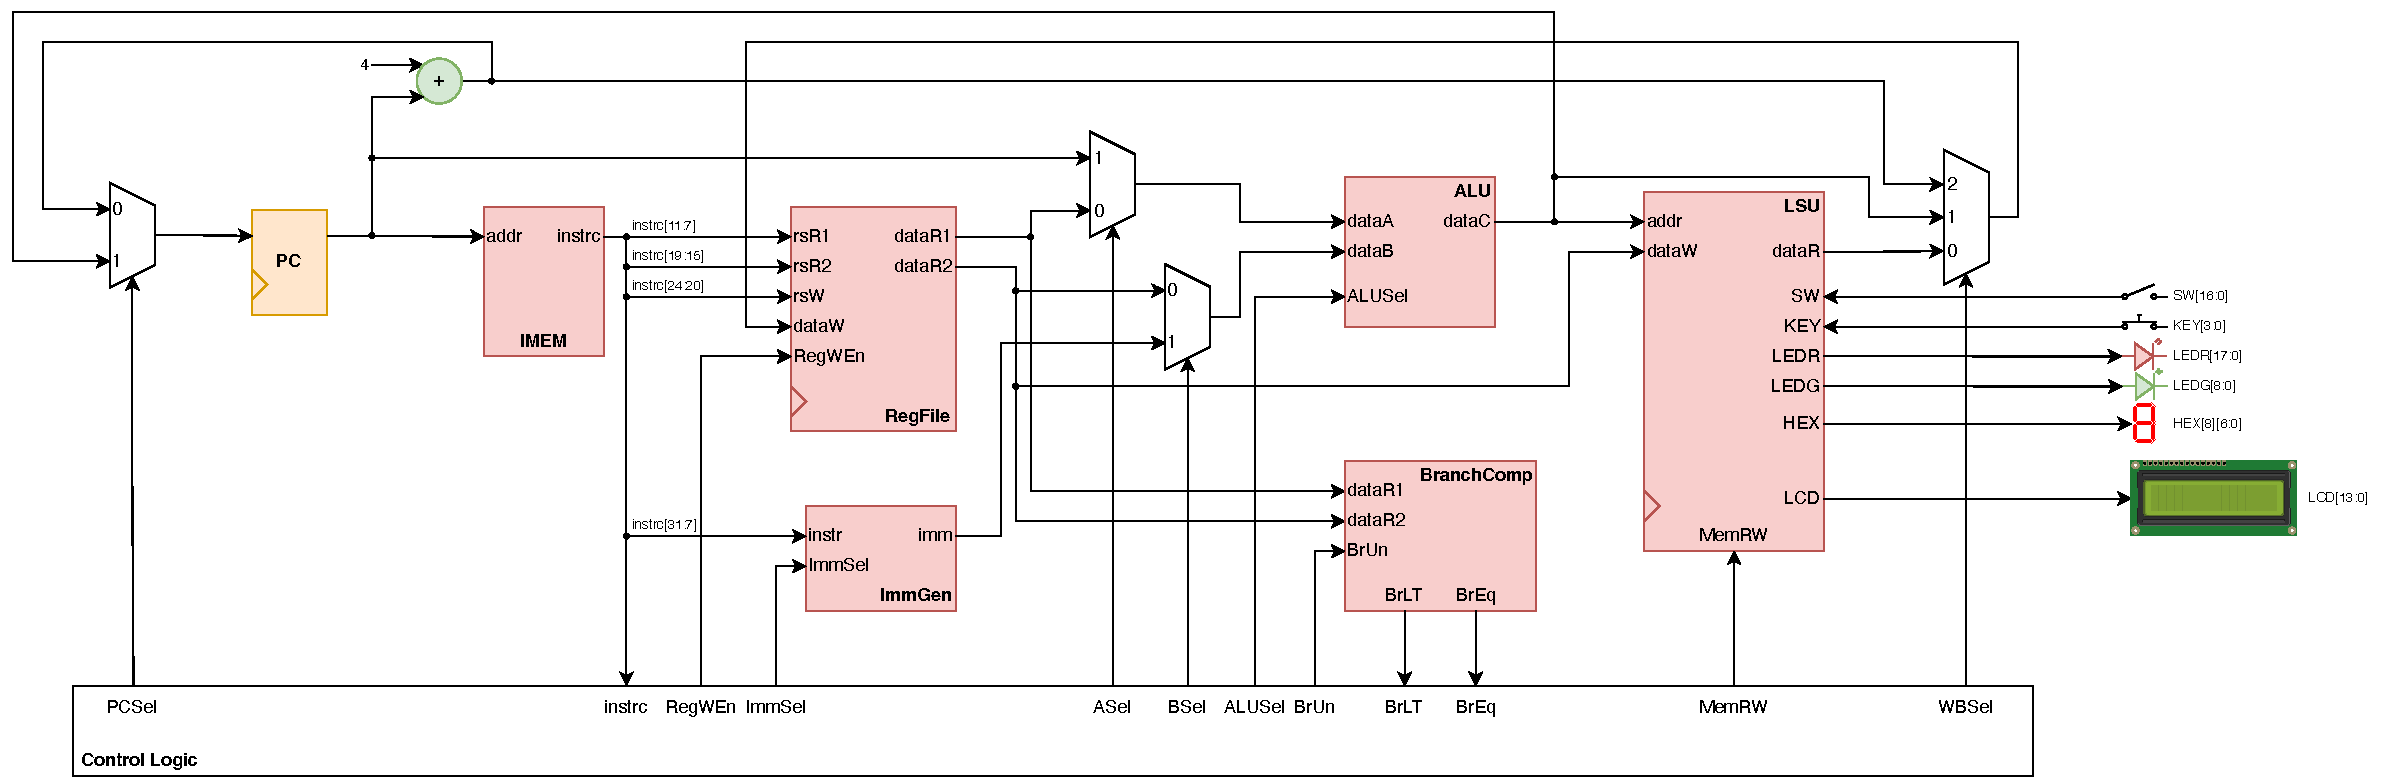
\includegraphics[scale=.6]{images/top_diagram.pdf}
    \caption{Top Module Diagram}
\end{figure}
\end{landscape}

\section{Register File}
The Register File in the RISC-V architecture typically consists of 32 registers, indexed from \texttt{x0} to \texttt{x31}. Register \texttt{x0} is typically referred to as the zero register and is hardwired to the value zero, meaning any write operation to \texttt{x0} will not have any effect on its value. In addition to this, \texttt{x0} is usually read-only, and any write operation to it does not alter its content. However, for the remaining registers (\texttt{x1} to \texttt{x31}), write operations are allowed and will update the values stored in those registers.

\begin{figure}[H]
    \centering
    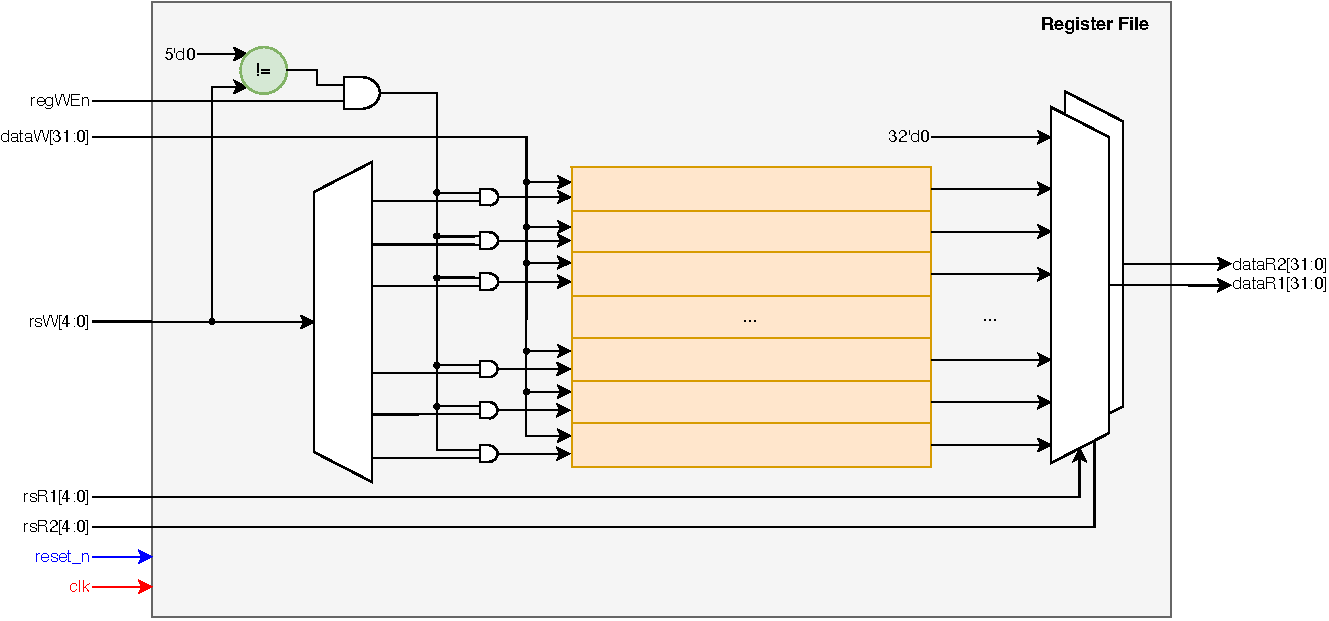
\includegraphics[width=\textwidth]{images/regfile.pdf}
    \caption{Register File Block Diagram}
\end{figure}

\section{Arithmetic Logic Unit}
In the RISC-V (Reduced Instruction Set Computer - Five) architecture, an ALU (Arithmetic Logic Unit) is a fundamental component responsible for performing arithmetic and bitwise operations on binary data. The ALU is responsible for executing various operations such as addition, subtraction, bitwise XOR, bitwise AND, bitwise OR, set less than, set less than unsigned, shift left logical, shift right logical, and shift right arithmetic.

The RISC-V ALU typically operates on fixed-length binary data, which is typically 32 bits or 64 bits depending on the specific RISC-V implementation. It takes input operands from the CPU's registers, performs the specified operation, and stores the result back into a register.

The ALU executes instructions of different types, including R-type and I-type instructions.
\begin{itemize}
    \item \texttt {R-type} instructions in RISC-V are used for arithmetic and bitwise operations that involve registers. In \texttt {R-type} instructions, the ALU performs the specified operation on the values in \texttt{rs1} and \texttt{rs2} and stores the result in \texttt{rd}.
    \item \texttt{I-type} instructions in RISC-V are used for immediate operations where one operand is an immediate value, typically a constant or a small value. In \texttt{I-type} instructions, the ALU performs the specified operation between the value in \texttt{rs1} and the immediate value \texttt{imm}, and stores the result in \texttt{rd}.
\end{itemize}

\begin{table}[H]
\centering
\caption{The operations of an RV32I ALU}
\begin{tabular}{|c|c|c|c|}
\hline
\textbf{Opcode} & \textbf{alu\_op} & \textbf{R-type}          & \textbf{I-type}            \\ \hline
0000            & ADD             & rd = rs1 + rs2           & rd = rs1 + imm             \\ \hline
1000            & SUB             & rd = rs1 - rs2           & N/A                        \\ \hline
0010            & SLT             & rd = (rs1 $<$ rs2) ? 1 : 0 & rd = (rs1 $<$ imm)  ?  1 : 0 \\ \hline
0011            & SLTU            & rd = (rs1 $<$ rs2) ? 1 : 0 & rd = (rs1 $<$ imm)  ?  1 : 0 \\ \hline
0100            & XOR             & rd = rs1 $\oplus$ rs2           & rd = rs1 $\oplus$ imm             \\ \hline
0110            & OR              & rd = rs1 $\vee$ rs2           & rd = rs1 $\vee$ imm             \\ \hline
0111            & AND             & rd = rs1 $\wedge$ rs2           & rd = rs1 $\wedge$  imm             \\ \hline
0001            & SLL             & rd = rs1 $\ll$ rs2 [4:0]    & rd = rs1 $\ll$ imm [4:0]      \\ \hline
0101            & SRL             & rd = rs1 $\gg$ rs2 [4:0]    & rd = rs1 $\gg$ imm [4:0]      \\ \hline
1101            & SRA             & rd = rs1 $\ggg$ rs2 [4:0]   & rd = rs1 $\ggg$ imm [4:0]     \\ \hline
1001            & B            & rs2                      & rs2                        \\ \hline
\end{tabular}
\end{table}
The purpose of adding opcodes to establish a truth table is to determine the behavior of \texttt{unsigned\_sel} and \texttt{neg\_sel} operations. These opcodes are used to perform selection and negation operations on unsigned values in a digital system. By creating a truth table, we can systematically analyze and define the output values of these operations based on different input combinations.

\begin{table}[H]
\centering
\caption{Truth table for \texttt{unsigned\_sel} and \texttt{neg\_sel} signals}
\label{alu}
\begin{tabular}{|c|c|c|c|}
\hline
\textbf{Operation} & \textbf{alu\_op} & \textbf{neg\_sel} & \textbf{unsigned\_sel} \\ \hline
ADD                & 0000          & 0                & 0                     \\ \hline
SLL                & 0001          & X                & X                     \\ \hline
SLT                & 0010          & 1                & 0                     \\ \hline
SLTU               & 0011          & 1                & 1                     \\ \hline
XOR                & 0100          & X                & X                     \\ \hline
SRL                & 0101          & X                & X                     \\ \hline
OR                 & 0110          & X                & X                     \\ \hline
AND                & 0111          & X                & X                     \\ \hline
SUB                & 1000          & 1                & 0                     \\ \hline
N/A                & 1001          & X                & X                     \\ \hline
N/A                & 1010          & X                & X                     \\ \hline
N/A                & 1011          & X                & X                     \\ \hline
N/A                & 1100          & X                & X                     \\ \hline
SRA                & 1101          & X                & X                     \\ \hline
N/A                & 1110          & X                & X                     \\ \hline
N/A                & 1111          & X                & X                     \\ \hline
\end{tabular}
\end{table}

Then we use the K-map to given the output of \texttt{unsigned\_sel} and \texttt{neg\_sel}

\begin{figure}[H]
    \centering
    \subfloat[The K-map for \texttt{neg\_sel}]{\begin{karnaugh-map}[4][4][1] [$D$][$C$][$B$][$A$]
  \minterms{2,3,8}
  \indeterminants{1,4,5,6,7,9,10,11,12,13,14,15}
  \autoterms[0]
  \implicant{12}{10}
  \implicant{3}{10}
\end{karnaugh-map}}
    \subfloat[The K-map for \texttt{unsigned\_sel}]{\begin{karnaugh-map}[4][4][1] [$D$][$C$][$B$][$A$]
  \minterms{3}
  \indeterminants{1,4,5,6,7,9,10,11,12,13,14,15}
  \autoterms[0]
  \implicant{1}{11}
\end{karnaugh-map}}
\caption{Karnaugh Map for simplifying \texttt{neg\_sel} and \texttt{unsigned\_sel}}
\end{figure}

% \begin{figure}[H]
%     \centering
%     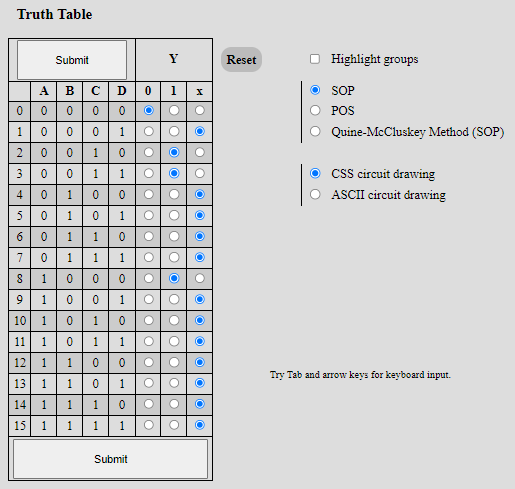
\includegraphics[width=.8\textwidth]{images/2_Sel.png}
%     \caption{Truth table for \texttt{neg\_sel}}
% \end{figure}

%  \begin{figure}[H]
%     \begin{center}
%     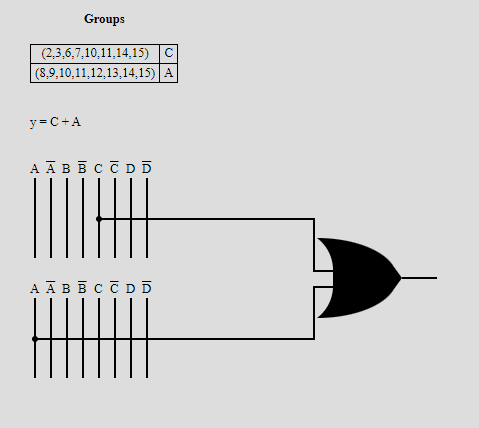
\includegraphics[trim=0cm 0cm 0cm 2.5cm,clip,width=.80\textwidth]{images/2_Sel_1.png}
%     \caption{The output of \texttt{neg\_sel}}
%     \end{center}
% \end{figure}

%  \begin{figure}[H]
%     \begin{center}
%     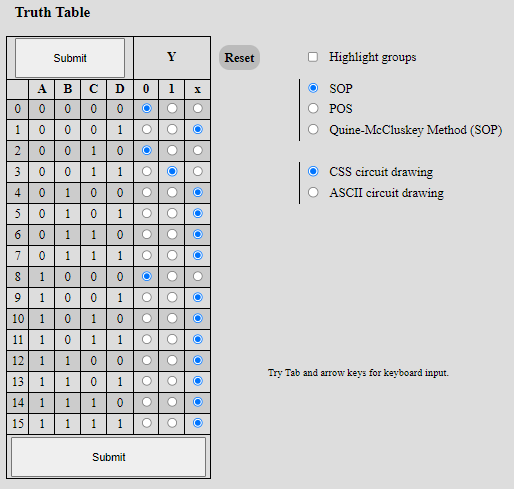
\includegraphics[trim=0cm 0cm 0cm 0cm,clip,width=.80\textwidth]{images/un.png}
%     \caption{Truth table for \texttt{unsigned\_sel}}
%     \end{center}
% \end{figure}

% \begin{figure}[H]
%     \centering
%     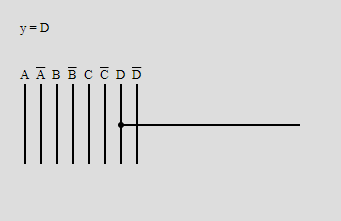
\includegraphics[width=.8\textwidth]{images/un_!.png}
%     \caption{The output of \texttt{unsigned\_sel}}
% \end{figure}

% The \texttt{add\_sub\_less} module is a component in designing an Arithmetic Logic Unit, \texttt{add\_sub\_less} that performs addition, subtraction operations. This module is designed to select between addition and subtraction based on a control signal (\texttt{neg\_sel}) and the the number is signed or unsigned by \texttt{unsigned\_sel} signal. The module takes two input operands, a control signal for operation selection (\texttt{neg\_sel}), and the signed or unsigned number by \texttt{unsigned\_sel} signal. When the \texttt{neg\_sel} ísignal is \texttt{0}, it indicates an addition operation. In this case, the module performs the addition of the two operands and generates a 32-bit result. This result represents the outcome of the addition operation, then the same when \texttt{neg\_sel} signal is \texttt{1} (the subtraction operation). At the output, the module separates the result into a 32-bit \texttt{result} output and a 1-bit \texttt{less\_than} signal. The 1-bit \texttt{less\_than} signal is concatenated with 30-bit \texttt{0} MSB, then it is the result of \texttt{sltu, slt}.

The \texttt{add\_sub\_less} module within the Arithmetic Logic Unit (ALU) plays a crucial role in performing addition and subtraction operations while also generating a 1-bit signal to indicate whether input A is less than input B. Addition is a straightforward operation, but subtraction is executed by adding input A to the two's complement of input B. The \texttt{less\_than} signal is derived from the overflow bit resulting from the subtraction operation.

This module takes two inputs, A and B, as well as control signals \texttt{neg\_sel} and \texttt{unsigned\_sel}. The \texttt{neg\_sel} signal is set to 1 when the opcode corresponds to subtraction (\texttt{sub}), set less than (\texttt{slt}), or set less than unsigned (\texttt{sltu}) instructions, as these involve subtraction. The \texttt{unsigned\_sel} signal is set to 1 specifically for the \texttt{sltu} operation.

A key aspect of this operation is the signed extension of inputs A and B to 33 bits if \texttt{unsigned\_sel} is 0, and zero padding if \texttt{unsigned\_sel} is 1. During the subtraction, if the result is negative, which is indicated by bit 32 (the overflow bit) being set to 1, it indicates that A is indeed less than B. This mechanism enables the ALU to efficiently handle addition, subtraction, and the less-than comparison in a systematic manner.

 \begin{figure}[H]
    \begin{center}
    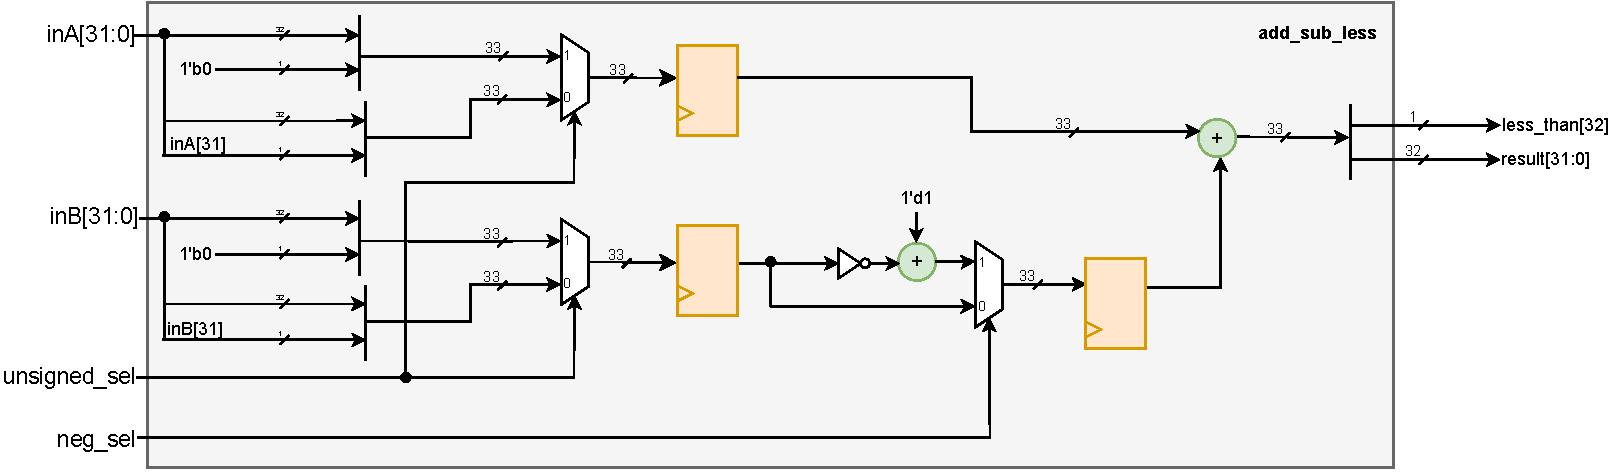
\includegraphics[trim=0cm 0cm 0cm 0cm,clip,width=\textwidth]{images/addsub.pdf}
    \caption{The design of \texttt{add\_sub\_less} module}
    \end{center}
\end{figure}
After building the \texttt{addsub} module, we conduct to integrate the  \texttt{addsub} module in to the ALU, the result of various operations, including \texttt{xor}, \texttt{or}, \texttt{and}, \texttt{sll} (left logical shift), \texttt{srl} (right logical shift), and \texttt{sra} (right arithmetic shift), will be determined by the \texttt{sel} signal originating from the control unit module.
 \begin{figure}[H]
    \begin{center}
    
\includegraphics[trim=0cm 0cm 0cm 0cm,clip,width=.90\textwidth]{images/alu}
    \caption{The design of \texttt{alu} module}
    \end{center}
\end{figure}

\section{Branch Comparision}
 \begin{figure}[H]
    \begin{center}
    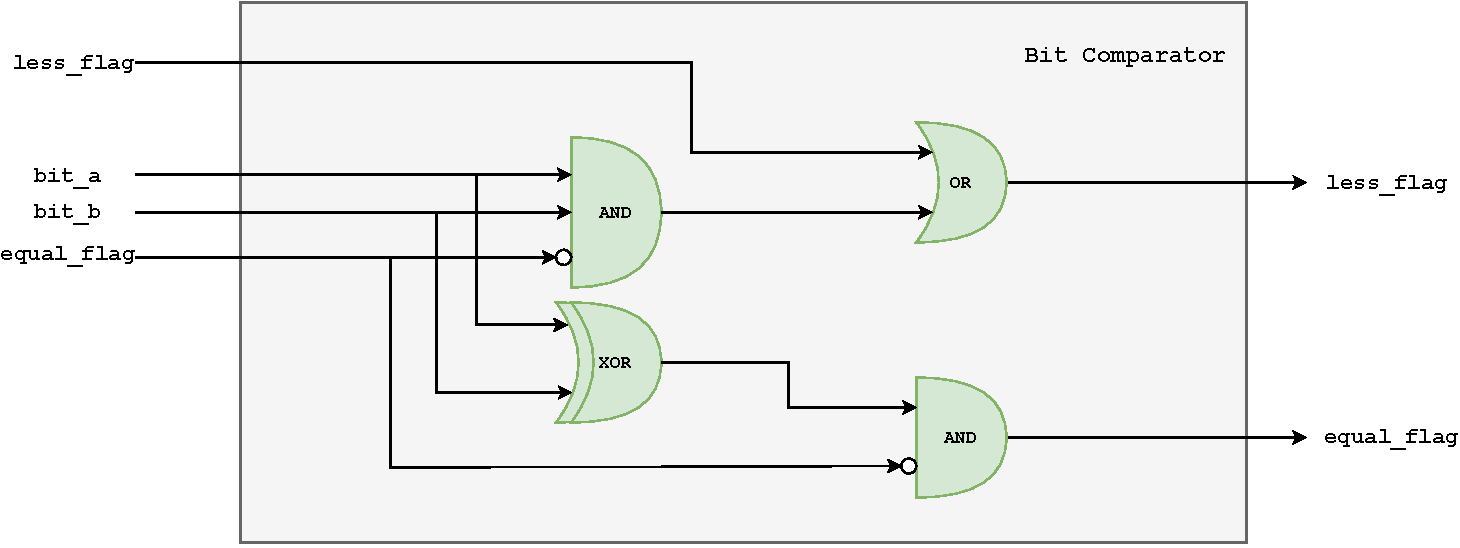
\includegraphics[trim=0cm 0cm 0cm 0cm,clip,width=.90\textwidth]{images/milestone2-bitcomp.drawio-1.pdf}
    \caption{The design of simple logic bit comparator}
    \end{center}
\end{figure}

 \begin{figure}[H]
    \begin{center}
    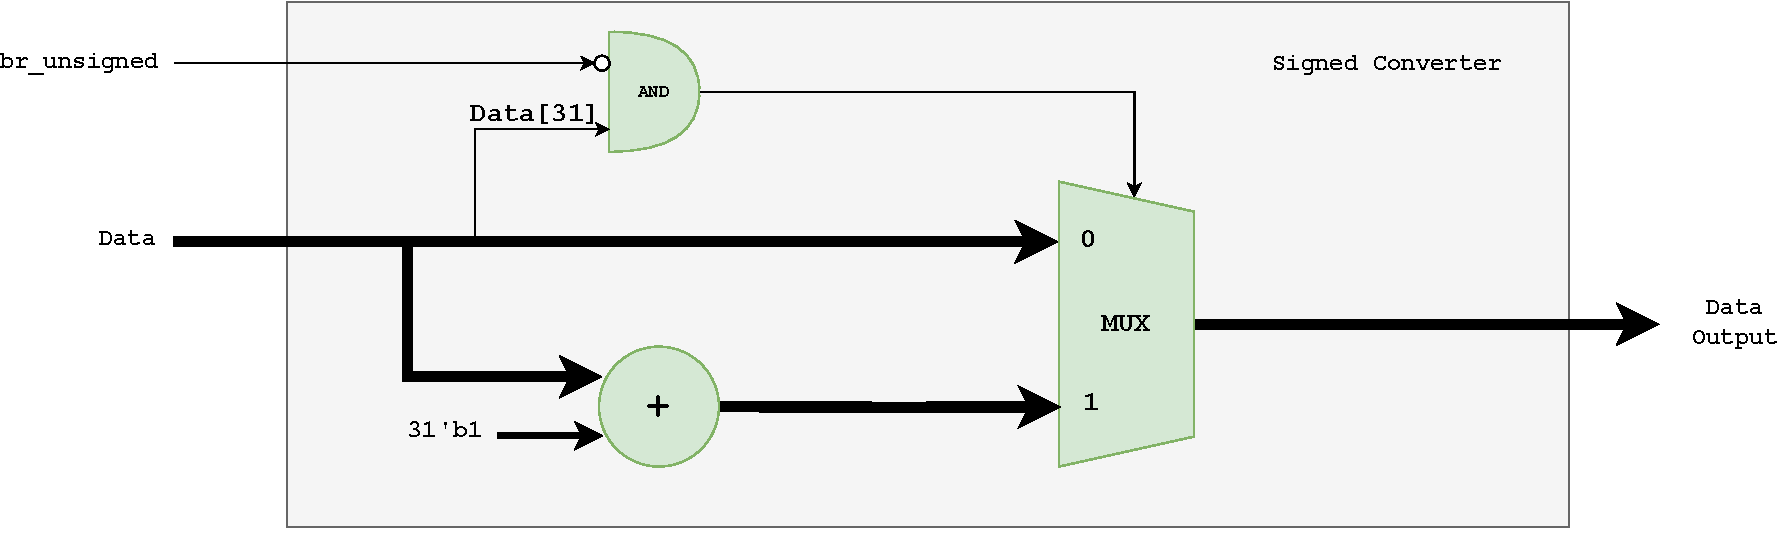
\includegraphics[trim=0cm 0cm 0cm 0cm,clip,width=.90\textwidth]{images/milestone2-signcvter.drawio.pdf}
    \caption{The design of  2’s complement 32-bit converter}
    \end{center}
\end{figure}

The branch comparator, relies on the functionality of two core modules: the bit comparator and the sign converter. The bit comparator handles the intricate task of comparing individual bits in the inputs, \texttt{rs1\_data} and \texttt{rs2\_data}, while considering the prior comparison results indicated by \texttt{in\_less} and \texttt{in\_equal} for higher bits. Its primary goal is to produce two one-bit outputs, \texttt{out\_less} and \texttt{out\_equal}, which signify whether \texttt{rs1\_data} is less than or equal to \texttt{rs2\_data}, respectively. This is achieved through a clever combination of XOR and AND gates, meticulously designed to perform the bit-by-bit comparisons effectively.

On the other hand, the sign converter plays a crucial role in processing 32-bit inputs, either  \texttt{rs1\_data} or  \texttt{rs2\_data}, by considering the context of signed or unsigned comparisons, as indicated by the \texttt{br\_unsigned} signal. It delivers 32-bit outputs, \texttt{data\_r1} or  \texttt{data\_r2}, reflecting the converted values based on the input and the selected mode. The sign converter leverages a multiplexer to make the choice between preserving the original value and applying a two's complement transformation, depending on the sign bit and the\texttt{br\_unsigned} signal. This operation is facilitated through a combination of NOT gates and an adder, ensuring an accurate representation of the converted data
 \begin{figure}[H]
    \centering
    \begin{center}
    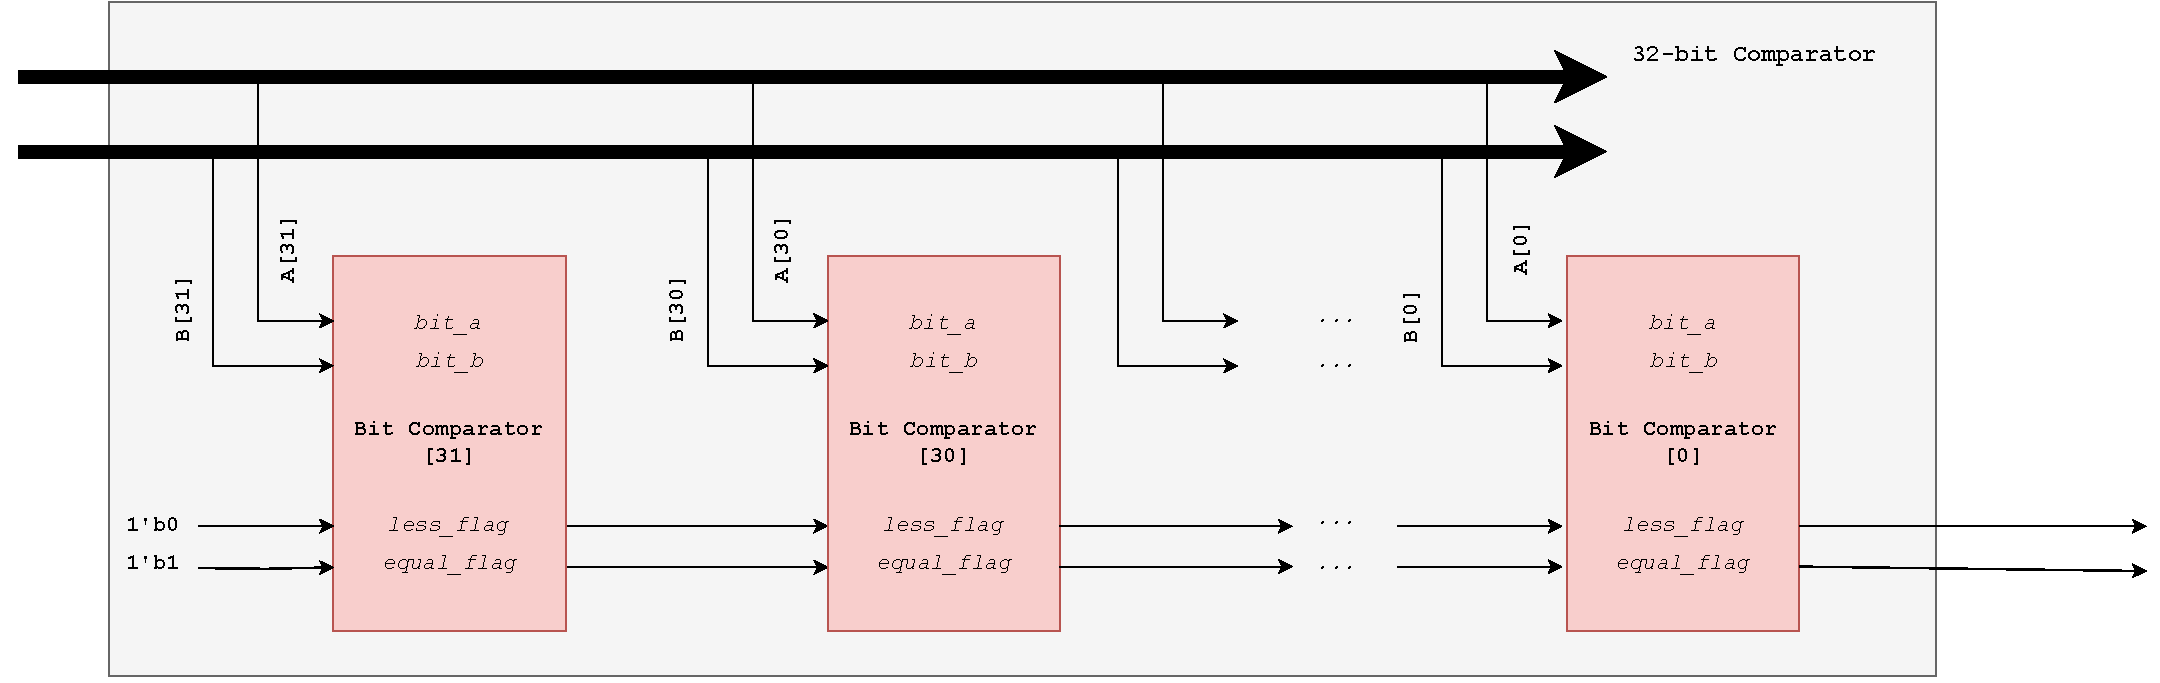
\includegraphics[trim=0cm 0cm 0cm 0cm,clip,width=\textwidth]{images/milestone2-regcomp.drawio.pdf}
    \caption{Structural Desciption of A typical 32-bit comparator using bitcomp IP}
    \end{center}
\end{figure}

The bit comparator's intrinsic capability to compare a single bit necessitates the use of 32 such comparators in the context of the RISC-V CPU, arranged in a sequential series. A noteworthy aspect of this arrangement is that the 31st bit comparator must be linked to the ``equal''and ``less'' inputs with values 1 and 0, respectively, a design choice that assumes any 33rd bit not within the defined 32-bit range is considered equal. This precision ensures a meticulous comparison of the two data sets. The resulting output flag signals are interconnected in a series and serve as inputs for the subsequent module, collectively contributing to the creation of a conventional 32-bit comparator. The provided code within the \texttt{regcomp} module effectively captures this concept through a \texttt{generate} loop, wherein bit comparators are instantiated and interconnected to enable precise 32-bit comparisons.
 \begin{figure}[H]
    \begin{center}
    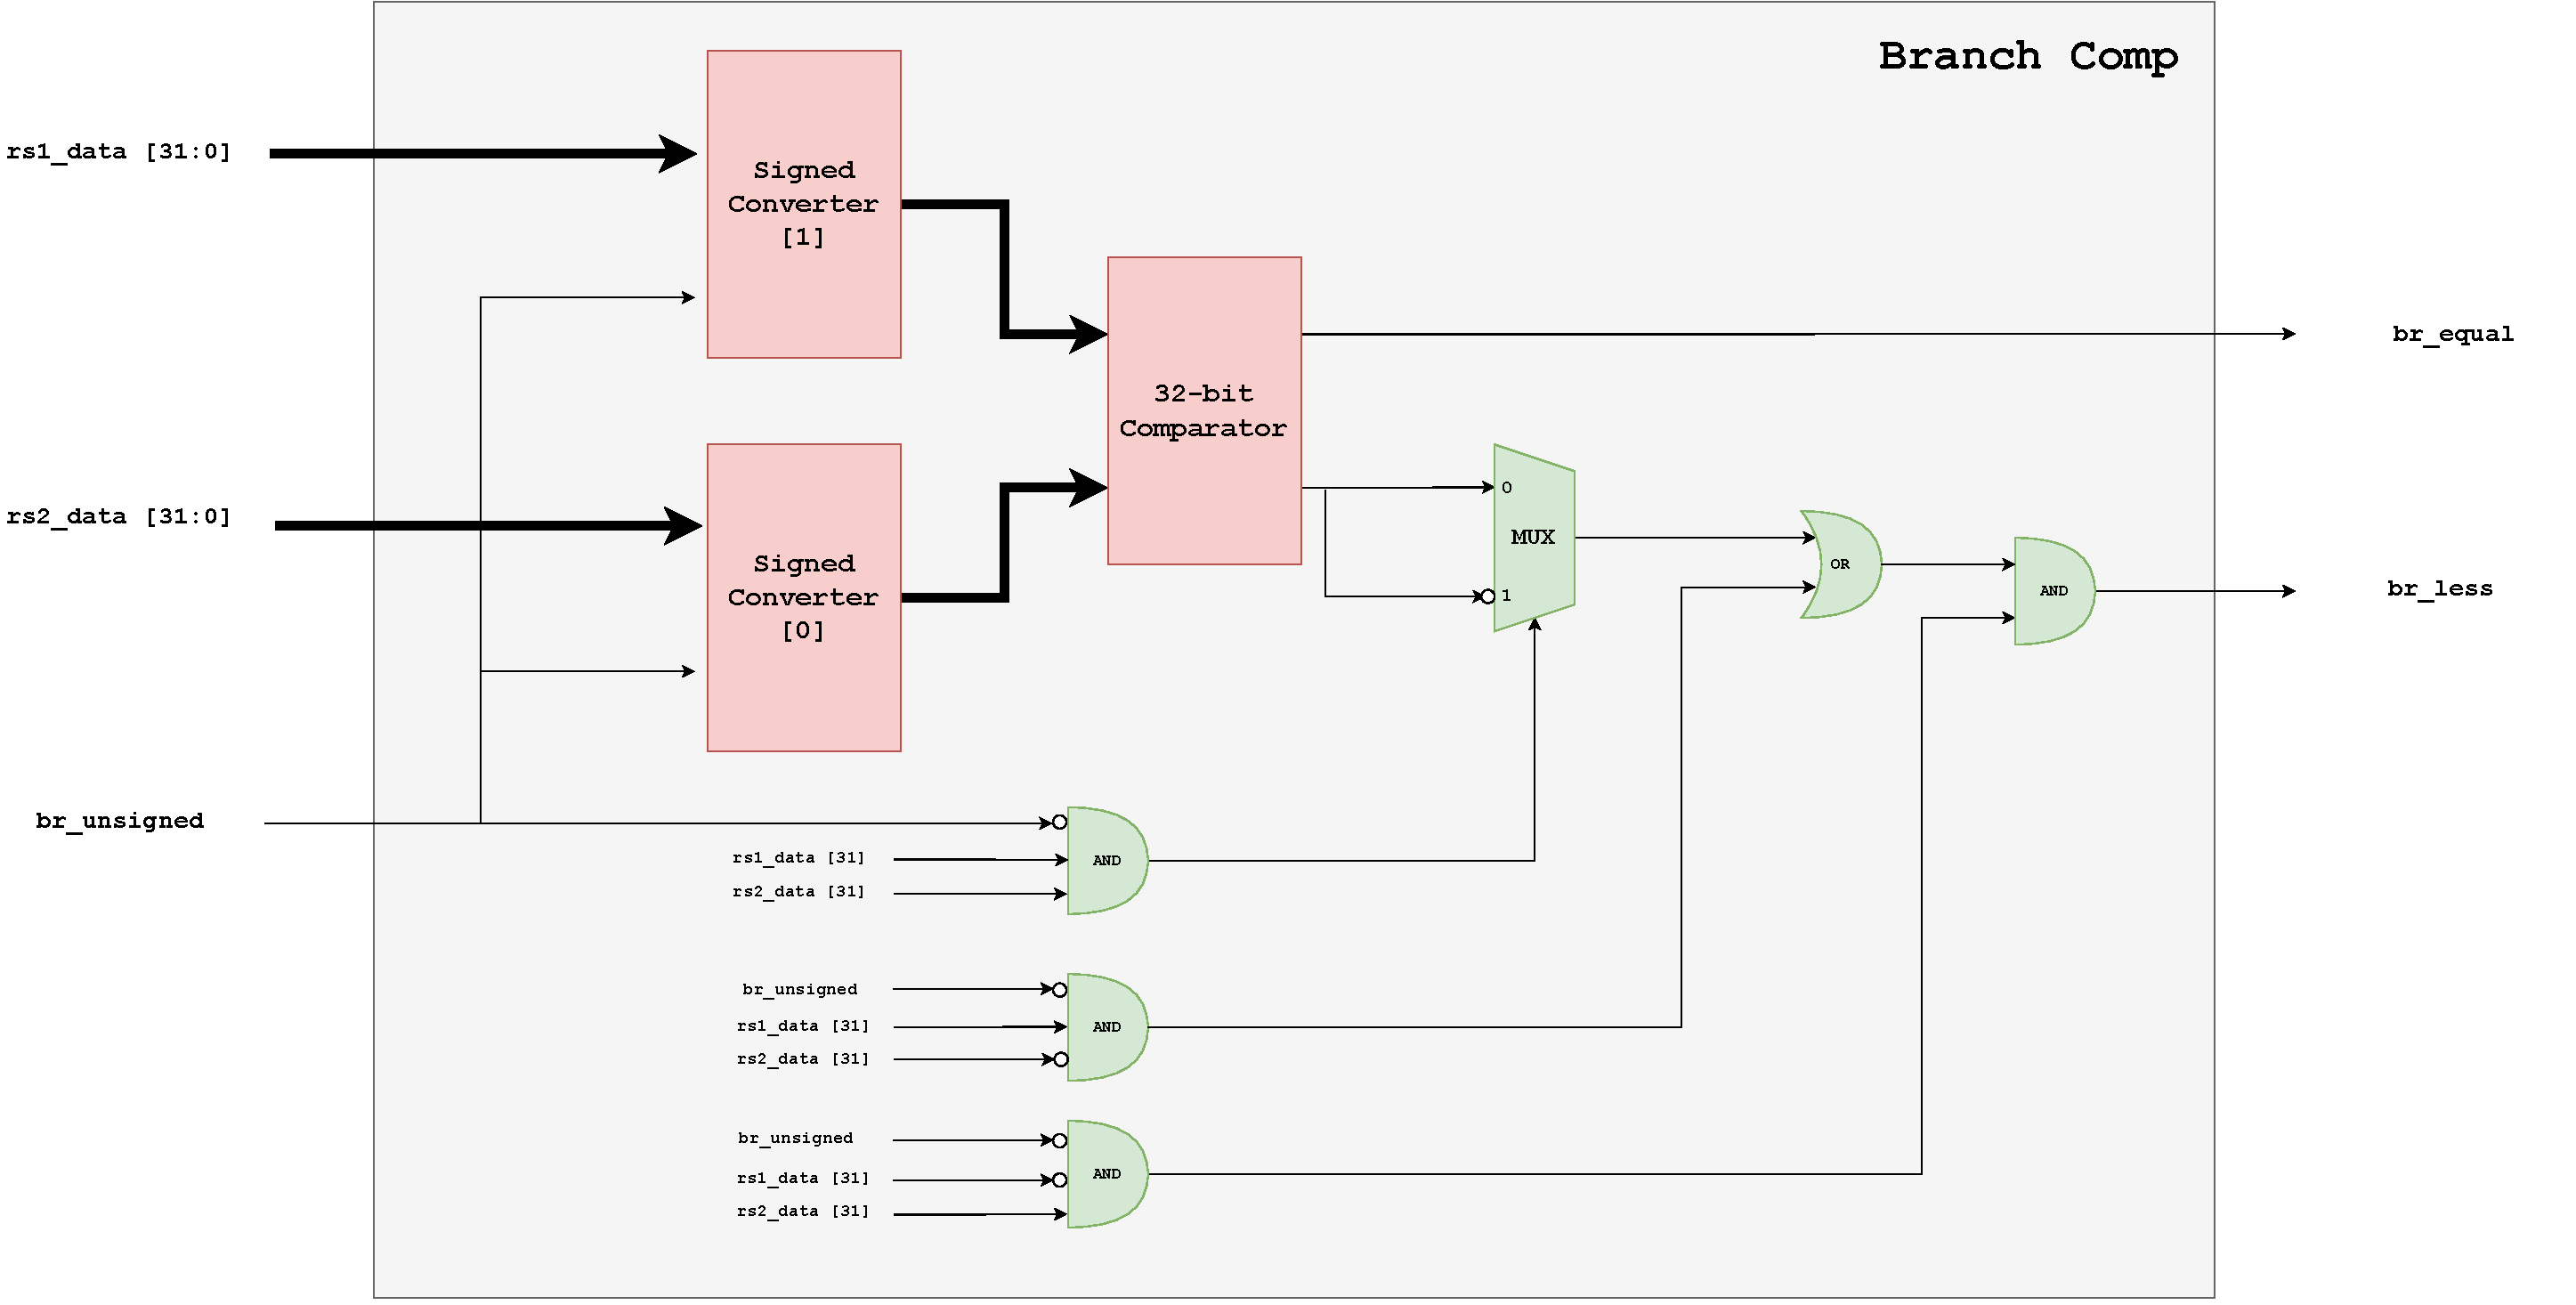
\includegraphics[trim=0cm 0cm 0cm 0cm,clip,width=\textwidth]{images/milestone2-brcomp.drawio.pdf}
    \caption{The top-level architecture of RISCV Branch Comparator Unit}
    \end{center}
\end{figure}
The apex of the branch comparator's design is represented by its top-level architecture, an integral component of the Execution stage within a single-cycle RISC-V CPU. This branch comparator encompasses key input ports, namely  \texttt{rs1\_data}, \texttt{rs2\_data}, and \texttt{br\_unsigned}, while yielding crucial output ports in the form of \texttt{br\_less} and \texttt{br\_equal}. The architectural illustration portrays the interconnection of two sign converters, each receiving data from one of the input ports, and subsequently feeding this processed data into two 32-bit comparators. This configuration lays the foundation for the branch comparator's core structure. However, it introduces a notable challenge, centered around controlling the \texttt{less} signal under distinct conditions for both unsigned and signed comparisons. Unsigned comparisons adhere to a straightforward design, as seen in the former architecture. Conversely, signed comparisons give rise to three distinct scenarios. To present these cases systematically, a table could be constructed, outlining the conditions and their corresponding outcomes. Notably, the 31st bit, which also serves as the signed bit, undergoes meticulous processing through a logic combination circuit, ensuring the precise generation of the \texttt{less} signal across all scenarios.
\begin{table}[H]
\centering
\caption{Comparison Strategies for two signed 32-bit number}
\begin{tabular}{|c|c|c|}
\hline
\textbf{rs1[31]} & \textbf{rs2[31]} & \textbf{Compare Flag}                       \\ \hline
negative 1’s     & negative 1’s     & Convert data   and complement 'less' output \\ \hline
negative 1’s     & positive 0’s     & 'Less' is   immediately set to 'on'         \\ \hline
positive 0’s     & negative 1’s     & 'Less' is immediately   set to 'off'        \\ \hline
\end{tabular}
\end{table}

\begin{landscape}
\section{Immediate Generator}
 \begin{figure}[H]
    \begin{center}
    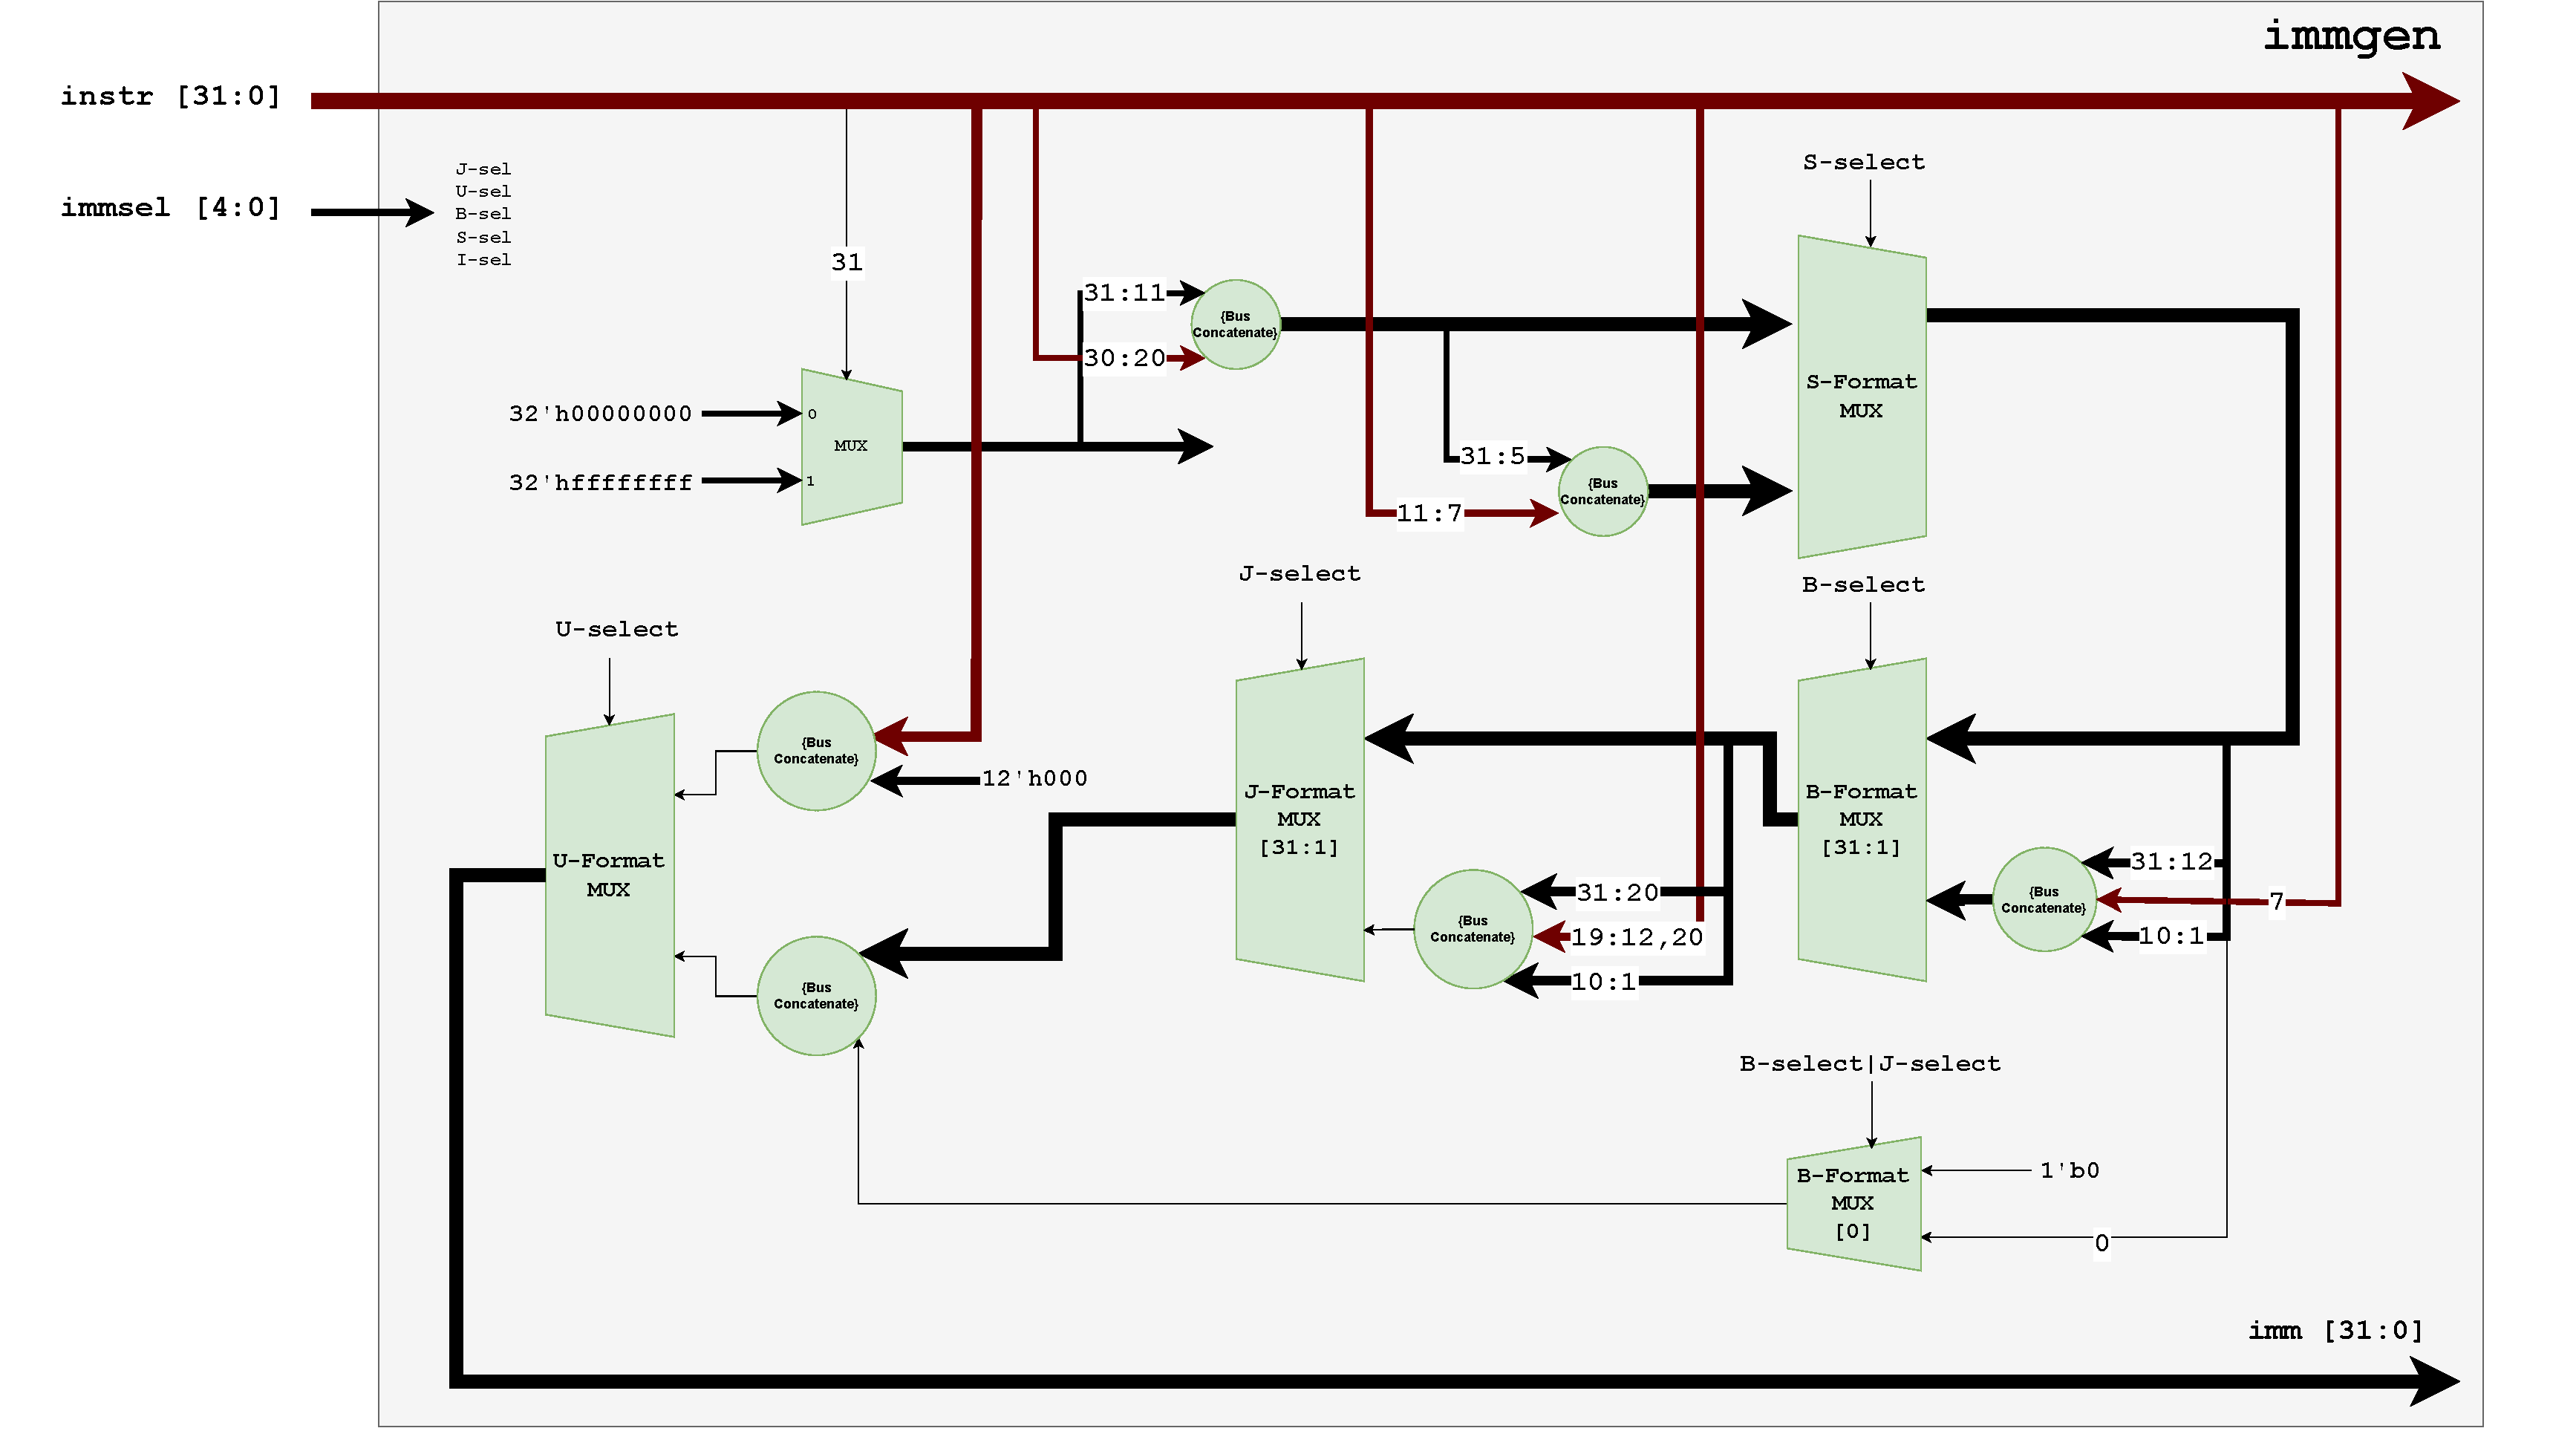
\includegraphics[width=1.5\textwidth]{images/milestone2-immgen.drawio.pdf}
    \caption{A design of immediate generator, usingmultiplexer}
    \end{center}
\end{figure}
\end{landscape}

The implementation of the immediate generator is a critical component in the design of a RISC-V CPU, responsible for arranging the bits or bytes of instructions to form the appropriate immediate values. In the RISC-V format, there are various types of immediates, including I, B, S, J, and U formats, which require the use of multiplexers to direct the wiring order of the bus. The figure illustrates a design that guides the bus of immediates for these different formats. The I-format serves as the starting point, requiring minimal sign extension and acting as a reference for subsequent stages. The S-stage, identified by a MUX, transforms the bus into an S-type immediate, distinct from the I-type. Similar approaches are applied to B-type masking over S-type and J-type masking over J-type, with special note taken for the commonality of the last bits in J and B types, which are handled separately to reduce the need for additional MUXes. The U-type is entirely different from the others, and the chosen mechanism is applied to determine whether it is a U-type or part of the multi-stage ISBJ formats. The selection of the immediate bus path is governed by the \texttt{imm\_sel} port, which is protocol decoded in a one-hot format with 5 bits, ensuring precise and effective control of immediate generation.

The instruction 32 bit in Single Cycle RISCV CPU is composed of different fields that encode the operation, the operands and the destination of the result. One of these fields is the bit that, which indicates whether the instruction is an immediate or a register instruction. The table below shows some summary of how the bit that affects the generation of immediate values from the instruction 32 bit in Single Cycle RISCV CPU.

\begin{table}[H]
\centering
\caption{The formation of immediate from system verilog implementation}
\begin{tabular}{|c|l|}
\hline
\textbf{Immediate   format} & \textbf{Bit   Extraction}                              \\ \hline
I-type                      & \texttt{\{signxt[31:11],instr[30:20]\}}                           \\ \hline
S-type                      & \texttt{\{Itype[31:5],instr[11:7]\}}                              \\ \hline
B-type                      & \texttt{\{Stype[31:12],instr[7],Stype[10:1],1'b0\}}               \\ \hline
U-type                      & \texttt{\{instr[31:12],12'd0\}}                                   \\ \hline
J-type                      & \texttt{\{Btype[31:20],instr[19:12],instr[20],Btype[10:1],1'b0\}} \\ \hline
\end{tabular}
\end{table}

\begin{landscape}
\section{Control Unit}
\begin{table}[H]
    \centering
    \caption{Control Unit Truth Table}
    \label{ctrl_unit}
\resizebox{\columnwidth}{!}{% <------ Don't forget this %
\begin{tabular}{|c|c|c|c|c|c|c|c|c|c|c|c|c|c|c|c|c|}
\hline
                         & opcode & inst[6:2] & inst[14:12] & inst[30] & BrEq & BrLT & PCSel & ImmSel  & BrUn & Asel & Bsel & ALUSel & MemRW & RegWEn & WBSel & LdStSel \\ \hline
\multirow{10}{*}{R-type} & add    & 01100     & 000         & 0        & ~    & ~    & 0     & ~       & ~    & 0    & 0    & 0000   & 0     & 1      & 01    & ~       \\ \cline{2-17} 
                         & sub    & 01100     & 000         & 1        & ~    & ~    & 0     & ~       & ~    & 0    & 0    & 1000   & 0     & 1      & 01    & ~       \\ \cline{2-17} 
                         & xor    & 01100     & 100         & 0        & ~    & ~    & 0     & ~       & ~    & 0    & 0    & 0100   & 0     & 1      & 01    & ~       \\ \cline{2-17} 
                         & or     & 01100     & 110         & 0        & ~    & ~    & 0     & ~       & ~    & 0    & 0    & 0110   & 0     & 1      & 01    & ~       \\ \cline{2-17} 
                         & and    & 01100     & 111         & 0        & ~    & ~    & 0     & ~       & ~    & 0    & 0    & 0111   & 0     & 1      & 01    & ~       \\ \cline{2-17} 
                         & sll    & 01100     & 001         & 0        & ~    & ~    & 0     & ~       & ~    & 0    & 0    & 0001   & 0     & 1      & 01    & ~       \\ \cline{2-17} 
                         & srl    & 01100     & 101         & 0        & ~    & ~    & 0     & ~       & ~    & 0    & 0    & 0101   & 0     & 1      & 01    & ~       \\ \cline{2-17} 
                         & sra    & 01100     & 101         & 1        & ~    & ~    & 0     & ~       & ~    & 0    & 0    & 1101   & 0     & 1      & 01    & ~       \\ \cline{2-17} 
                         & slt    & 01100     & 010         & 0        & ~    & ~    & 0     & ~       & ~    & 0    & 0    & 0010   & 0     & 1      & 01    & ~       \\ \cline{2-17} 
                         & sltu   & 01100     & 011         & 0        & ~    & ~    & 0     & ~       & ~    & 0    & 0    & 0011   & 0     & 1      & 01    & ~       \\ \hline
\multirow{14}{*}{I-type}  & addi   & 00100     & 000         & ~        & ~    & ~    & 0     & 00001 (I) & ~    & 0    & 1    & 0000   & 0     & 1      & 01    & ~       \\ \cline{2-17} 
                         & xori   & 00100     & 100         & ~        & ~    & ~    & 0     & 00001 (I) & ~    & 0    & 1    & 0100   & 0     & 1      & 01    & ~       \\ \cline{2-17} 
                         & ori    & 00100     & 110         & ~        & ~    & ~    & 0     & 00001 (I) & ~    & 0    & 1    & 0110   & 0     & 1      & 01    & ~       \\ \cline{2-17} 
                         & andi   & 00100     & 111         & ~        & ~    & ~    & 0     & 00001 (I) & ~    & 0    & 1    & 0111   & 0     & 1      & 01    & ~       \\ \cline{2-17} 
                         & slli   & 00100     & 001         & 0        & ~    & ~    & 0     & 00001 (I) & ~    & 0    & 1    & 0001   & 0     & 1      & 01    & ~       \\ \cline{2-17} 
                         & srli   & 00100     & 101         & 0        & ~    & ~    & 0     & 00001 (I) & ~    & 0    & 1    & 0101   & 0     & 1      & 01    & ~       \\ \cline{2-17} 
                         & srai   & 00100     & 101         & 1        & ~    & ~    & 0     & 00001 (I) & ~    & 0    & 1    & 1101   & 0     & 1      & 01    & ~       \\ \cline{2-17} 
                         & slti   & 00100     & 010         & ~        & ~    & ~    & 0     & 00001 (I) & ~    & 0    & 1    & 0010   & 0     & 1      & 01    & ~       \\ \cline{2-17} 
                         & sltiu  & 00100     & 011         & ~        & ~    & ~    & 0     & 00001 (I) & ~    & 0    & 1    & 0011   & 0     & 1      & 01    & ~       \\ \cline{2-17} 
                         & lb     & 00000     & 000         & ~        & ~    & ~    & 0     & 00001 (I) & ~    & 0    & 1    & 0000   & 0     & 1      & 00    & 000     \\ \cline{2-17} 
                         & lh     & 00000     & 001         & ~        & ~    & ~    & 0     & 00001 (I) & ~    & 0    & 1    & 0000   & 0     & 1      & 00    & 001     \\ \cline{2-17} 
                         & lw     & 00000     & 010         & ~        & ~    & ~    & 0     & 00001 (I) & ~    & 0    & 1    & 0000   & 0     & 1      & 00    & 010     \\ \cline{2-17} 
                         & lbu    & 00000     & 100         & ~        & ~    & ~    & 0     & 00001 (I) & ~    & 0    & 1    & 0000   & 0     & 1      & 00    & 100     \\ \cline{2-17} 
                         & lhu    & 00000     & 101         & ~        & ~    & ~    & 0     & 00001 (I) & ~    & 0    & 1    & 0000   & 0     & 1      & 00    & 101     \\ \hline
\multirow{3}{*}{S-type}  & sb     & 01000     & 000         & ~        & ~    & ~    & 0     & 00010 (S) & ~    & 0    & 1    & 0000   & 1     & 0      & ~     & 000     \\ \cline{2-17} 
                         & sh     & 01000     & 001         & ~        & ~    & ~    & 0     & 00010 (S) & ~    & 0    & 1    & 0000   & 1     & 0      & ~     & 001     \\ \cline{2-17} 
                         & sw     & 01000     & 010         & ~        & ~    & ~    & 0     & 00010 (S) & ~    & 0    & 1    & 0000   & 1     & 0      & ~     & 010     \\ \hline
\end{tabular}
}
\end{table}
\end{landscape}

\begin{landscape}
\begin{table}[H]
    \centering
\resizebox{\columnwidth}{!}{% <------ Don't forget this %
\begin{tabular}{|c|c|c|c|c|c|c|c|c|c|c|c|c|c|c|c|c|}
    \hline
                             & opcode & inst[6:2] & inst[14:12] & inst[30] & BrEq & BrLT & PCSel & ImmSel  & BrUn & Asel & Bsel & ALUSel & MemRW & RegWEn & WBSel & LdStSel \\ \hline
    \multirow{14}{*}{B-type} & beq    & 11000     & 000         & ~        & 0    & ~    & 0     & 00100 (B) & ~    & 1    & 1    & 0000   & 0     & 0      & ~     & ~       \\ \cline{2-17} 
                             & beq    & 11000     & 000         & ~        & 1    & ~    & 1     & 00100 (B) & ~    & 1    & 1    & 0000   & 0     & 0      & ~     & ~       \\ \cline{2-17} 
                             & bne    & 11000     & 001         & ~        & 0    & ~    & 1     & 00100 (B) & ~    & 1    & 1    & 0000   & 0     & 0      & ~     & ~       \\ \cline{2-17} 
                             & bne    & 11000     & 001         & ~        & 1    & ~    & 0     & 00100 (B) & ~    & 1    & 1    & 0000   & 0     & 0      & ~     & ~       \\ \cline{2-17} 
                             & blt    & 11000     & 100         & ~        & ~    & 1    & 1     & 00100 (B) & 0    & 1    & 1    & 0000   & 0     & 0      & ~     & ~       \\ \cline{2-17} 
                             & blt    & 11000     & 100         & ~        & ~    & 0    & 0     & 00100 (B) & 0    & 1    & 1    & 0000   & 0     & 0      & ~     & ~       \\ \cline{2-17} 
                             & bltu   & 11000     & 110         & ~        & ~    & 1    & 1     & 00100 (B) & 1    & 1    & 1    & 0000   & 0     & 0      & ~     & ~       \\ \cline{2-17} 
                             & bltu   & 11000     & 110         & ~        & ~    & 0    & 0     & 00100 (B) & 1    & 1    & 1    & 0000   & 0     & 0      & ~     & ~       \\ \cline{2-17} 
                             & bge    & 11000     & 101         & ~        & 1    & 0    & 1     & 00100 (B) & 0    & 1    & 1    & 0000   & 0     & 0      & ~     & ~       \\ \cline{2-17} 
                             & bge    & 11000     & 101         & ~        & 0    & 0    & 1     & 00100 (B) & 0    & 1    & 1    & 0000   & 0     & 0      & ~     & ~       \\ \cline{2-17} 
                             & bge    & 11000     & 101         & ~        & 0    & 1    & 0     & 00100 (B) & 0    & 1    & 1    & 0000   & 0     & 0      & ~     & ~       \\ \cline{2-17} 
                             & bgeu   & 11000     & 111         & ~        & 1    & 0    & 1     & 00100 (B) & 1    & 1    & 1    & 0000   & 0     & 0      & ~     & ~       \\ \cline{2-17} 
                             & bgeu   & 11000     & 111         & ~        & 0    & 0    & 1     & 00100 (B) & 1    & 1    & 1    & 0000   & 0     & 0      & ~     & ~       \\ \cline{2-17} 
                             & bgeu   & 11000     & 111         & ~        & 0    & 1    & 0     & 00100 (B) & 1    & 1    & 1    & 0000   & 0     & 0      & ~     & ~       \\ \hline
    J-type                   & jal    & 11011     & ~           & ~        & ~    & ~    & 1     & 10000 (J) & ~    & 1    & 1    & 0000   & 0     & 1      & 10    & ~       \\ \hline
    JI-type                  & jalr   & 11001     & ~           & ~        & ~    & ~    & 1     & 00001 (I) & ~    & 0    & 1    & 0000   & 0     & 1      & 10    & ~       \\ \hline
    \multirow{2}{*}{U-type}  & lui    & 01101     & ~           & ~        & ~    & ~    & 0     & 01000 (U) & ~    & ~    & 1    & 1001   & 0     & 1      & 01    & ~       \\ \cline{2-17} 
                             & auipc  & 00101     &             &          &      &      & 0     & 01000 (U) &      & 1    & 1    & 0000   & 0     & 1      & 01    &         \\ \hline
\end{tabular}
}
\end{table}

From the table, we can observe the following encoding patterns for different instruction types:
\begin{itemize}
    \item For R-type instructions, \texttt{inst[6:2] == 01100}.
    \item For I-type instructions, \texttt{inst[6:2] == 00100} or \texttt{00000}.
    \item For S-type instructions, the condition is \texttt{inst[6:2] == 01000}.
    \item For B-type instructions, the condition is \texttt{inst[6:2] == 11000}.
    \item For J-type instructions, the condition is \texttt{inst[6:2] == 11011}.
    \item For U-type instructions, the condition is \texttt{inst[6:2] == 01101} or \texttt{00101}.
    \item For JI-type instructions, the condition is \texttt{inst[6:2] == 11001}.
\end{itemize}
\end{landscape}

\subsection*{PCSel}
\texttt{PCSel} controls the program counter (PC) selection. It is set to 0 for sequential execution (PC + 4), and 1 for non-sequential jumps (PC + immediate). Specifically, \texttt{PCSel} is set to 1 for J-type, JI-type, or B-type instructions with a true branch condition, defined as \texttt{PCSel = Jtype | JItype | (Btype \& branchTrue)}.

The \texttt{branch\_true} signal is activated under the following conditions: it is true when the opcode is \texttt{beq} and the \texttt{BrEq} signal is true, or when the opcode is \texttt{bne} and \texttt{BrEq} is false, or when the opcode is \texttt{blt} and the \texttt{BrLT} signal is true, or when the opcode is \texttt{bge} and either \texttt{BrEq} is true or both \texttt{BrEq} and \texttt{BrLT} are false.

\subsection*{ImmSel}
\texttt{ImmSel} determines the immediate extension mode, which specifies how to correctly extend the immediate value based on the type of the instruction. Thus, \texttt{ImmSel = \{Jtype, Utype, Btype, Stype, Itype | JItype\}}.

\subsection*{BrUn}
\texttt{BrUn} is a signal used in the Branch Comparison module. It is set to 0 when the branch instruction is for signed comparison and is set to 1 when the branch instruction is for unsigned comparison. From the table, we observed that \texttt{inst[13]} is the bit for selecting unsigned mode in B-type instruction. Thus, \texttt{BrUn = inst[13]}.

\subsection*{ASel}
\texttt{ASel} selects the A-value input for the ALU. It's set to 0 for most instructions, using \texttt{rs1} from the Register File. However, for B-type, J-type, and U-type instructions, it's set to 1, indicating the selection of the program counter (PC). So, \texttt{ASel = Btype | Jtype | Utype}.

\subsection*{BSel}
\texttt{BSel} selects the B-value input for the ALU. When it's 0, it uses \texttt{rs2} from the Register File. In R-type instructions, \texttt{BSel} is 0. For all other instructions, \texttt{BSel} is 1, indicating the use of the immediate generator output. So, \texttt{BSel = \url{~Rtype}}.

\subsection*{MemRW}
\texttt{MemRW} enables writing to the data memory, specifically in the Load-Store Unit (LSU). It is only enabled for S-type instructions. So, \texttt{MemRW = Stype}.

\subsection*{RegWEn}
\texttt{RegWEn} is the enable signal for writing to the Register File. It allows write operations to the register file. It is active for most instruction types, except for S-type and B-type instructions, where it is not used for register file writing. So, \texttt{RegWEn =  \url{~Stype} \& \url{~Btype}}.

\subsection*{WBSel}
\texttt{WBSel} determines the data source for writing to the register file.
\begin{itemize}
    \item 00: Selects the output data from the Load-Store Unit (LSU).
    \item 01: Selects the output of the Arithmetic Logic Unit (ALU).
    \item 10: Selects the value of PC + 4, applicable for \texttt{jal} and \texttt{jalr} instructions.
    \item[$\Rightarrow$] \texttt{WBSel = Ltype ? 00 : (Jtype | JItype) ? 10 : 01}
\end{itemize}

\subsection*{ALUSel}
\texttt{ALUSel} is a dynamic selection signal based on instruction type, and its behavior is determined as follows:
\begin{itemize}
    \item For R-type instructions, it is determined by \texttt{\{inst[30], inst[14:12]\}}.
    \item For I-type instructions (excluding loads (Ltype)), if the instruction is a shift operator (\texttt{sll}, \texttt{srl}, \texttt{sra}), it is \texttt{\{inst[30], inst[14:12]\}}; otherwise, \texttt{\{0, inst[14:12]\}}.
    \item For the \texttt{lui} instruction, it is set to \texttt{1001}, forwarding the B-value.
    \item For all other instructions, it defaults to \texttt{0000}, indicating an addition operation.
\end{itemize}

\begin{figure}[H]
    \centering
    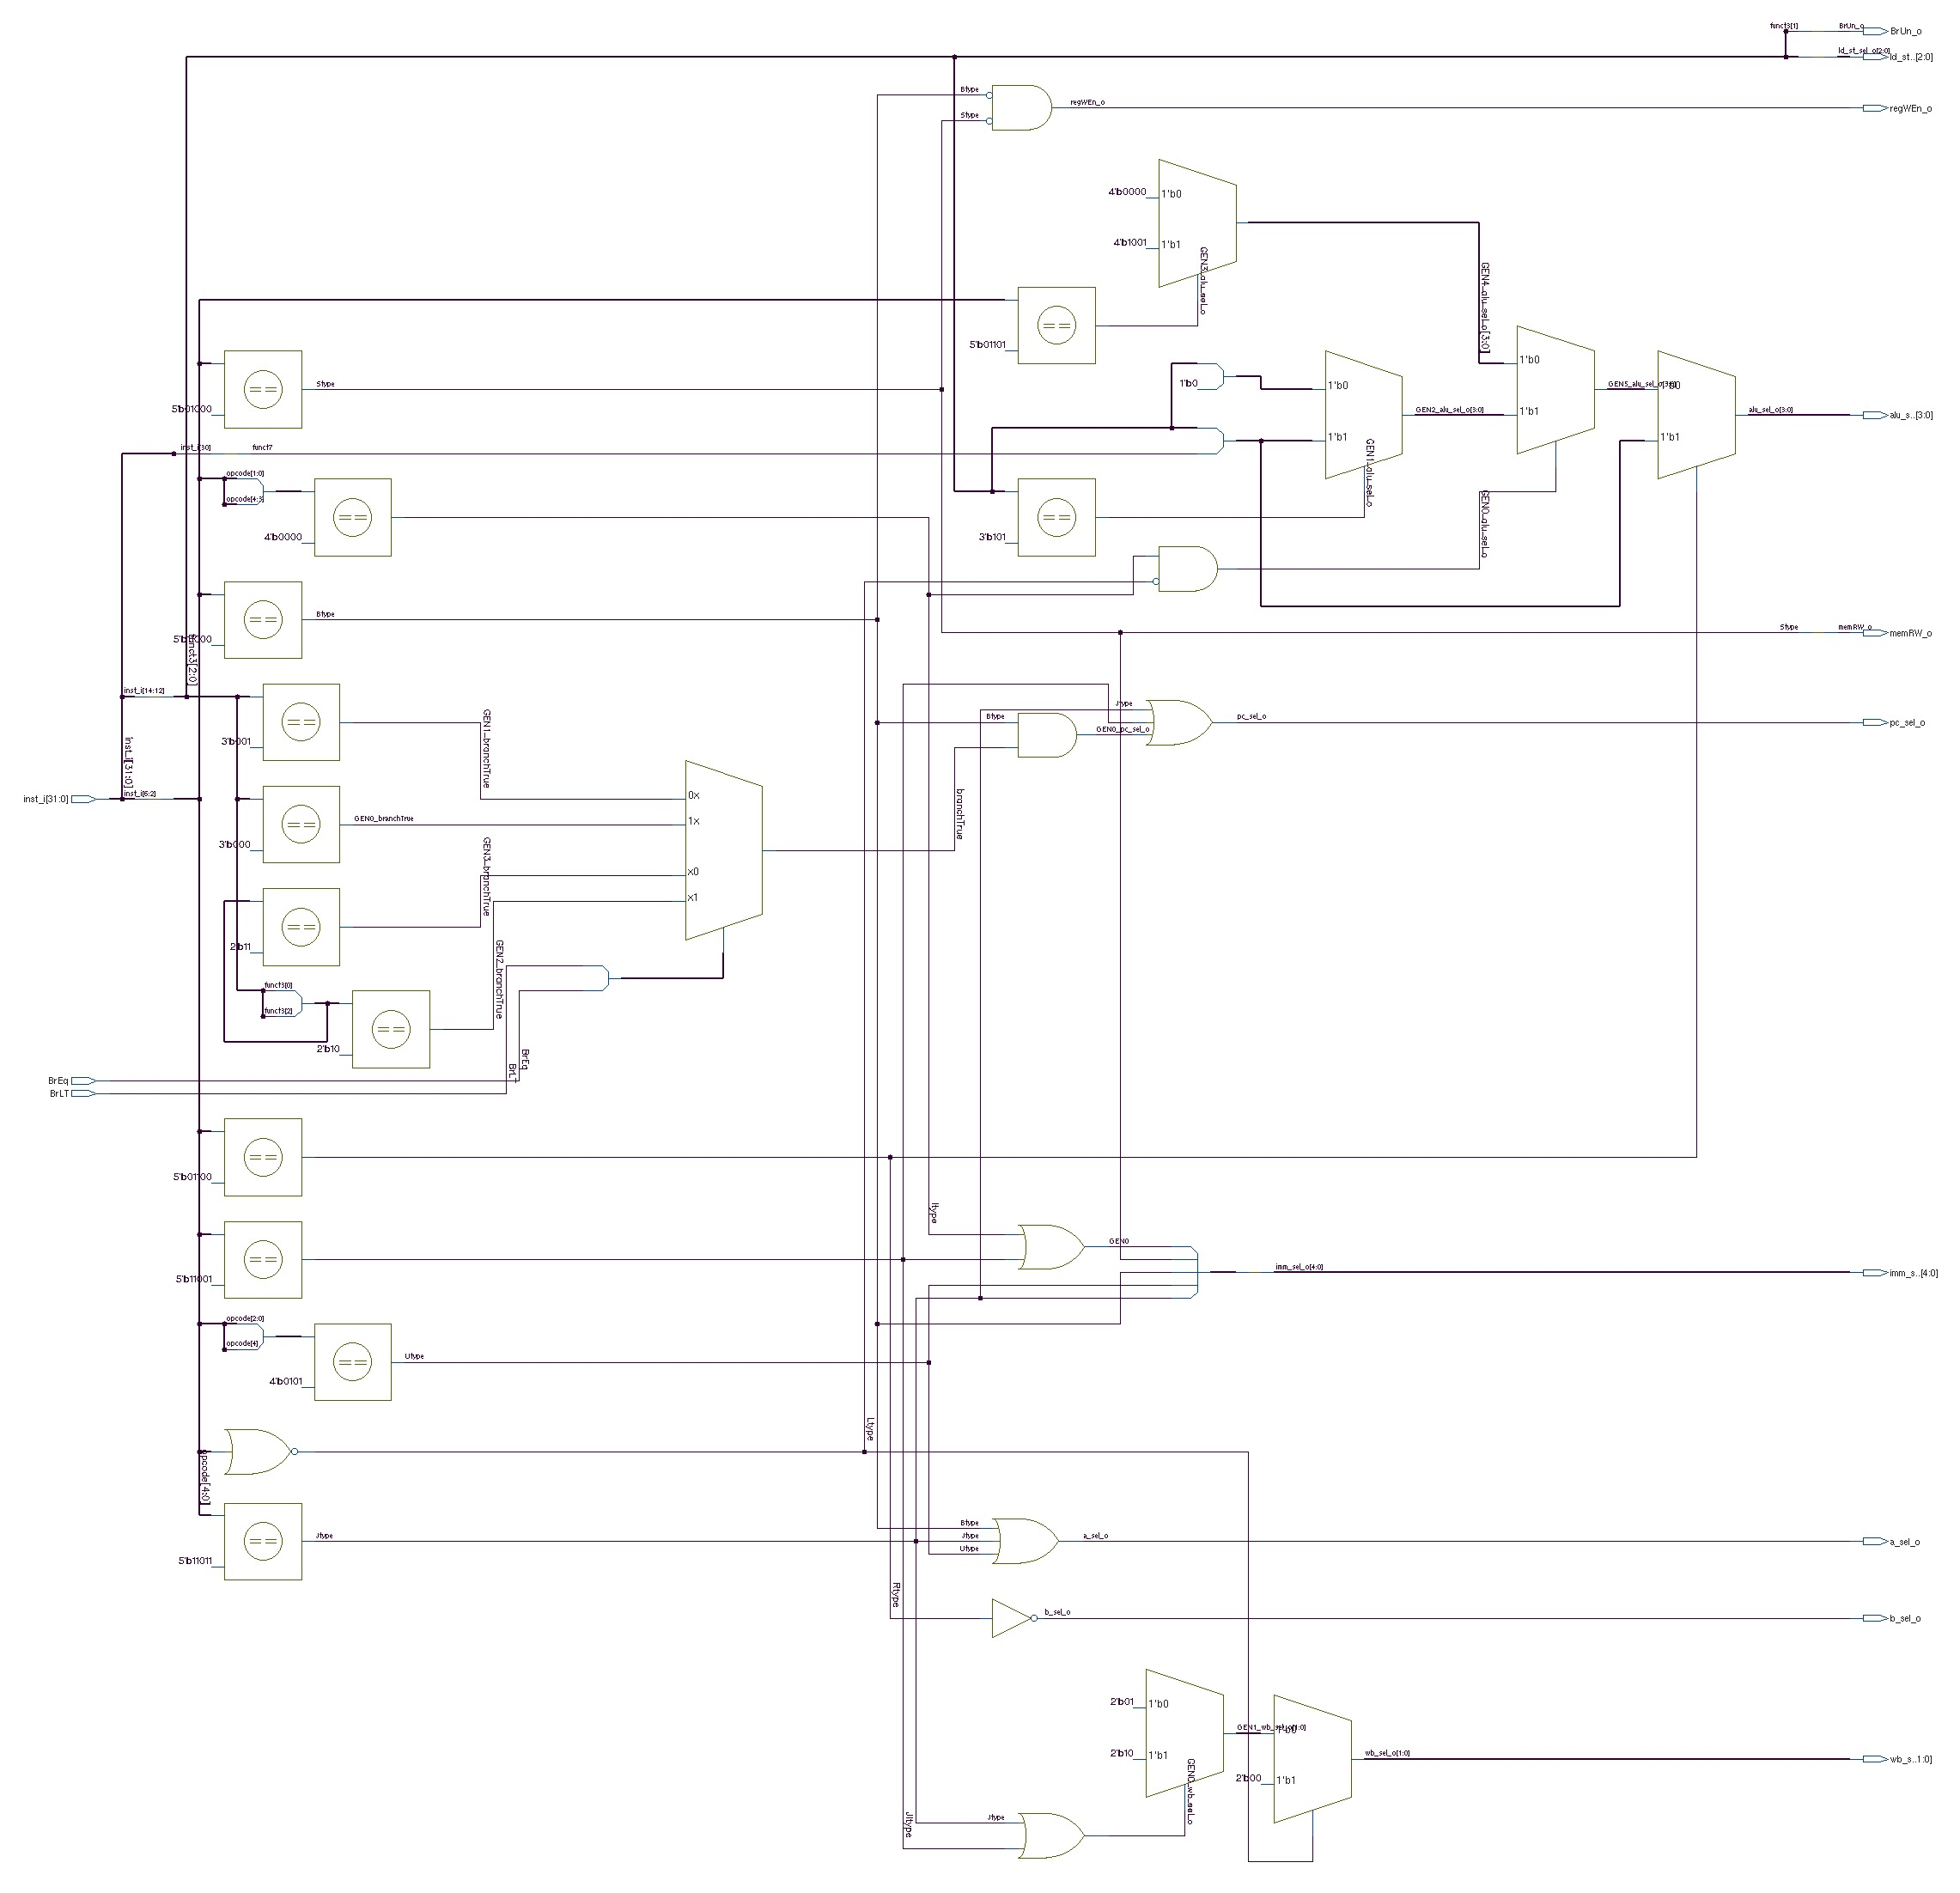
\includegraphics[width=.9\textwidth]{images/ctrl_logic.jpg}
    \caption{Control Unit Schematic\protect\footnotemark}
\end{figure}
\footnotetext{The schematic is generated using Synopsys Verdi.}

\section{Memory Modules}
Unlike the Von Neumann architecture employed in x86 CPUs, which utilizes a single memory for both programs and data, the RISC or ARM CPU follows the Harvard architecture. In this design, memory is split into IMEM (instruction memory) for storing programs and DMEM (data memory) for storing data.

IMEM functions as same as a ROM, handling combinational read-only operations for program data, while DMEM allows for both read and write operations, capable of simultaneous reading and writing.

\begin{figure}[H]
    \centering
    \subfloat[IMEM]{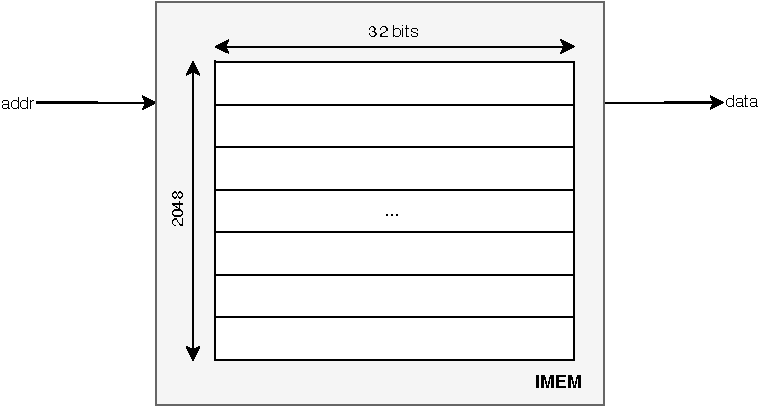
\includegraphics[width=.45\textwidth]{images/imem.pdf}}\subfloat[DMEM]{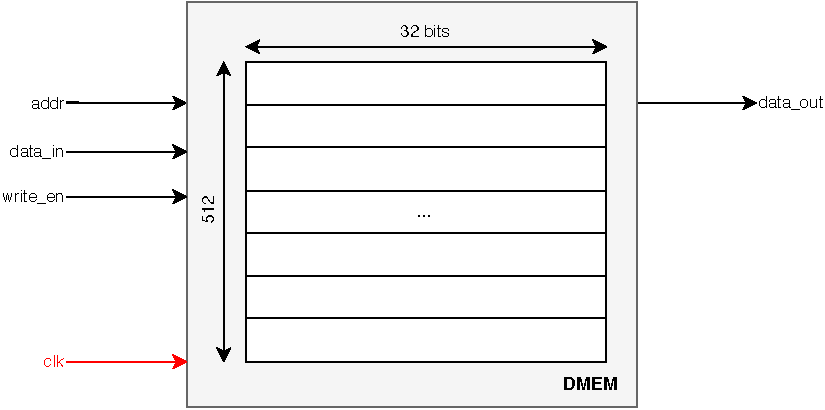
\includegraphics[width=.5\textwidth]{images/dmem.pdf}}
    \caption{Memory modules}
\end{figure}

\section{Load-Store Unit}
A Load-Store Unit (LSU) is a fundamental component of a computer's architecture, specifically within the context of a processor's execution pipeline. It plays a crucial role in modern computer architectures, particularly in processors that follow the Load-Store architecture paradigm, like Reduced Instruction Set Computers (RISC).

The Load-Store Unit is responsible for handling memory-related operations, including loading data from memory, storing data into memory, and performing arithmetic and logical operations on data fetched from memory. 

In this project, the LSU serves as a central component housing a dedicated data memory, alongside a collection of custom-designed elements such as a timer and a binary to Binary-Coded Decimal (BCD) converter. Moreover, the LSU also manages Input/Output (IO) peripherals, including LEDs, 7-segment displays, an LCD1602, keys, switches, and more. Each of these custom components and IO devices is directly accessible through memory-mapped addresses, enabling seamless interaction between the processor and these peripherals. This design facilitates efficient data transfer and control between the processor and the various connected IO devices, offering a well-organized and easily accessible interface for handling input, output, and data manipulation within the system.

Furthermore, the Load-Store Unit (LSU) has been specifically designed to accommodate a range of data transfer operations such as Load Halfword (LH), Load Byte (LB), Load Halfword Unsigned (LHU), Load Byte Unsigned (LBU), Store Halfword (SH), and Store Byte (SB). These operations are integral to accessing and manipulating data stored in memory, enabling the processor to efficiently retrieve specific byte or halfword-sized data and store data back into memory at designated addresses. This comprehensive support for various load and store operations significantly enhances the unit's versatility, allowing for fine-grained control over data transfer and manipulation, ultimately contributing to the system's overall efficiency and flexibility in handling different data types and memory structures.

\begin{figure}[H]
    \centering
    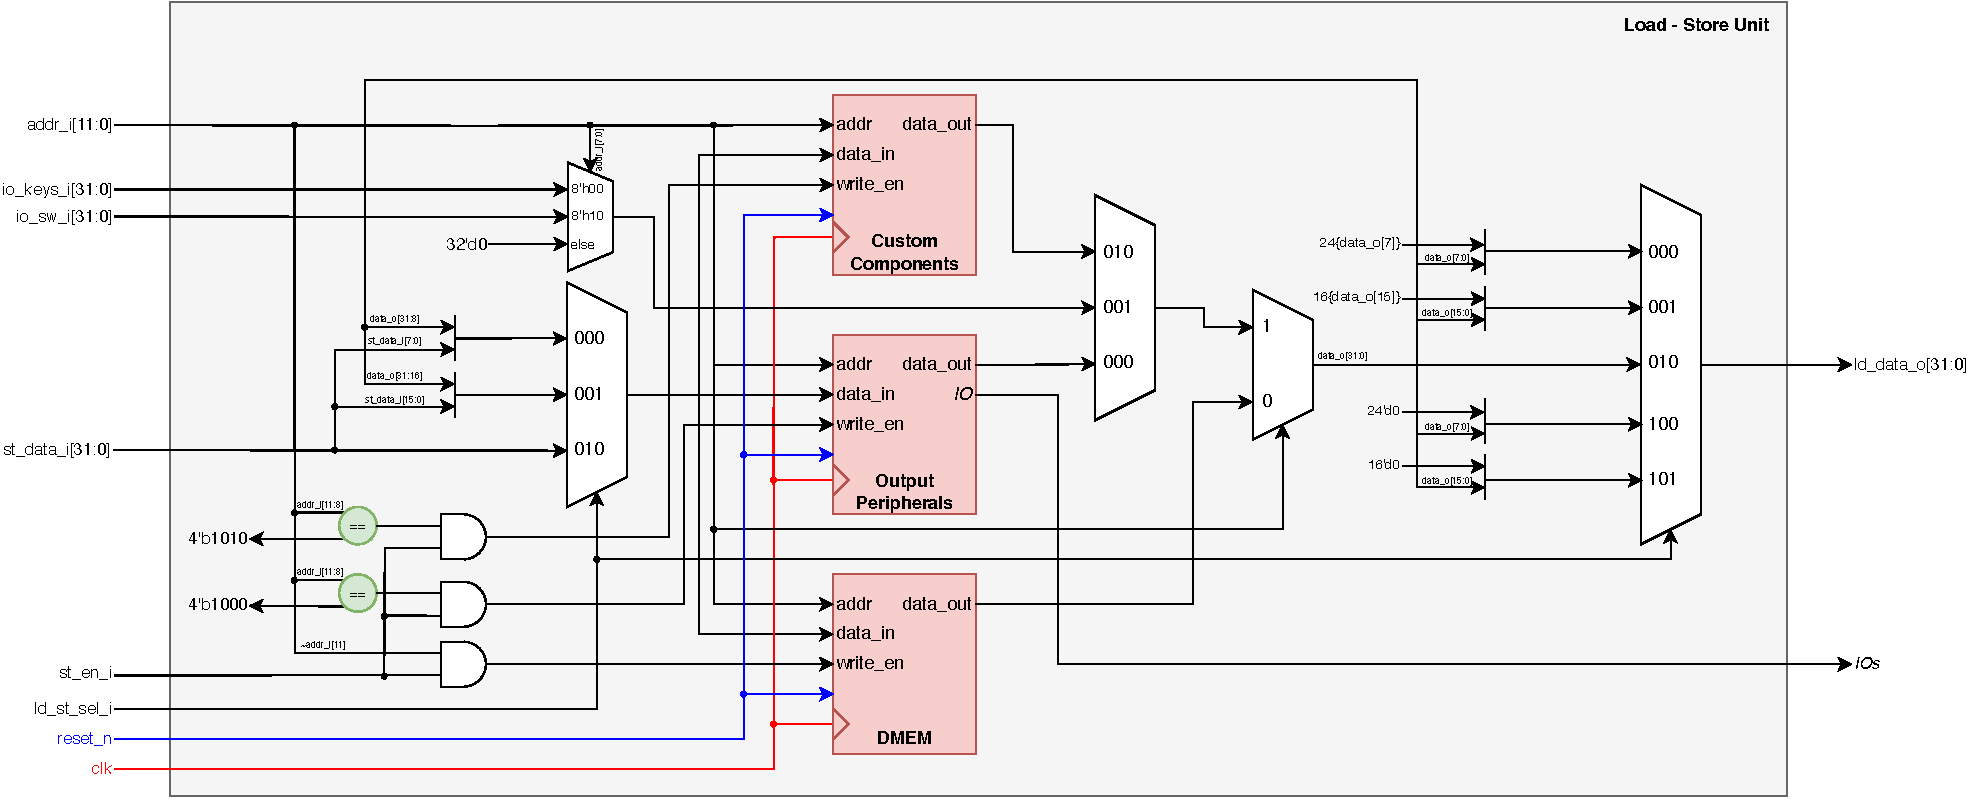
\includegraphics[width=.9\textwidth]{images/lsu.pdf}
    \caption{LSU Block Diagram}
\end{figure}

Below is a visual representation illustrating the memory-mapped addresses associated with all the Input/Output (IO) peripherals and the custom components within the system.

\begin{figure}[H]
    \centering
    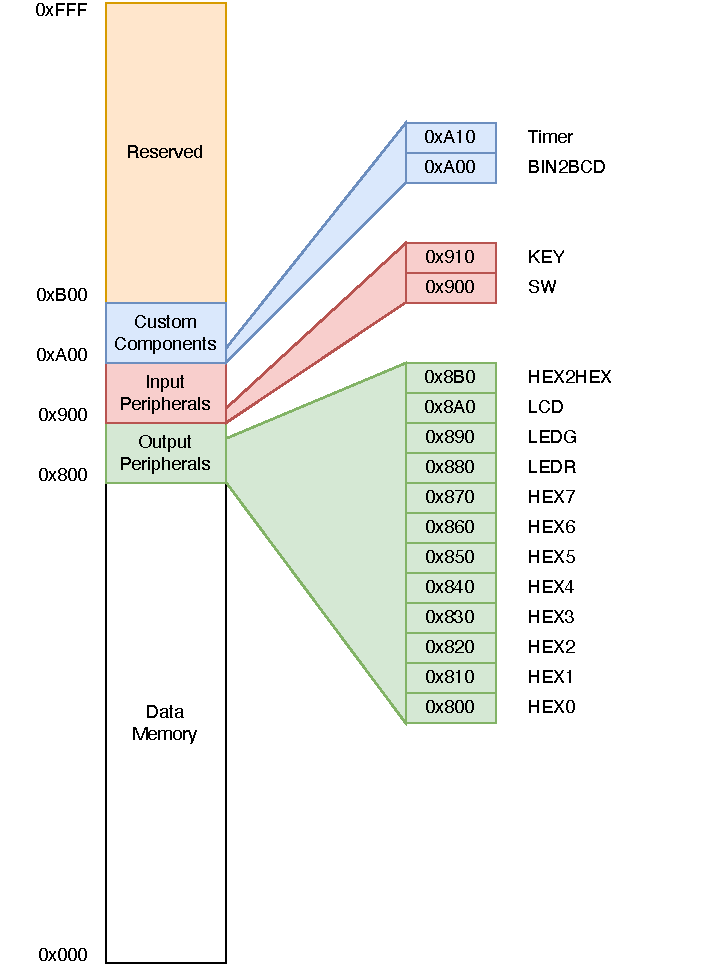
\includegraphics[width=.6\textwidth]{images/memmap.pdf}
    \caption{Memory Mapped Components/IOs}
\end{figure}

\section{Additional Components}
\subsection{Data to 7-segment displays}
The Data to 7-segment displays (HEX2HEX) module is a functional component designed with the capability to perform an automatic conversion process. It takes a 32-bit hexadecimal data as input and efficiently converts each digit within that data into a corresponding set of 7-segment display segments. These individual 7-segment data sets are then directly transmitted and stored on eight separate 7-segment displays. This functionality enables a seamless and accurate presentation of the information contained in the 32-bit hexadecimal data across all eight 7-segment displays without doing the conversions in the software.

The module comprises eight seven-segment control ROM. Each of these ROM units is equipped with 16 memory elements, and each memory address within these ROMs stores a specific value representing the configuration of the seven segments for display.

\begin{figure}[H]
    \centering
    \subfloat[Seven Segment Controller]{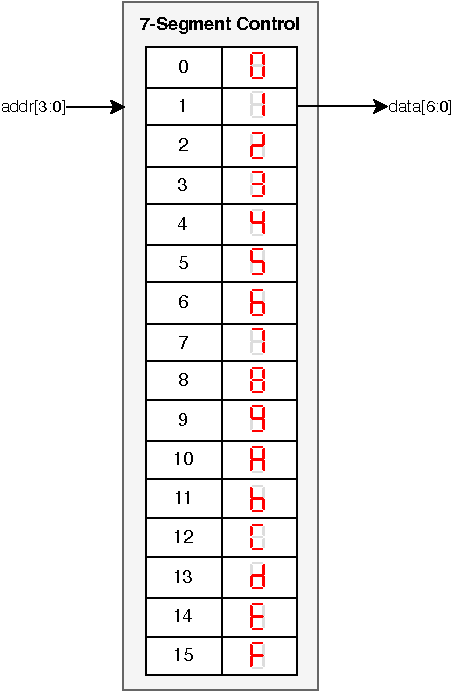
\includegraphics[height=11cm]{images/7segctrl.pdf}}
    \subfloat[Data to 7-segment displays Controller]{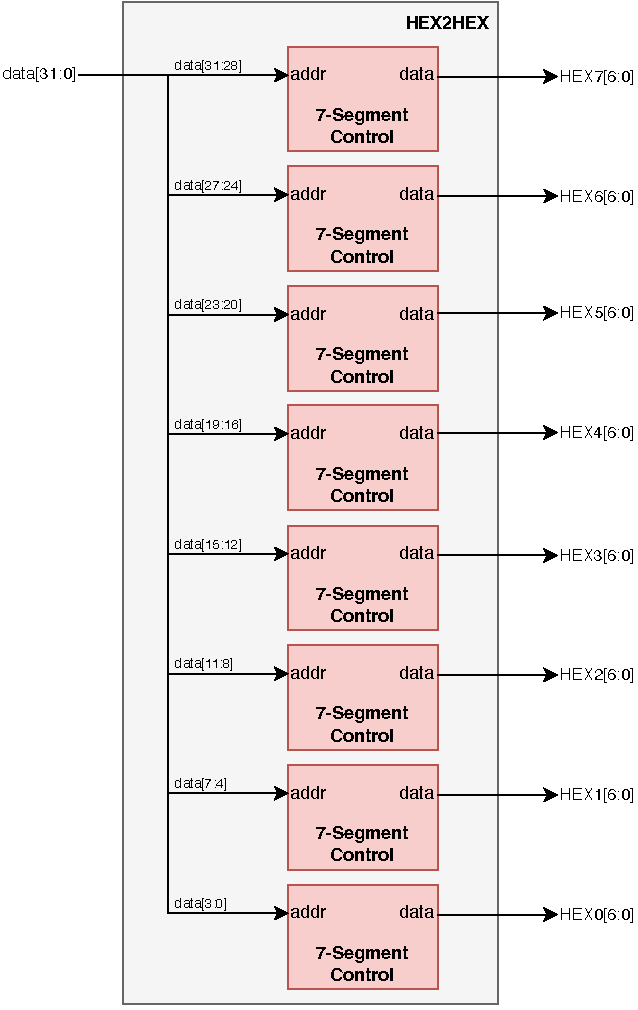
\includegraphics[height=11cm]{images/hex2hex.pdf}}
    \caption{HEX2HEX Block Diagram}
\end{figure}

\subsection{Binary to BCD Converter}

The Binary to Binary-Coded Decimal (BCD) Converter is a module designed to transform numerical data from its binary representation into the BCD format. BCD is a binary-coded decimal system that represents each decimal digit using a 4-bit binary code. This conversion process is essential in various applications, particularly in embedded systems, digital displays, and communication protocols, where human-readable decimal data needs to be processed or displayed.

\subsubsection{Introduction}
The operation of a Binary to BCD Converter typically involves taking binary input, which may be in various binary formats such as 8-bit, 16-bit, or 32-bit, and breaking it down into its individual decimal digits.

For instance, if the binary input is \texttt{00110110}, which is 54 in decimal, the Binary to BCD Converter would transform it into its equivalent BCD representation, which would be \texttt{0101\_0100}, which are the number 5 and 4.

\subsubsection{Double Dabble and the implementation\protect\footnote{This part is referenced from the Wikipedia page on Double Dabble, accessed at \url{https://en.wikipedia.org/wiki/Double\_dabble}.\label{footnote 1}}}

The hardware for this converter utilizes a double dabble algorithm. The double dabble algorithm is a well-known and efficient method for converting binary numbers into BCD format. It's commonly used in digital hardware designs where hardware resources are limited, and an efficient conversion process is necessary.

If the original number to be converted is stored in a register that is $n$ bits wide, a scratch space wide enough to hold both the original number and its BCD representation should be reserved, which will require $n + 4\times \left\lceil\dfrac n3\right\rceil$ bits.

The double dabble algorithm operates by iteratively shifting the binary number leftwards, performing decimal addition to correct any digits that exceed nine in value. This process continues until all digits are within the 0-9 range, and the result is represented in BCD form.

\begin{table}[H]
    \centering
    \begin{tabular}{|ccc|c|l|}
        \hline
        \multicolumn{3}{|c|}{BCD}                                      & \multirow{2}{*}{Binary} & \multicolumn{1}{c|}{\multirow{2}{*}{Comment}} \\ \cline{1-3}
        \multicolumn{1}{|c|}{100's} & \multicolumn{1}{c|}{10's} & 1's  &                         & \multicolumn{1}{c|}{}                       \\ \hline
        \multicolumn{1}{|c|}{\texttt{0000}}  & \multicolumn{1}{c|}{\texttt{0000}} & \texttt{0000} & \texttt{11110011}                & Initialization                              \\ \hline
        \multicolumn{1}{|c|}{\texttt{0000}}  & \multicolumn{1}{c|}{\texttt{0000}} & \texttt{0001} & \texttt{1110011-}                & Shift                                       \\ \hline
        \multicolumn{1}{|c|}{\texttt{0000}}  & \multicolumn{1}{c|}{\texttt{0000}} & \texttt{0011} & \texttt{110011--}                & Shift                                       \\ \hline
        \multicolumn{1}{|c|}{\texttt{0000}}  & \multicolumn{1}{c|}{\texttt{0000}} & \texttt{0111} & \texttt{10011---}                & Shift                                       \\ \hline
        \multicolumn{1}{|c|}{\texttt{0000}}  & \multicolumn{1}{c|}{\texttt{0000}} & \texttt{1010} & \texttt{10011000}                & Add 3 to 1's, since it was 7               \\ \hline
        \multicolumn{1}{|c|}{\texttt{0000}}  & \multicolumn{1}{c|}{\texttt{0001}} & \texttt{0101} & \texttt{0011----}                & Shift                                       \\ \hline
        \multicolumn{1}{|c|}{\texttt{0000}}  & \multicolumn{1}{c|}{\texttt{0001}} & \texttt{1000} & \texttt{0011----}                & Add 3 to 1's, since it was 5               \\ \hline
        \multicolumn{1}{|c|}{\texttt{0000}}  & \multicolumn{1}{c|}{\texttt{0011}} & \texttt{0000} & \texttt{011-----}                & Shift                                       \\ \hline
        \multicolumn{1}{|c|}{\texttt{0000}}  & \multicolumn{1}{c|}{\texttt{0110}} & \texttt{0000} & \texttt{11------}                & Shift                                       \\ \hline
        \multicolumn{1}{|c|}{\texttt{0000}}  & \multicolumn{1}{c|}{\texttt{1001}} & \texttt{0000} & \texttt{11------}                & Add 3 to 10's, since it was 6               \\ \hline
        \multicolumn{1}{|c|}{\texttt{0001}}  & \multicolumn{1}{c|}{\texttt{0010}} & \texttt{0001} & \texttt{1-------}                & Shift                                       \\ \hline
        \multicolumn{1}{|c|}{\texttt{0010}}  & \multicolumn{1}{c|}{\texttt{0100}} & \texttt{0011} & \texttt{--------}                & Shift                                       \\ \hline
        \multicolumn{1}{|c|}{2}     & \multicolumn{1}{c|}{4}    & 3    & ~                       & ~                                           \\ \hline
    \end{tabular}
\end{table}

The diagram for the Binary to BCD Hardware Implementation has been proposed by Ameer Abdelhadi\textsuperscript{\ref{footnote 1}}. In this project, we will incorporate and allocate it to the memory address \texttt{0xA00} for the input and \texttt{0xA04} for the output.

\begin{figure}[H]
    \centering
    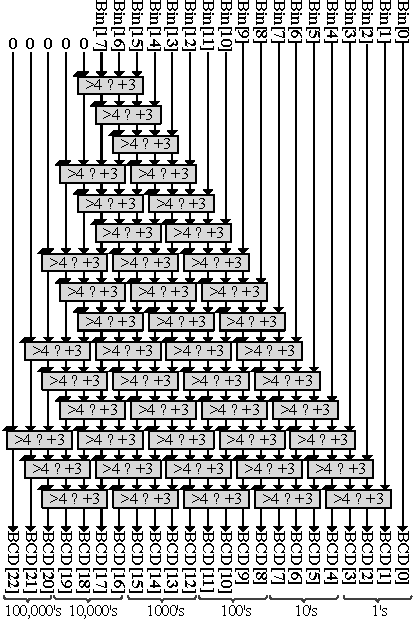
\includegraphics[width=.8\textwidth]{images/bin2bcd.pdf}
    \caption{Binary to BCD Hardware Implementation}
\end{figure}

\begin{figure}[H]
    \centering
    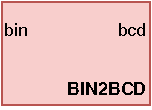
\includegraphics[width=.3\textwidth]{images/bin2bcd_symbol.pdf}
    \caption{Binary to BCD Symbol}
\end{figure}

\subsection{Timer}
The timer is a fundamental component within a Central Processing Unit (CPU) that plays a pivotal role in computer systems. It is responsible for tracking and managing the passage of time, serving as a critical element for various system operations. The timer can be used for a multitude of purposes, including scheduling tasks, measuring execution time, and enabling real-time operations. It often operates at a high precision, allowing for the accurate measurement of intervals and the synchronization of tasks. In the context of CPU operations, the timer provides essential timing and control signals to coordinate the execution of instructions, ensuring the efficient and orderly processing of data and tasks. Additionally, it finds applications in performance monitoring, power management, and system events, making it an indispensable part of modern CPU architectures.

\subsubsection{Timer parameters}
The initial timer value and the prescaler are key parameters that influence the operation and precision of a timer within a CPU. The initial timer value, often referred to as the ``timer start value'' or ``count'', determines where the timer begins counting from when it is activated. This value can be set to any desired starting point, allowing for flexibility in timing applications. The choice of the initial timer value depends on the specific use case and the desired timing requirements.

The prescaler, on the other hand, is a configurable component that divides the input clock frequency before it reaches the timer. It allows for the adjustment of the timer's granularity, effectively extending the range and precision of the timer. By dividing the clock frequency, the prescaler can make the timer count at a slower rate, which can be especially useful when the timer needs to measure longer time intervals or when a finer level of precision is required.

Let's consider an example in the context of an embedded system with a microcontroller. Suppose the initial timer value is set to 390625 and a prescaler is configured to divide the clock signal by 128. In this scenario, the timer would start counting down from 390625, and each count would represent 128 clock cycles. This effectively extends the timer's range and precision. If the clock signal has a frequency of 50 MHz, the timer would generate an interrupt or trigger an event when $128\times 390625$ clock cycles have occurred, which corresponds to $\dfrac{128\times 390625}{50,000,000} = $ 1 second. This combination of the initial timer value and the prescaler allows for versatile timing capabilities in various applications, from controlling the execution of tasks to measuring time intervals with precision.

\begin{figure}[H]
    \centering
    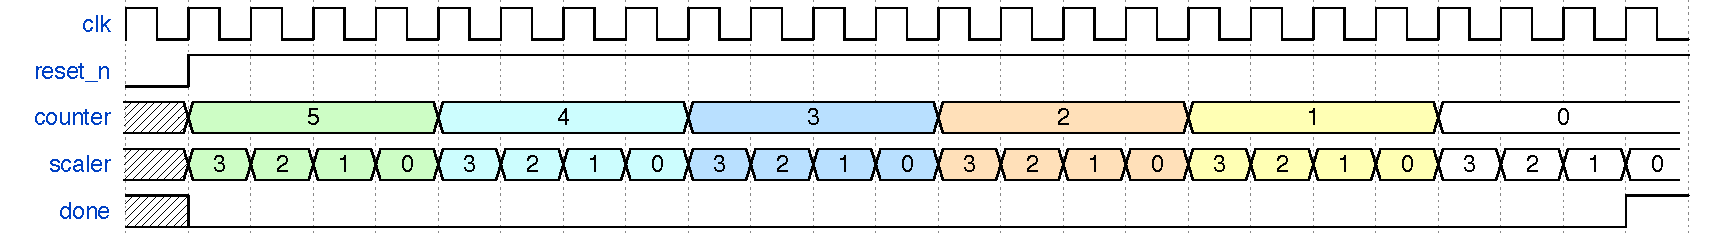
\includegraphics[width=\textwidth]{images/timer_wave.pdf}
    \caption{Timer with prescaler = 4, initial value = 5}
\end{figure}

\subsubsection{Timer Hardware Design}
In the presented design, the system takes three inputs: \texttt{init\_value}, \texttt{prescaler}, and \texttt{enable}. Notably, the effective prescaler value is determined by $2^{\texttt{prescaler}}$. Upon a reset, the initial value is loaded into the counter register, and the scaler register is reset to zero. When the \texttt{enable} signal is activated, the scaler begins accumulating. As the scaler count approaches the specified prescaler value, the counter value is decremented. This process continues until both the scaler and counter reach zero, at which point the \texttt{done} signal is asserted. The timer can be reactivated by utilizing the \texttt{reset} signal.

\begin{figure}[H]
    \centering
    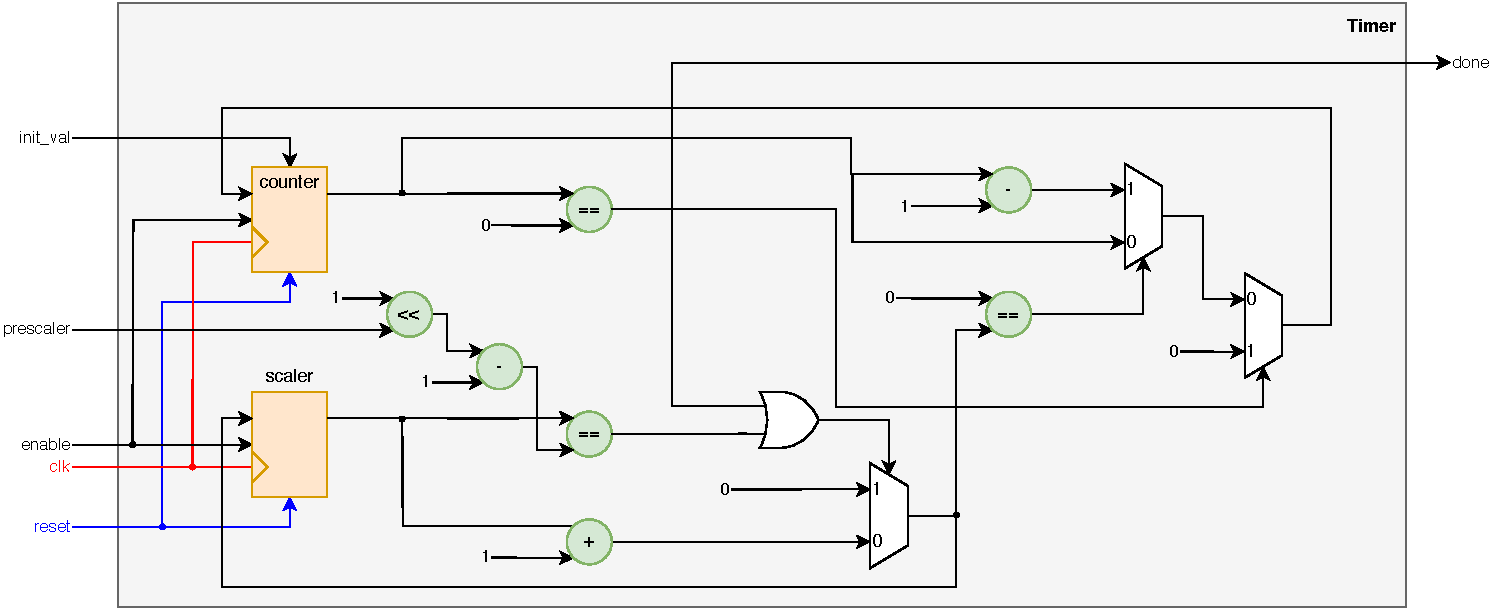
\includegraphics[width=.95\textwidth]{images/timer.pdf}
    \caption{Timer Block Diagram}
\end{figure}

To facilitate seamless communication with our CPU, we have developed a Timer Wrapper module. This module takes input data in a specified format, as illustrated in the provided table. The timer will be allocated at the memory address from \texttt{0xA10} to \texttt{0xA1C}.

\begin{table}[H]
\centering
\caption{Read/Write data address for Timer}
\begin{tabular}{|l|c|ll|l|}
\hline
\multirow{2}{*}{RW}    & \multirow{2}{*}{Address} & \multicolumn{2}{c|}{Data bits}                     & \multicolumn{1}{c|}{\multirow{2}{*}{Description}}                                       \\ \cline{3-4}
                       &                          & \multicolumn{1}{c|}{31:1} & \multicolumn{1}{c|}{0} & \multicolumn{1}{c|}{}                                                                   \\ \hline
\multirow{3}{*}{Write} & \texttt{0xA10}                    & \multicolumn{2}{l|}{Initial Value}                 & Set the initial value                                                                   \\ \cline{2-5} 
                       & \texttt{0xA14}                    & \multicolumn{2}{l|}{Prescaler}                     & Set the prescaler                                                                       \\ \cline{2-5} 
                       & \texttt{0xA18}                    & \multicolumn{1}{l|}{x}    & 0/1                    & \begin{tabular}[c]{@{}l@{}}0: Reset and enable timer\\ 1: Enable the timer\end{tabular} \\ \hline
Read                   & \texttt{0xA1C}                    & \multicolumn{1}{l|}{x}    & done                   & Done signal of the timer                                                                \\ \hline
\end{tabular}
\end{table}

\begin{figure}[H]
    \centering
    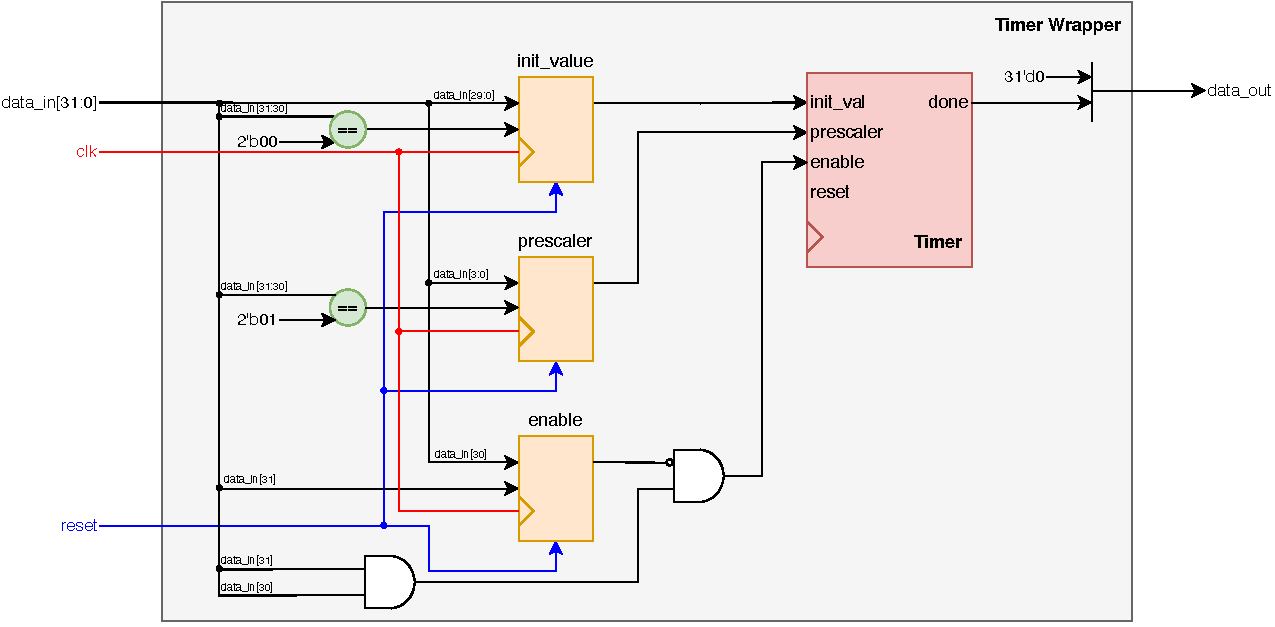
\includegraphics[width=.9\textwidth]{images/timer_wrapper.pdf}
    \caption{Timer Wrapper Block Diagram}
\end{figure}


\chapter{Verification Strategy}
\section{ALU}
The ALU testbench plays role in validating the ALU module's functionality. It achieves this by subjecting the module to a series of tests based on the \texttt{sel} signal, as outlined in Table \ref{alu}. This thorough testing ensures that the ALU can perform various operations accurately.

During the testing process, the testbench generates random binary inputs, converts them into their hexadecimal equivalents, and then compares the module's output to the expected hexadecimal values, derived from the input. This testing process is repeated for a specified number of simulation cycles, with each test being marked as a pass or fail. In the results provided, all 15 test inputs have passed, confirming that the ALU module is performing as expected for the given test cases.
\begin{minted}{text}
inA         inB             sel     output          expected output
f1ffebb     4882e226        0       57a2e0e1        57a2e0e1
f1ffebb     4882e226        1       c7ffaec0        c7ffaec0
f1ffebb     4882e226        2       1               1
f1ffebb     4882e226        3       1               1
f1ffebb     4882e226        4       479d1c9d        479d1c9d
f1ffebb     4882e226        5       3c7ffa          3c7ffa
f1ffebb     4882e226        6       4f9ffebf        4f9ffebf
f1ffebb     4882e226        7       802e222         802e222
f1ffebb     4882e226        8       c69d1c95        c69d1c95
f1ffebb     4882e226        9       4882e226        4882e226
f1ffebb     4882e226        a       0               0
f1ffebb     4882e226        b       0               0
f1ffebb     4882e226        c       0               0
f1ffebb     4882e226        d       3c7ffa          3c7ffa
f1ffebb     4882e226        e       0               0
f1ffebb     4882e226        f       0               0
All tests passed!
\end{minted}
\section{Branch Comparator}
The testing approach for the hardware module \textbf{Branch Comparator} involves implementing it with assertion writing in SystemVerilog and subjecting it to a rigorous testbench with \texttt{500} randomized test cases, generated using the \texttt{\$urandom} macro function. To ensure the occurrence of equality scenarios, a condition is incorporated to generate equal inputs for the DUT module every ten times. Testing the software comparison of two inputs in the testbench is somewhat intricate due to the need to handle two types of variables: \texttt{int unsigned r1u, r2u;} and \texttt{int signed r1s, r2s;} to yield the correct boolean output when \texttt{br\_unsigned} is randomized, indicating whether the hardware module should compare signed or unsigned 32-bit numbers. The key verification mechanism is the assertion, immediately evaluating whether the output of the software testbench matches the output flag of the hardware DUT. This assertion is invoked whenever there is a change in the generated inputs, resulting in the generation of 500 messages for each true or false assertion outcome.
\begin{minted}{text}
<PASS>   0: rs1 = 12153524, rs2 = 00000000, BrUn = 0, BrLT = 0, BrEq = 0
<PASS>   1: rs1 = c0895e81, rs2 = 8484d609, BrUn = 0, BrLT = 0, BrEq = 0
<PASS>   2: rs1 = b1f05663, rs2 = 06b97b0d, BrUn = 0, BrLT = 1, BrEq = 0
<PASS>   3: rs1 = 46df998d, rs2 = b2c28465, BrUn = 0, BrLT = 0, BrEq = 0
<PASS>   4: rs1 = 89375212, rs2 = 00f3e301, BrUn = 0, BrLT = 1, BrEq = 0
<PASS>   5: rs1 = 06d7cd0d, rs2 = 3b23f176, BrUn = 0, BrLT = 1, BrEq = 0
<PASS>   6: rs1 = 1e8dcd3d, rs2 = 76d457ed, BrUn = 0, BrLT = 1, BrEq = 0
<PASS>   7: rs1 = 462df78c, rs2 = 7cfde9f9, BrUn = 0, BrLT = 1, BrEq = 0
<PASS>   8: rs1 = 3386553a, rs2 = 46f91c6a, BrUn = 1, BrLT = 1, BrEq = 0
<PASS>   9: rs1 = e33724c6, rs2 = e2f784c5, BrUn = 0, BrLT = 0, BrEq = 0
<PASS>  10: rs1 = e33724c6, rs2 = e33724c6, BrUn = 1, BrLT = 0, BrEq = 1
........................................................................
<PASS> 490: rs1 = 62fd49c5, rs2 = 49a84ac9, BrUn = 0, BrLT = 0, BrEq = 0
<PASS> 491: rs1 = 67d735cf, rs2 = 4839e590, BrUn = 0, BrLT = 0, BrEq = 0
<PASS> 492: rs1 = a8e4d851, rs2 = b4f9a469, BrUn = 0, BrLT = 1, BrEq = 0
<PASS> 493: rs1 = 3b83cd77, rs2 = 2523654a, BrUn = 0, BrLT = 0, BrEq = 0
<PASS> 494: rs1 = ec3758d8, rs2 = 4ddd4d9b, BrUn = 0, BrLT = 1, BrEq = 0
<PASS> 495: rs1 = 150b24aa, rs2 = 204cc13d, BrUn = 1, BrLT = 1, BrEq = 0
<PASS> 496: rs1 = e20e9ac4, rs2 = 5c78b1b8, BrUn = 0, BrLT = 1, BrEq = 0
<PASS> 497: rs1 = dbe6f2b7, rs2 = c378ee86, BrUn = 0, BrLT = 0, BrEq = 0
<PASS> 498: rs1 = 32a71548, rs2 = f5fbe062, BrUn = 1, BrLT = 1, BrEq = 0
<PASS> 499: rs1 = 5094c2d3, rs2 = 9fd823fc, BrUn = 1, BrLT = 1, BrEq = 0
\end{minted}


\section{Immediate Generator}
Similar to the \textbf{Branch Comparator}, we apply a rigorous testing methodology to the \textbf{Immediate Generator} hardware module, subjecting it to 500 test cases. However, there's a notable distinction in the output generation between the SystemVerilog (SV) hardware implementation and the SV software testbench. While both generate immediates using bit-concatenation, the hardware utilizes a straightforward ternary conditional expression, \texttt{[condition]?[assignment\_true]:[assignment\_false]}, effectively acting as a basic selection multiplexer. This approach enhances the trustworthiness and precision of the module's verification process. The instruction, serving as the input for both the Design Under Test (DUT) and the software testbench, is randomized using the \texttt{\$random} SV function. The selection signal undergoes similar randomization. To validate the module's correctness, the testbench employs immediate assertions, comparing the software output against the DUT's output. Any assertion failure results in a testbench failure, ensuring a robust verification process.
\begin{minted}{text}
<PASS> 0: ImmSel = 00000 Imm = 00000000 , Instruction = edeacadc
<PASS> 1: ImmSel = 00000 Imm = 00000000 , Instruction = 8484d609
<PASS> 2: ImmSel = 00100 Imm = 00000076 , Instruction = 06b97b0d
<PASS> 3: ImmSel = 00000 Imm = 00000000 , Instruction = b2c28465
<PASS> 4: ImmSel = 10000 Imm = 0003e80e , Instruction = 00f3e301
<PASS> 5: ImmSel = 00100 Imm = 000003a2 , Instruction = 3b23f176
<PASS> 6: ImmSel = 00100 Imm = 00000f6e , Instruction = 76d457ed
<PASS> 7: ImmSel = 00001 Imm = fffff830 , Instruction = 83021607
<PASS> 8: ImmSel = 00000 Imm = 00000000 , Instruction = e2f784c5
<PASS> 9: ImmSel = 00000 Imm = 00000000 , Instruction = 72aff7e5
<PASS> 10: ImmSel = 10000 Imm = fff2d892 , Instruction = 8932d612
..................................................................
<PASS> 490: ImmSel = 01000 Imm = 384bc000 , Instruction = 384bc571
<PASS> 491: ImmSel = 00000 Imm = 00000000 , Instruction = 3da8cd7b
<PASS> 492: ImmSel = 00000 Imm = 00000000 , Instruction = b7f4306f
<PASS> 493: ImmSel = 00100 Imm = fffffe40 , Instruction = e4d820c9
<PASS> 494: ImmSel = 00000 Imm = 00000000 , Instruction = 6d48a5da
<PASS> 495: ImmSel = 00100 Imm = 00000ee2 , Instruction = 6fcff1df
<PASS> 496: ImmSel = 01000 Imm = 384d4000 , Instruction = 384d4170
<PASS> 497: ImmSel = 10000 Imm = 00093d72 , Instruction = 57393baf
<PASS> 498: ImmSel = 00000 Imm = 00000000 , Instruction = f612c8ec
<PASS> 499: ImmSel = 10000 Imm = 000bbffc , Instruction = 7fdbb3ff
\end{minted}
\section{Control Unit}
A testbench is designed to verify the functionality of a control unit by applying a series of test cases. It instantiates the \texttt{control\_logic} modules, assigns inputs based on defined test cases, and compares the outputs to expected values. The testbench simulates different instructions represented by binary codes and verifies the output against the expected results using ``don't care'' placeholders to allow partial matches. The testbench loops through 2048 ($2^{11}$) test cases, evaluating and counting the number of passed cases to determine the success rate of the module's behavior, finally concluding the simulation and displaying the success rate.

The list of test cases in the Verilog testbench is generated based on the instruction format and encoding defined in table \ref{ctrl_unit}.

\begin{minted}{text}
LB: PASSED
ADDI: PASSED
AUIPC: PASSED
SB: PASSED
ADD: PASSED
LUI: PASSED
BEQ: PASSED
JALR: PASSED
JAL: PASSED
LH: PASSED
SLLI: PASSED
...
AUIPC: PASSED
LUI: PASSED
BLTU: PASSED
JALR: PASSED
JAL: PASSED
ANDI: PASSED
AUIPC: PASSED
LUI: PASSED
JALR: PASSED
JAL: PASSED
Pass rate:        2048/       2048
\end{minted}


\section{Load -- Store Unit}
The LSU (Load-Store Unit) testbench is divided into three distinct parts: DMEM (Data Memory) test, input peripheral test, and output peripheral test. In the DMEM test, 10240 random data values are stored at 10240 random addresses. Following the write operation, an immediate read is performed at each address, and the test checks whether the randomly written data matches the read data.

For the input peripheral test, random data is set to both switches (SWs) and keys (KEYs). Subsequently, a read operation is executed, and the test verifies whether the data from both SWs and KEYs corresponds to the read data. Lastly, in the output peripheral test, random data is stored in the output peripherals. The test then checks whether the output data matches the initially written data. Both the input and output peripheral tests are repeated for 100 passes.

\begin{minted}{text}
===== DMEM test =====
0x524: stored c0895e81
0x524:   read c0895e81 => Matched
0x609: stored b1f05663
0x609:   read b1f05663 => Matched
0x30d: stored 46df998d
0x30d:   read 46df998d => Matched
0x465: stored 89375212
0x465:   read 89375212 => Matched
0x301: stored 06d7cd0d
0x301:   read 06d7cd0d => Matched
0x176: stored 1e8dcd3d
0x176:   read 1e8dcd3d => Matched
0x7ed: stored 462df78c
0x7ed:   read 462df78c => Matched
0x1f9: stored e33724c6
0x1f9:   read e33724c6 => Matched
0x4c5: stored d513d2aa
0x4c5:   read d513d2aa => Matched
0x7e5: stored bbd27277
0x7e5:   read bbd27277 => Matched
0x612: stored 47ecdb8f
0x612:   read 47ecdb8f => Matched
0x1f2: stored e77696ce
0x1f2:   read e77696ce => Matched
// 10240 times

===== IO test =====
** PASS           0 **
===> Input peripherals test
SW:           1ccb3139
0x900:   read 1ccb3139 => Matched
KEYS:         8e102a1c
0x910:   read 8e102a1c => Matched
===> Output peripherals test
[HEXes]
0x800: stored bdd2327b
Read data: bdd2327b => Matched.
0x810: stored de8f02bd
Read data: de8f02bd => Matched.
0x820: stored 7c8537f9
Read data: 7c8537f9 => Matched.
0x830: stored af91245f
Read data: af91245f => Matched.
0x840: stored 190ba132
Read data: 190ba132 => Matched.
0x850: stored 442ebf88
Read data: 442ebf88 => Matched.
0x860: stored b5915e6b
Read data: b5915e6b => Matched.
0x870: stored 24401948
Read data: 24401948 => Matched.
[LEDR]
0x880: stored 5f84cdbf
Read data: 5f84cdbf => Matched.
[LEDG]
0x890: stored 0749f90e
Read data: 0749f90e => Matched.
[LCD]
0x8a0: stored 8fbf921f
Read data: 8fbf921f => Matched.
// 100 times
\end{minted}

\section{Additional Components}
\subsection{Binary to BCD Converter}
A testbench initializes a parameter for the maximum simulation cycles, sets up input and output signals, and defines a function \texttt{check\_bcd} to verify the correctness of the BCD conversion. The testbench generates random binary input values, converts them to BCD using the \texttt{bin2bcd} module, and compares the module's output to an expected BCD representation derived from the input. It repeats this process for a specified number of simulation cycles and reports whether each conversion test passed or failed. Finally, it prints a summary indicating if all tests have passed and terminates the simulation.

Below are the simulation results for only 10 test inputs, all of which passed successfully. Please note that this is just an example with a limited number of inputs for illustration. In our extensive testing, we have verified the functionality using 10,000 inputs multiple times, and all tests passed without any issues.

\begin{minted}{text}
Test 0 - Input:  303379748, Output: 0303379748 => Passed
Test 1 - Input: 3230228097, Output: 3230228097 => Passed
Test 2 - Input: 2223298057, Output: 2223298057 => Passed
Test 3 - Input: 2985317987, Output: 2985317987 => Passed
Test 4 - Input:  112818957, Output: 0112818957 => Passed
Test 5 - Input: 1189058957, Output: 1189058957 => Passed
Test 6 - Input: 2999092325, Output: 2999092325 => Passed
Test 7 - Input: 2302104082, Output: 2302104082 => Passed
Test 8 - Input:   15983361, Output: 0015983361 => Passed
Test 9 - Input:  114806029, Output: 0114806029 => Passed
All Passed.
\end{minted}

\subsection{Timer}
A timer testbench instantiates a \texttt{timer\_wrapper} module, generates a clock signal, and includes a task called \texttt{start\_timer} to test the timer's functionality. The \texttt{start\_timer} task configures the timer with initial values and a prescaler, measures the time it takes for the timer to complete a certain number of cycles, and then checks if the timer's behavior matches the expected outcome. Multiple test cases are executed in the process, where the timer is tested with different initial values and prescaler settings. The testbench evaluates the timer's performance and displays the results as either "Test Passed!" or "Test Failed!" based on the specified criteria.

\begin{minted}{text}
Initial Value: 250, Prescaler: 2
Start time: 60, End time: 10060 => Cycles: 1000
Test Passed!

Initial Value: 500, Prescaler: 4
Start time: 10110, End time: 90110 => Cycles: 8000
Test Passed!
\end{minted}

\begin{figure}[H]
    \hspace{-2cm}
    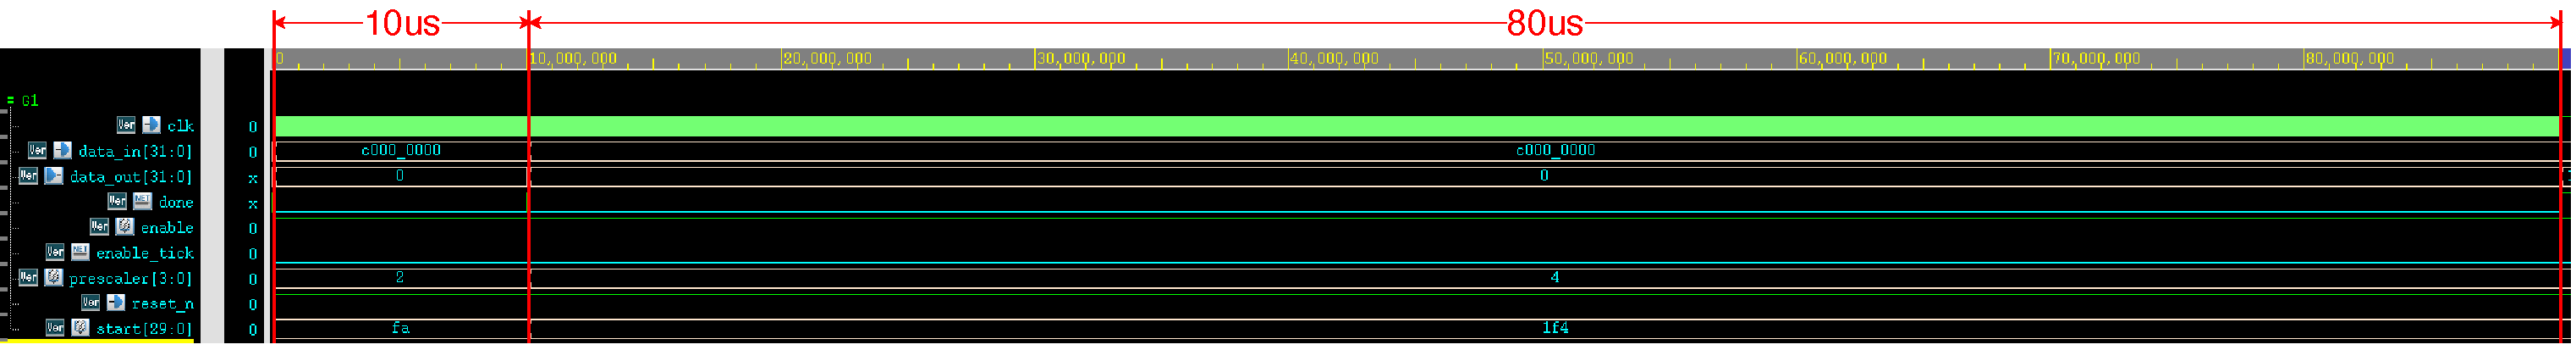
\includegraphics[width=1.2\textwidth]{images/timer_sim_wave.pdf}
    \caption{Timer testbench waveform}
\end{figure}

The given clock cycle duration is \SI{10}{\nano\second}. If we have 1000 cycles, it indeed corresponds to \SI{10,000}{\nano\second}, which is equivalent to \SI{10}{\micro\second}. Similarly, for 8000 cycles, it would amount to \SI{80}{\micro\second}. Therefore, the waveform provided accurately reflects the expected timing results.

\section{Instructions Verification}
To design an effective verification testbench for our RISCV CPU, we should begin by creating a robust assembly implementation tailored to the CPU's specifications. The assembly code can be categorized into two primary segments: one comprising branch and jump instructions, and the other encompassing ALU, Load, and Store instructions. For the sake of simplicity, we'll initiate our efforts with the branch and jump instructions, delineated by eight distinct green address labels, strategically arranged for the instructions \texttt{beq, bne, blt, bltu, bgt, bgtu, jal, and jalr}. As for the ALU, Load, and Store instructions, they will be integrated into the routine associated with the \texttt{jal} jump instruction, while \texttt{auipc and lui} will be assessed within the \texttt{jalr} routine. It's worth emphasizing that, in our quest for efficiency, we have devised specific routines for handling CPU peripheral outputs. In the context of the \texttt{jal} routine, instead of employing the \texttt{ret} syntax (due to its inclusion of peripheral output sub-routines), we opt for the usage of \texttt{la x10, back2main} and \texttt{jalr x10} as a means to seamlessly return to the main program after executing the ALU/Load/Store instructions, streamlining our verification process.

 \begin{figure}[H]
    \begin{center}
    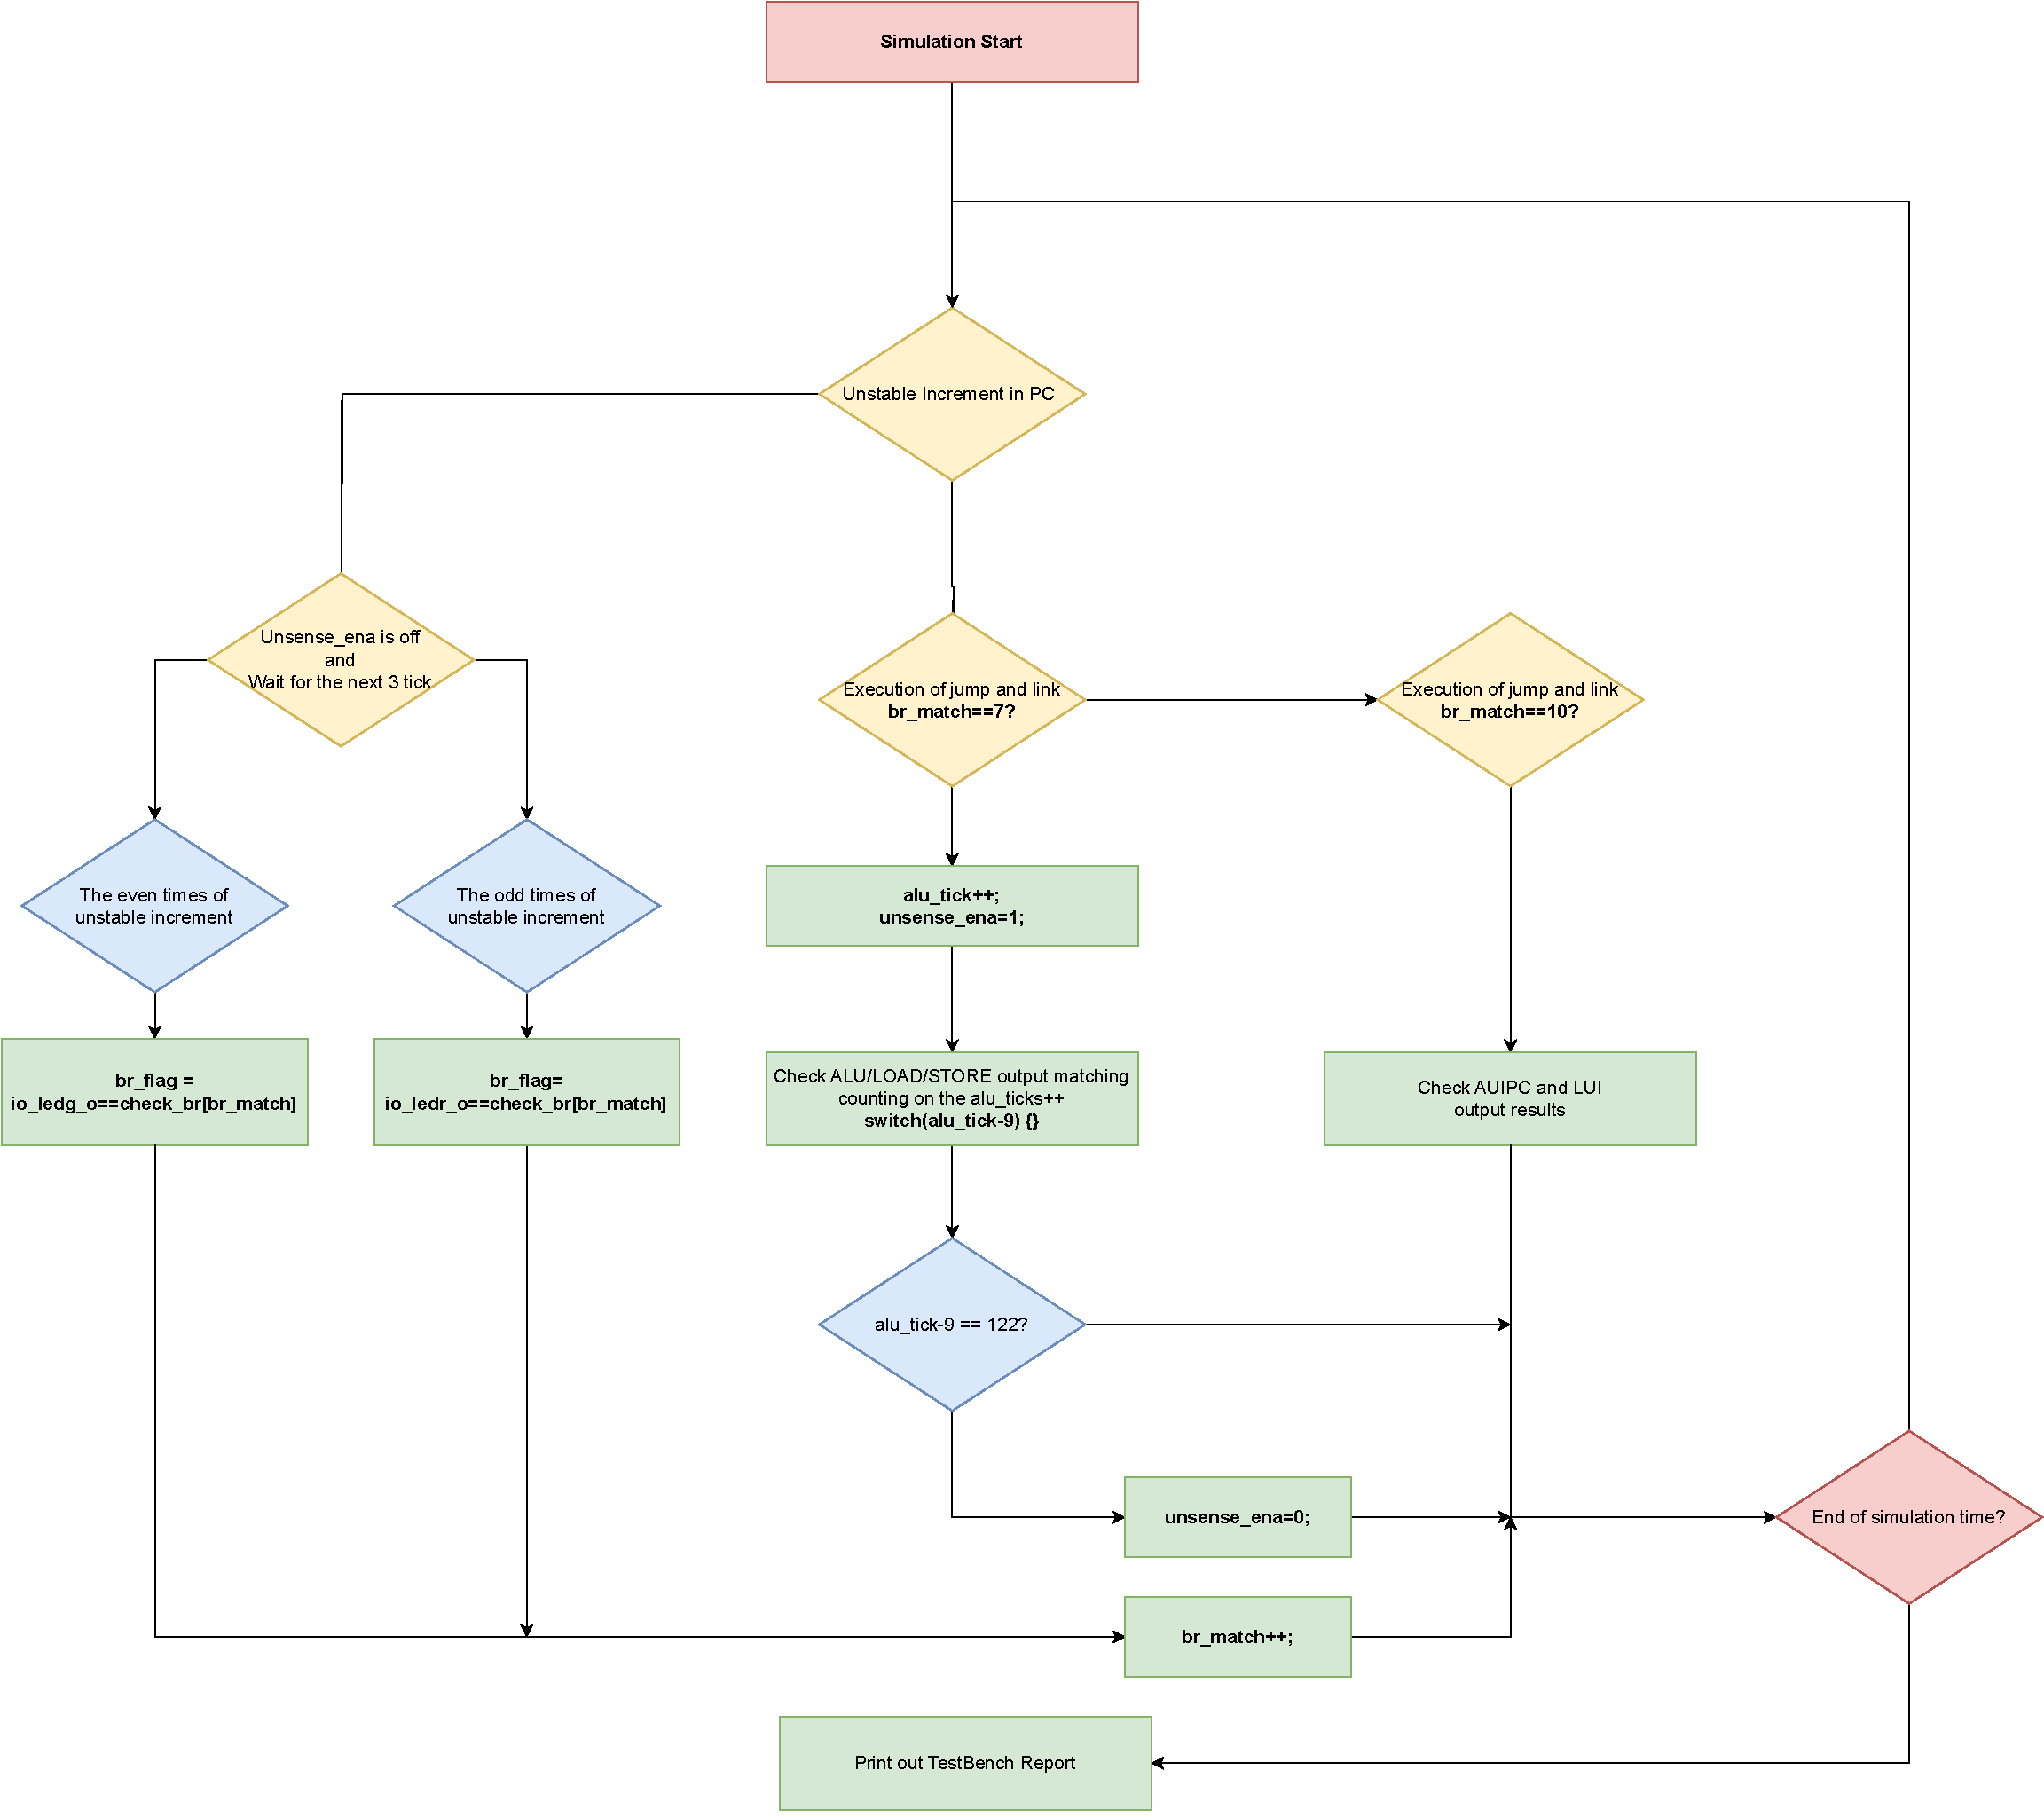
\includegraphics[trim=0cm 0cm 0cm 0cm,clip,width=.9\textwidth]{images/testbench_af.drawio.pdf}
    \caption{The overall algorithm flows of verification strategies}
    \end{center}
\end{figure}

 \begin{figure}[H]
    \begin{center}
    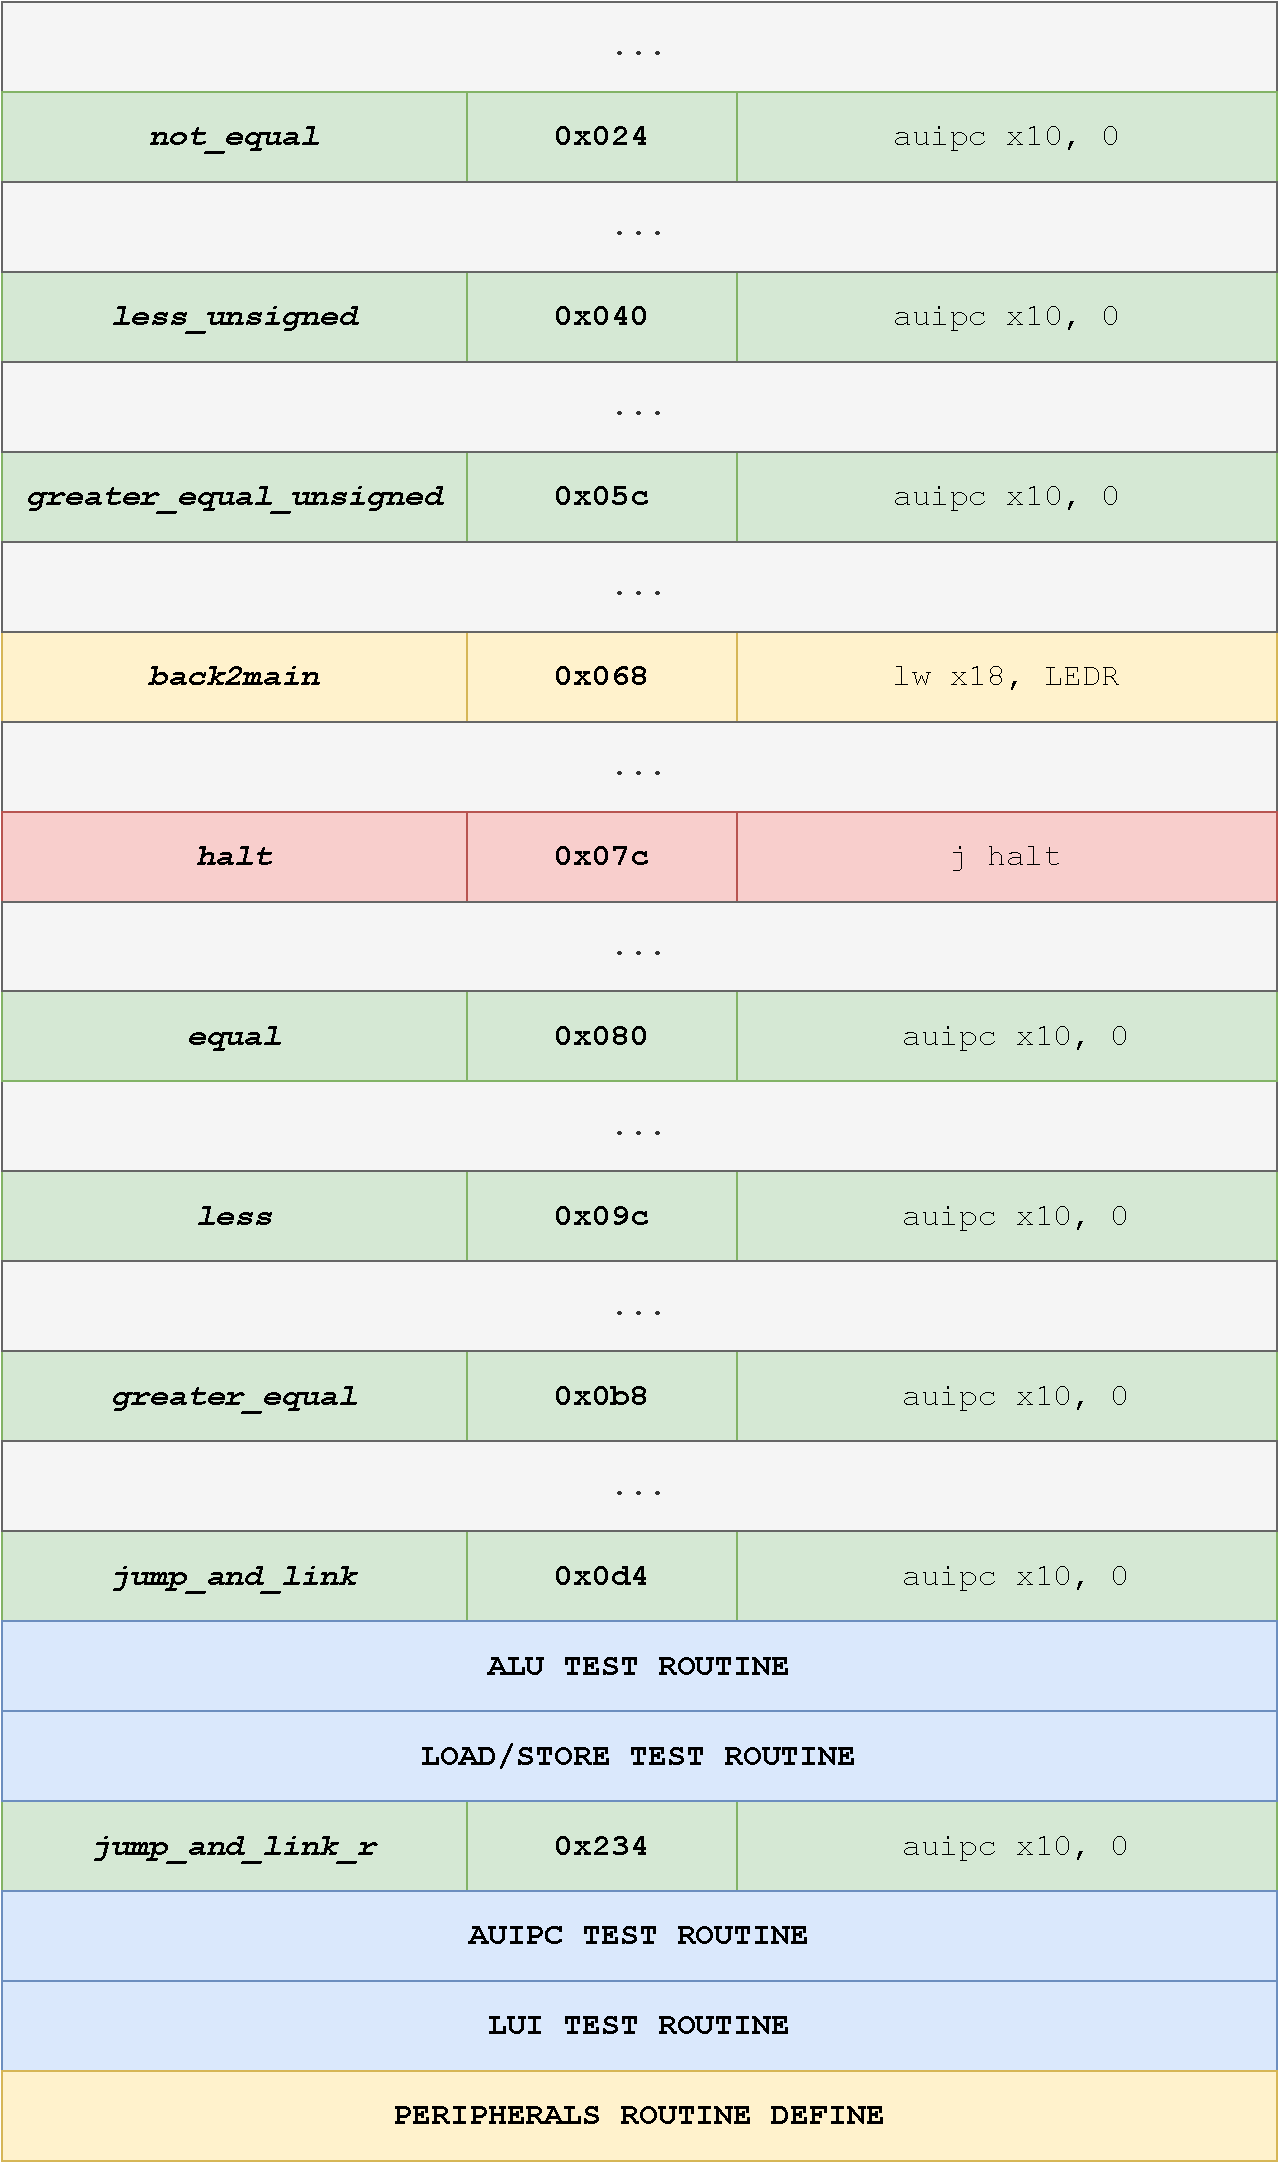
\includegraphics[trim=0cm 0cm 0cm 0cm,clip,width=.88\textwidth]{images/testbench_struct_asm.drawio.pdf}
    \caption{An general observation of branch/jump peripheral outputting}
    \end{center}
\end{figure}
% \subsection{Branch and Jump Verification}

In reference to the software testbench, as illustrated in the figure below, it follows a similar implementation approach to the assembly programs. The testbench is executed in accordance with a predefined flow, which encompasses both branch/jump and load/store/ALU testbench segments. Our initial focus lies on the branch/jump testbench, as indicated. Following the algorithm flow diagram, the C++ testbench program diligently monitors any fluctuations in the PC address, specifically tracking instances where the address increment is not the standard 4, indicative of a jump or branch instruction. When such changes are detected, the testbench promptly triggers a notification and counts three clock cycles after the alteration. This three-cycle interval aligns with the time required for the result to be processed and displayed on the output peripheral, in this case, LEDs. It's worth mentioning that every change in even clock cycles results in the jump/branch address being displayed on LEDs designated as \texttt{LEDG}, while changes occurring in odd cycles are conveyed through LEDs marked as \texttt{LEDR}. Once the necessary waiting period is reached, we will proceed to compare whether the jump address aligns with the predefined jump/branch addresses, as specified in the table provided.

\begin{table}[H]
\centering
\caption{A summary interface of software testing and hardware programming}
\begin{tabular}{|c|ccc|c|}
\hline
\textbf{Branch} & \multicolumn{1}{c|}{\textbf{Number A}} & \multicolumn{1}{c|}{\textbf{Number B}} & \textbf{Comparision flag} & \textbf{\begin{tabular}[c]{@{}c@{}}Destination\end{tabular}} \\ \hline
0               & \multicolumn{1}{c|}{0x0000000A}        & \multicolumn{1}{c|}{0x0000000A}        & Equal                     & 0x080                                                                       \\ \hline
1               & \multicolumn{1}{c|}{0x0000000A}        & \multicolumn{1}{c|}{0xFFFFFFEC}        & Not equal                 & 0x024                                                                       \\ \hline
2               & \multicolumn{1}{c|}{0xFFFFFFEC}        & \multicolumn{1}{c|}{0x0000000A}        & Less than                 & 0x09C                                                                       \\ \hline
3               & \multicolumn{1}{c|}{0x0000000A}        & \multicolumn{1}{c|}{0xFFFFFFEC}        & Less than (Unsigned)      & 0x040                                                                       \\ \hline
4               & \multicolumn{1}{c|}{0x0000000A}        & \multicolumn{1}{c|}{0xFFFFFFEC}        & Greater than              & 0x0B8                                                                       \\ \hline
5               & \multicolumn{1}{c|}{0xFFFFFFEC}        & \multicolumn{1}{c|}{0x0000000A}        & Greater than (Unsigned)   & 0x05C                                                                        \\ \hline
6               & \multicolumn{3}{c|}{Jump and Link}                                                                          & 0x0D4                                                                       \\ \hline
7               & \multicolumn{3}{c|}{Back   to Main}                                                                         & 0x068                                                                       \\ \hline
8               & \multicolumn{3}{c|}{Jump and Link By Register}                                                              & 0x234                                                                       \\ \hline
9               & \multicolumn{3}{c|}{Halt}                                                                                   & 0x07C                                                                       \\ \hline
\end{tabular}
\end{table}
% Recall from the assembly program, we've introduced two data variables, \texttt{a\_no: .word 0x0000000A} and \texttt{b\_no: .word 0xFFFFFFEC}, meticulously chosen to effectively illustrate the distinctions between unsigned and signed comparisons. Following the sequence provided in the table, the order of unpredictable changes serves as an indicator of the specific branch/jump instructions being executed, namely \texttt{beq, bne, blt, bltu, bgt, bgtu, jal, ret\_jal, jalr, and ret\_jalr}, respectively. Notably, for \texttt{jal and jal\_ret}, as well as \texttt{jalr and jal\_ret}, an additional branch/jump instruction is required to transition to the main programs. The results of these comparisons are systematically stored in an array variable called \texttt{br\_flag}, serving as a clear indicator of whether they resulted in a match or not. This \texttt{br\_flag} is integral for generating the Testbench Report at the conclusion of the simulation runtime. Furthermore, the algorithm is equipped to detect changes after the execution of a jal jump (i.e, \texttt{br\_match = 7}), triggering an independent count variable that plays a vital role in the ALU/LOAD/STORE Testbench. This is particularly valuable, considering the potential need to count a substantial number of clock ticks from the main programs, which might be more time-consuming compared to routine \texttt{jal} programs. The mechanism for sensing changes in branch/jump instructions only remains active until the completion of our ALU/LOAD/STORE programs.


% \subsection{ALU verification}
The Branch/Jump Testbench is responsible for testing all branch (B-type) and jump-related (J-type) instructions, with the results being recorded in an array variable named \texttt{br\_flag}. Similarly, the ALU/Load/Store Testbench is dedicated to testing all ALU (R-type, I-type), load (load I-type), store (S-type) and U-type instructions, and its results are stored in an array variable named \texttt{alu\_flag}. These arrays, combined with the \texttt{br\_flag}, play a pivotal role in generating the Testbench report. This report is generated by evaluating the boolean variables contained within the arrays and utilizing the \texttt{pass\_message} functions to communicate the test outcomes at the conclusion of the simulation runtime.

% The testbench is designed to encompass a diverse set of test cases, each catering to different instruction formats, including I-type and R-type instructions. Additionally, it tests a range of load and store instructions, such as \texttt{LW}, \texttt{SW}, \texttt{LHU}, \texttt{SH}, \texttt{LBU}, \texttt{SB} (Store Byte Unsigned), \texttt{BEQ}, \texttt{BNE}, \texttt{BLT}, \texttt{BEQ} , \texttt{BNE} (Branch Not Equal), \texttt{BLT}, \texttt{BLTU}, BGT (Branch Greater Than), and BGTU (Branch Greater Than Unsigned). The list of test cases in the \texttt{cpp} testbench is generated based on the instruction format.
\begin{minted}{text} 
> SIMULATING ----------------  
::PASSED:: Successful Test w.    LW, SW     Instructions
::PASSED:: Successful Test w.    ADD        Instructions
::PASSED:: Successful Test w.    SUB        Instructions
::PASSED:: Successful Test w.    XOR        Instructions
::PASSED:: Successful Test w.    OR         Instructions
::PASSED:: Successful Test w.    AND        Instructions
::PASSED:: Successful Test w.    SLL        Instructions
::PASSED:: Successful Test w.    SRL        Instructions
::PASSED:: Successful Test w.    SLT        Instructions
::PASSED:: Successful Test w.    SLTU       Instructions
::PASSED:: Successful Test w.    SRA        Instructions
::PASSED:: Successful Test w.    ADDI       Instructions
::PASSED:: Successful Test w.    XORI       Instructions
::PASSED:: Successful Test w.    ORI        Instructions
::PASSED:: Successful Test w.    ANDI       Instructions
::PASSED:: Successful Test w.    SLLI       Instructions
::PASSED:: Successful Test w.    SRLI       Instructions
::PASSED:: Successful Test w.    SLTI       Instructions
::PASSED:: Successful Test w.    SLTIU      Instructions
::PASSED:: Successful Test w.    SRAI       Instructions
::PASSED:: Successful Test w.    LHU, SH    Instructions
::PASSED:: Successful Test w.    LBU, SB    Instructions
::PASSED:: Successful Test w.    LH, SH     Instructions
::PASSED:: Successful Test w.    LB, SB     Instructions
::PASSED:: Successful Test w.    BEQ        Instructions
::PASSED:: Successful Test w.    BNE        Instructions
::PASSED:: Successful Test w.    BLT        Instructions
::PASSED:: Successful Test w.    BLTU       Instructions
::PASSED:: Successful Test w.    BGT        Instructions
::PASSED:: Successful Test w.    BGTU       Instructions
::PASSED:: Successful Test w.    JAL        Instructions
::PASSED:: Successful Test w.    JALR       Instructions
::PASSED:: Successful Test w.    LUI        Instructions
::PASSED:: Successful Test w.    AUIPC      Instructions
\end{minted}


%  \begin{figure}[H]
%     \begin{center}
%     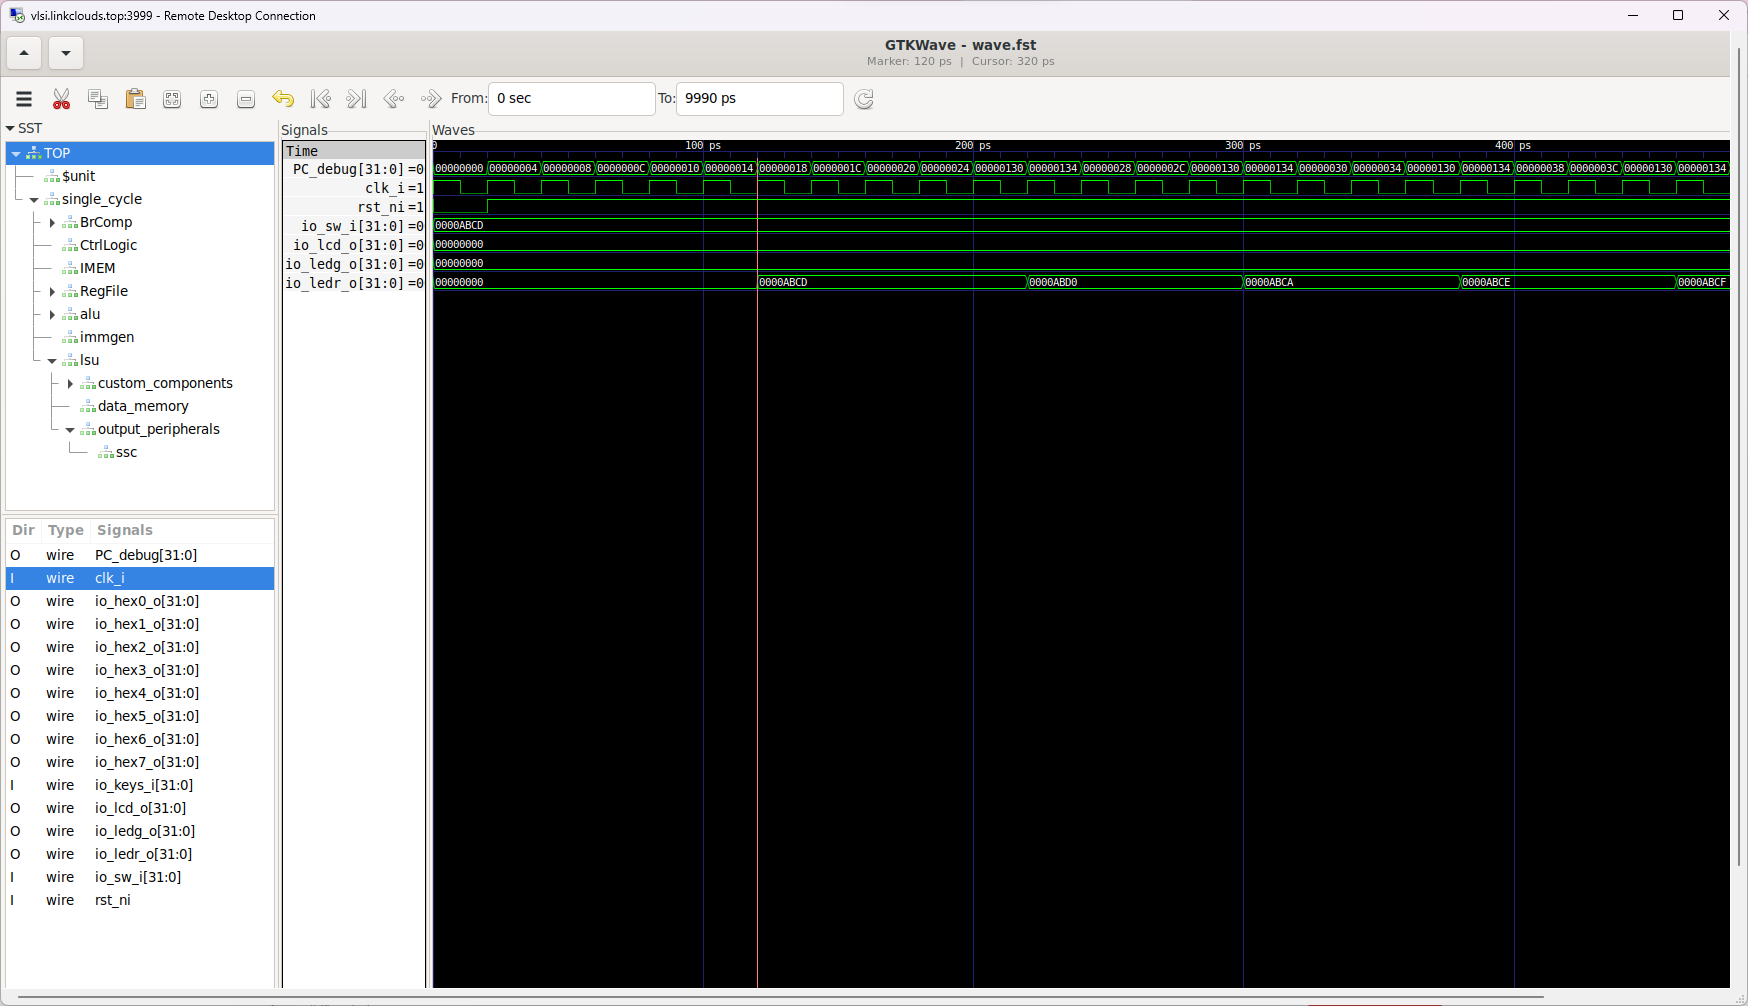
\includegraphics[trim=7.5cm 18cm 1cm 3cm,clip,width=\textwidth]{images/sim1}
%     \caption{The waveform of \texttt{LW, SW} instruction}
%     \end{center}
% \end{figure}
% At \texttt{PC\_debug = 0x00000000}, the \texttt{LW} instruction is pass when loading data (\texttt{io\_ledr\_o} = \texttt{0x0000ABCD}) from memory into a register. At \texttt{PC\_debug = 0x00000018}, the \texttt{SW} instruction is pass when storing data (\texttt{io\_ledr\_o} = \texttt{0x0000ABCD}) from a register into memory.

%  \begin{figure}[H]
%     \begin{center}
%     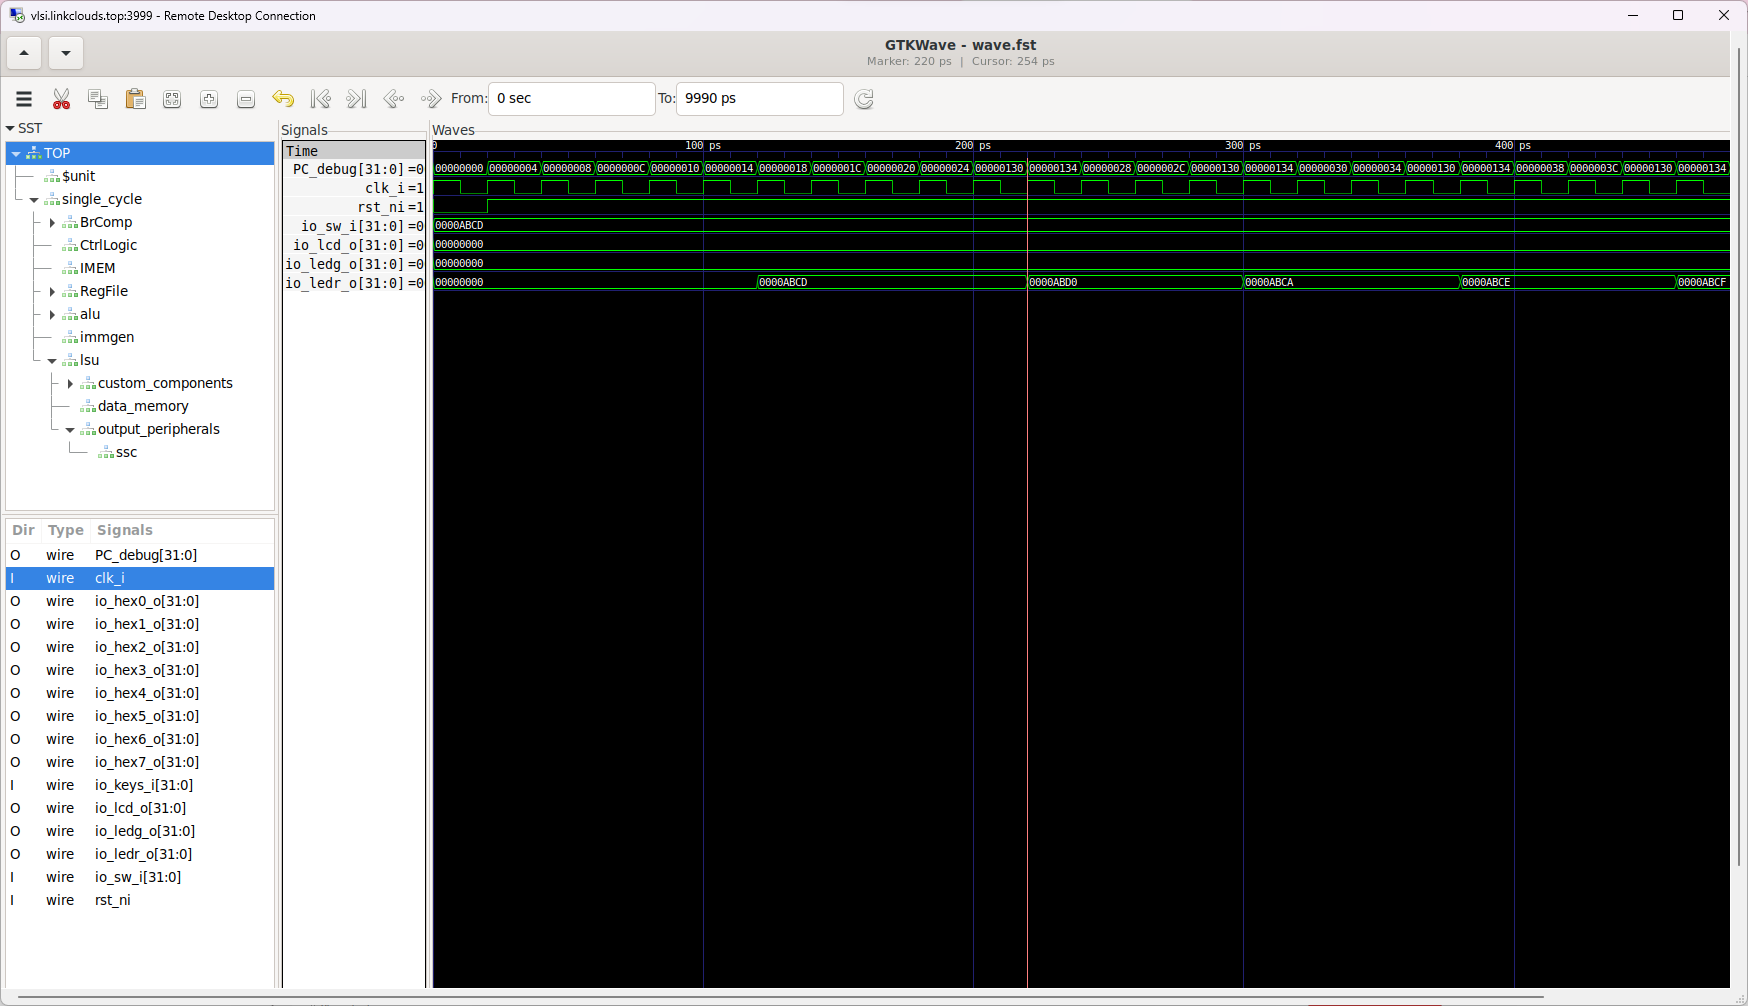
\includegraphics[trim=7.5cm 18cm 1cm 3cm,clip,width=\textwidth]{images/sim2}
%     \caption{The waveform of \texttt{add} instruction}
%     \end{center}
% \end{figure}
% At \texttt{PC\_debug = 0x00000134}, the \texttt{add} instruction is pass (\texttt{0x0000ABCD + 0x00000003 = 0x0000ABD0}) with \texttt{io\_ledr\_o} = \texttt{0x0000ABD0}.
%  \begin{figure}[H]
%     \begin{center}
%     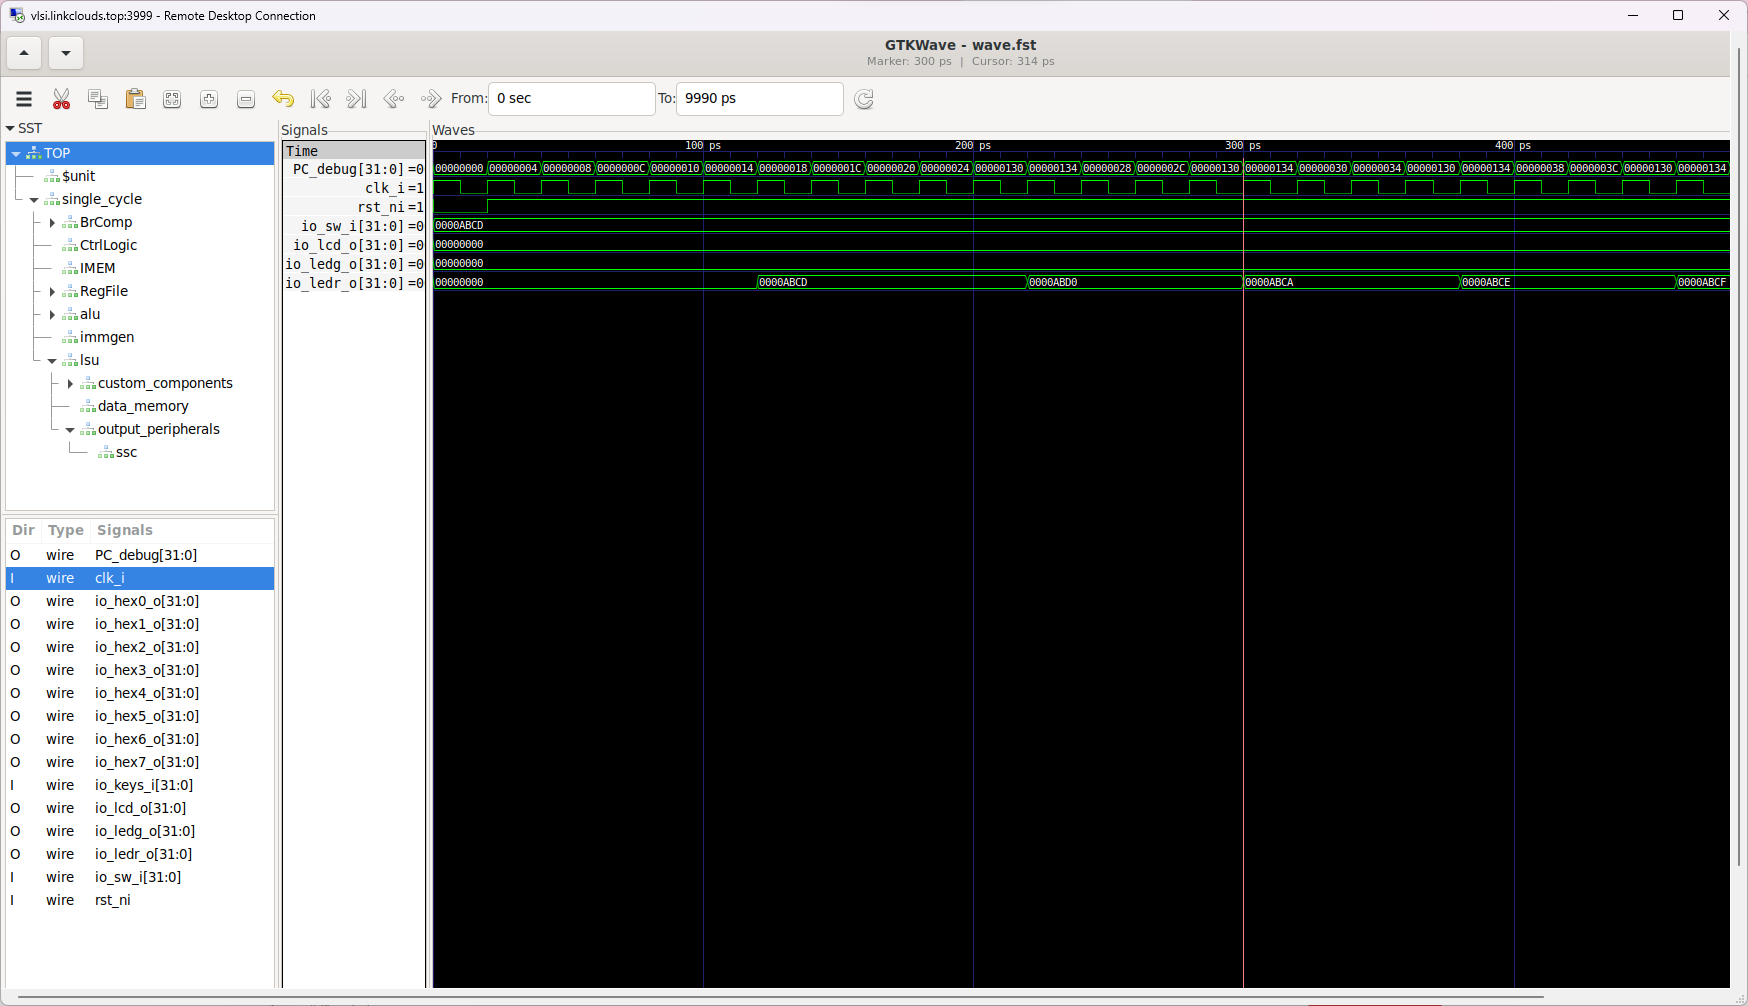
\includegraphics[trim=7.5cm 18cm 1cm 3cm,clip,width=\textwidth]{images/sim3}
%     \caption{The waveform of \texttt{sub} instruction}
%     \end{center}
% \end{figure}
% At \texttt{PC\_debug = 0x00000134}, the \texttt{sub} instruction is pass (\texttt{0x0000ABCD - 0x00000003 = 0x0000ABCA}) with \texttt{io\_ledr\_o} = \texttt{0x0000ABCA}.
%  \begin{figure}[H]
%     \begin{center}
%     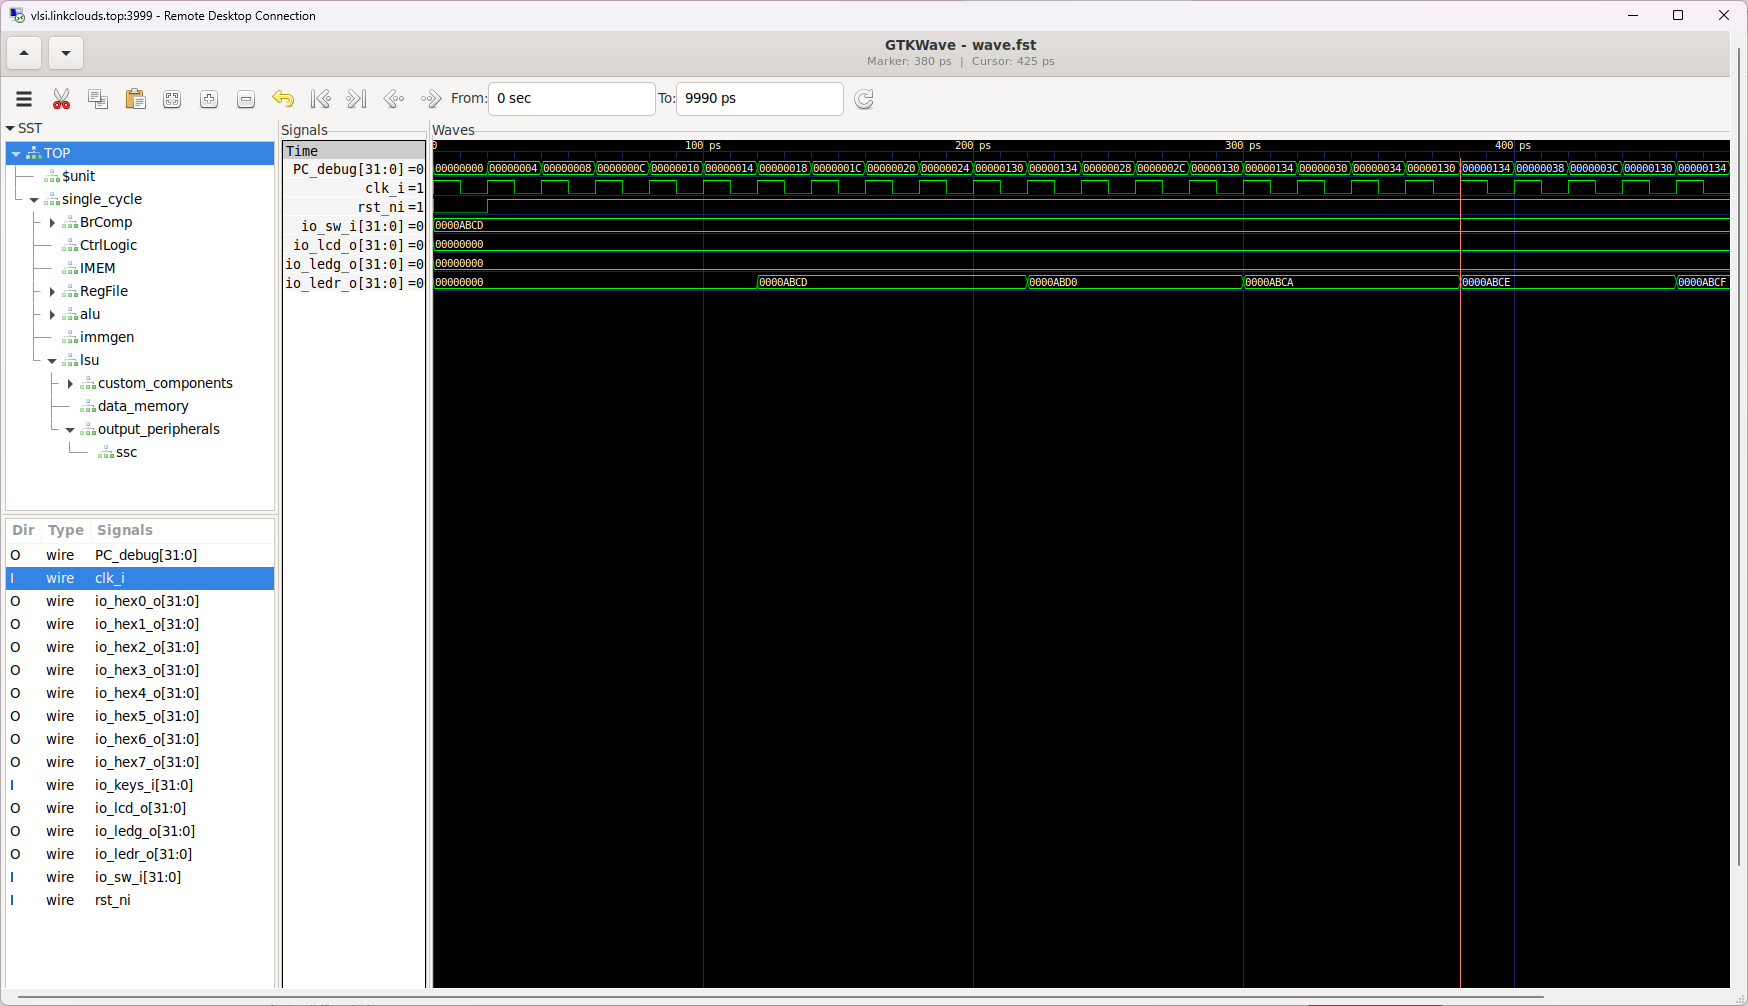
\includegraphics[trim=7.5cm 18cm 1cm 3cm,clip,width=\textwidth]{images/sim4}
%     \caption{The waveform of \texttt{xor} instruction}
%     \end{center}
% \end{figure}
% At \texttt{PC\_debug = 0x00000134}, the \texttt{xor} instruction is pass (\texttt{0x0000ABCD  $\oplus$ 0x00000003 = 0x0000ABCE}) with \texttt{io\_ledr\_o} = \texttt{0x0000ABCE}.
%  \begin{figure}[H]
%     \begin{center}
%     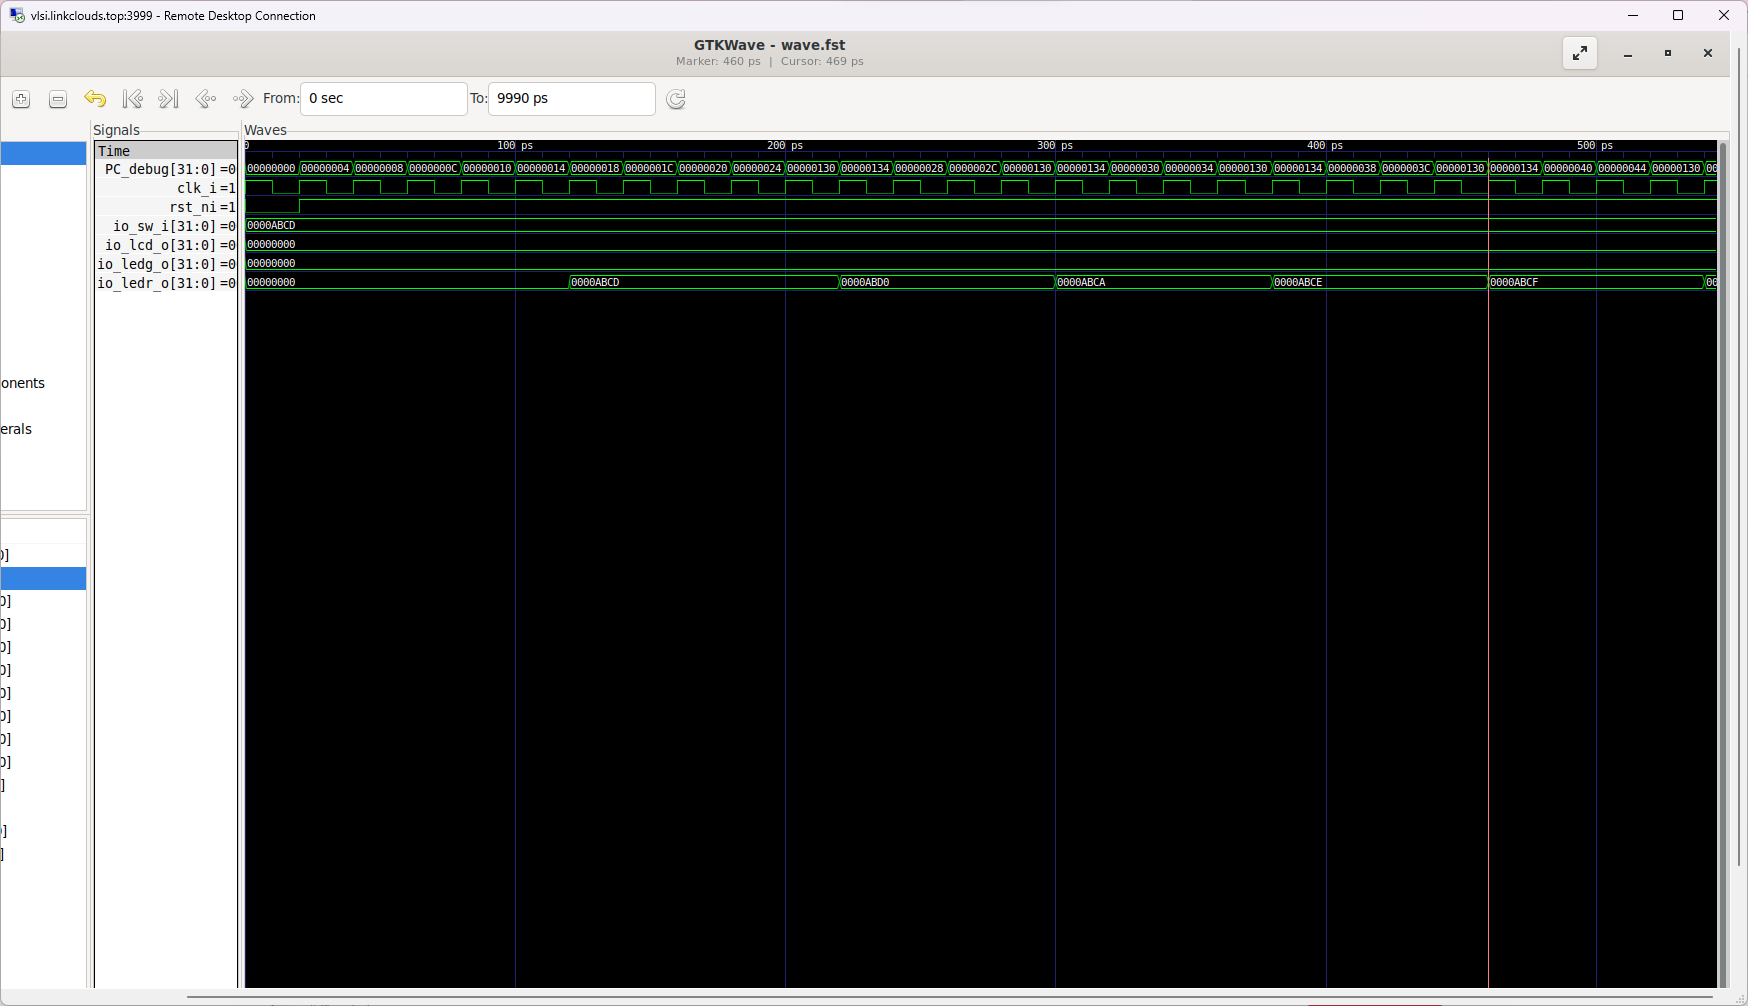
\includegraphics[trim=2.5cm 18cm 1cm 3cm,clip,width=\textwidth]{images/sim5}
%     \caption{The waveform of \texttt{or} instruction}
%     \end{center}
% \end{figure}
% At \texttt{PC\_debug = 0x00000134}, the \texttt{or} instruction is pass (\texttt{0x0000ABCD  $\vee$ 0x00000003 = 0x0000ABCF}) with \texttt{io\_ledr\_o} = \texttt{0x0000ABCF}.

%  \begin{figure}[H]
%     \begin{center}
%     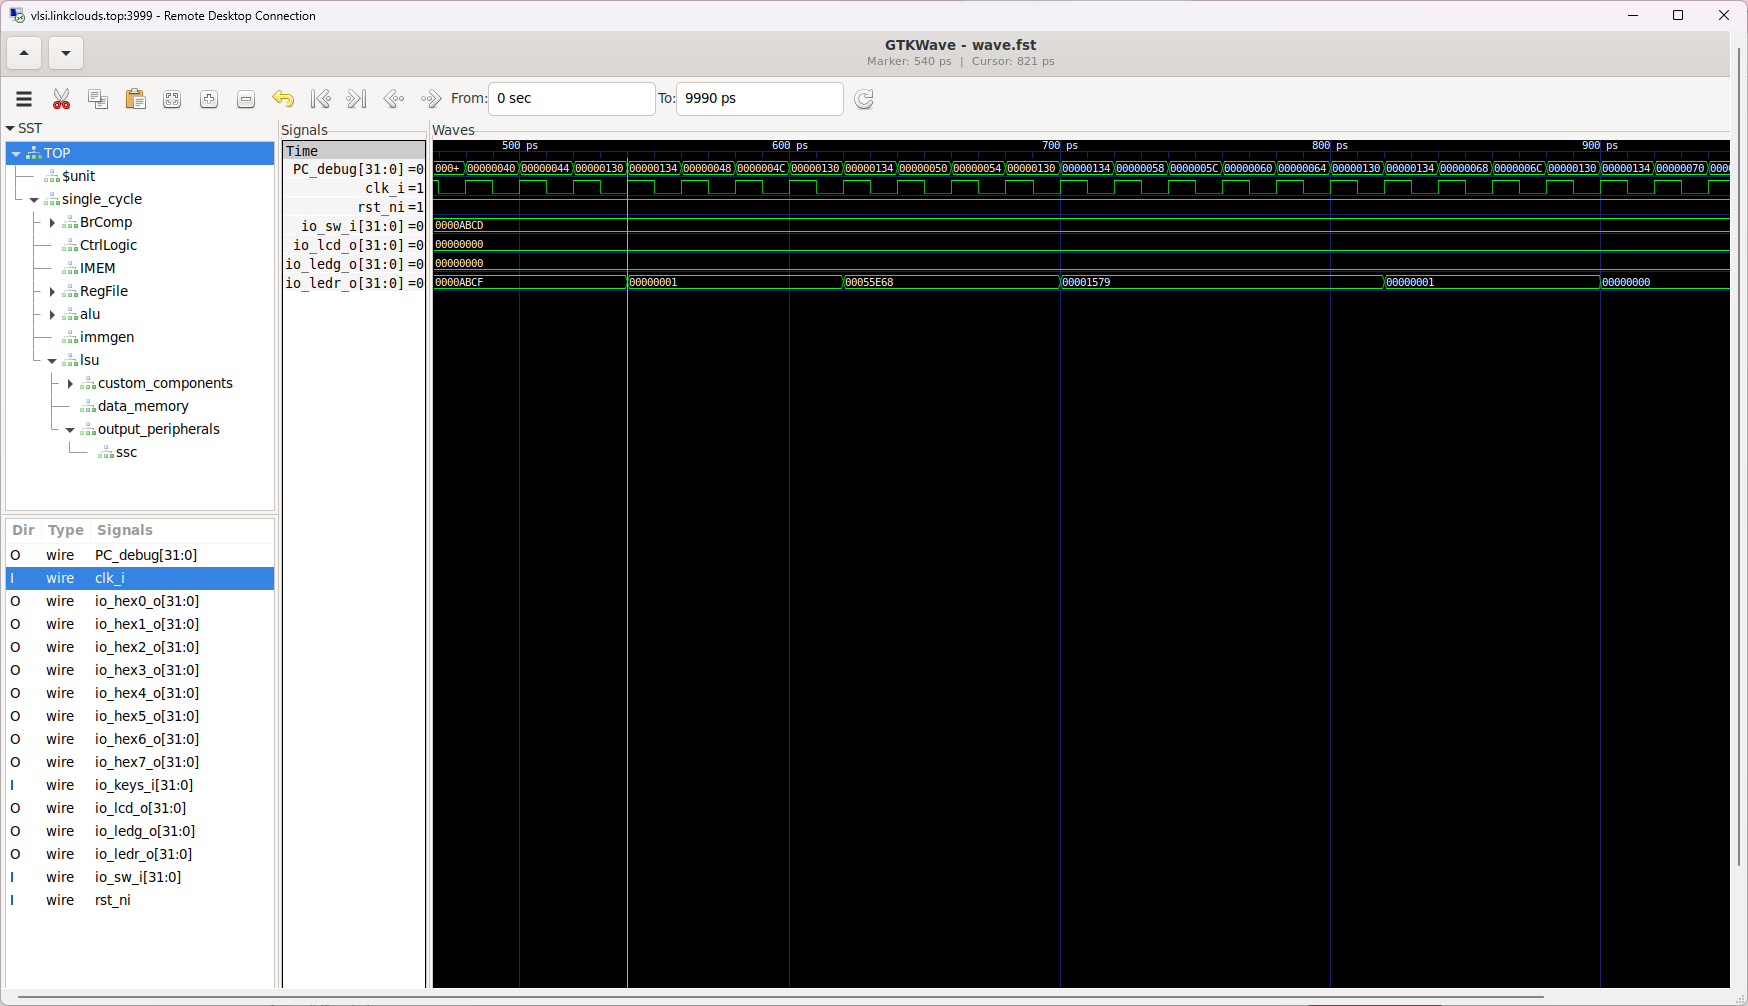
\includegraphics[trim=7.5cm 18cm 1cm 3cm,clip,width=\textwidth]{images/sim6}
%     \caption{The waveform of \texttt{and} instruction}
%     \end{center}
% \end{figure}
% At \texttt{PC\_debug = 0x00000134}, the \texttt{or} instruction is pass (\texttt{0x0000ABCD $\wedge$ 0x00000003 = 0x00000001}) with \texttt{io\_ledr\_o} = \texttt{0x00000001}.

%  \begin{figure}[H]
%     \begin{center}
%     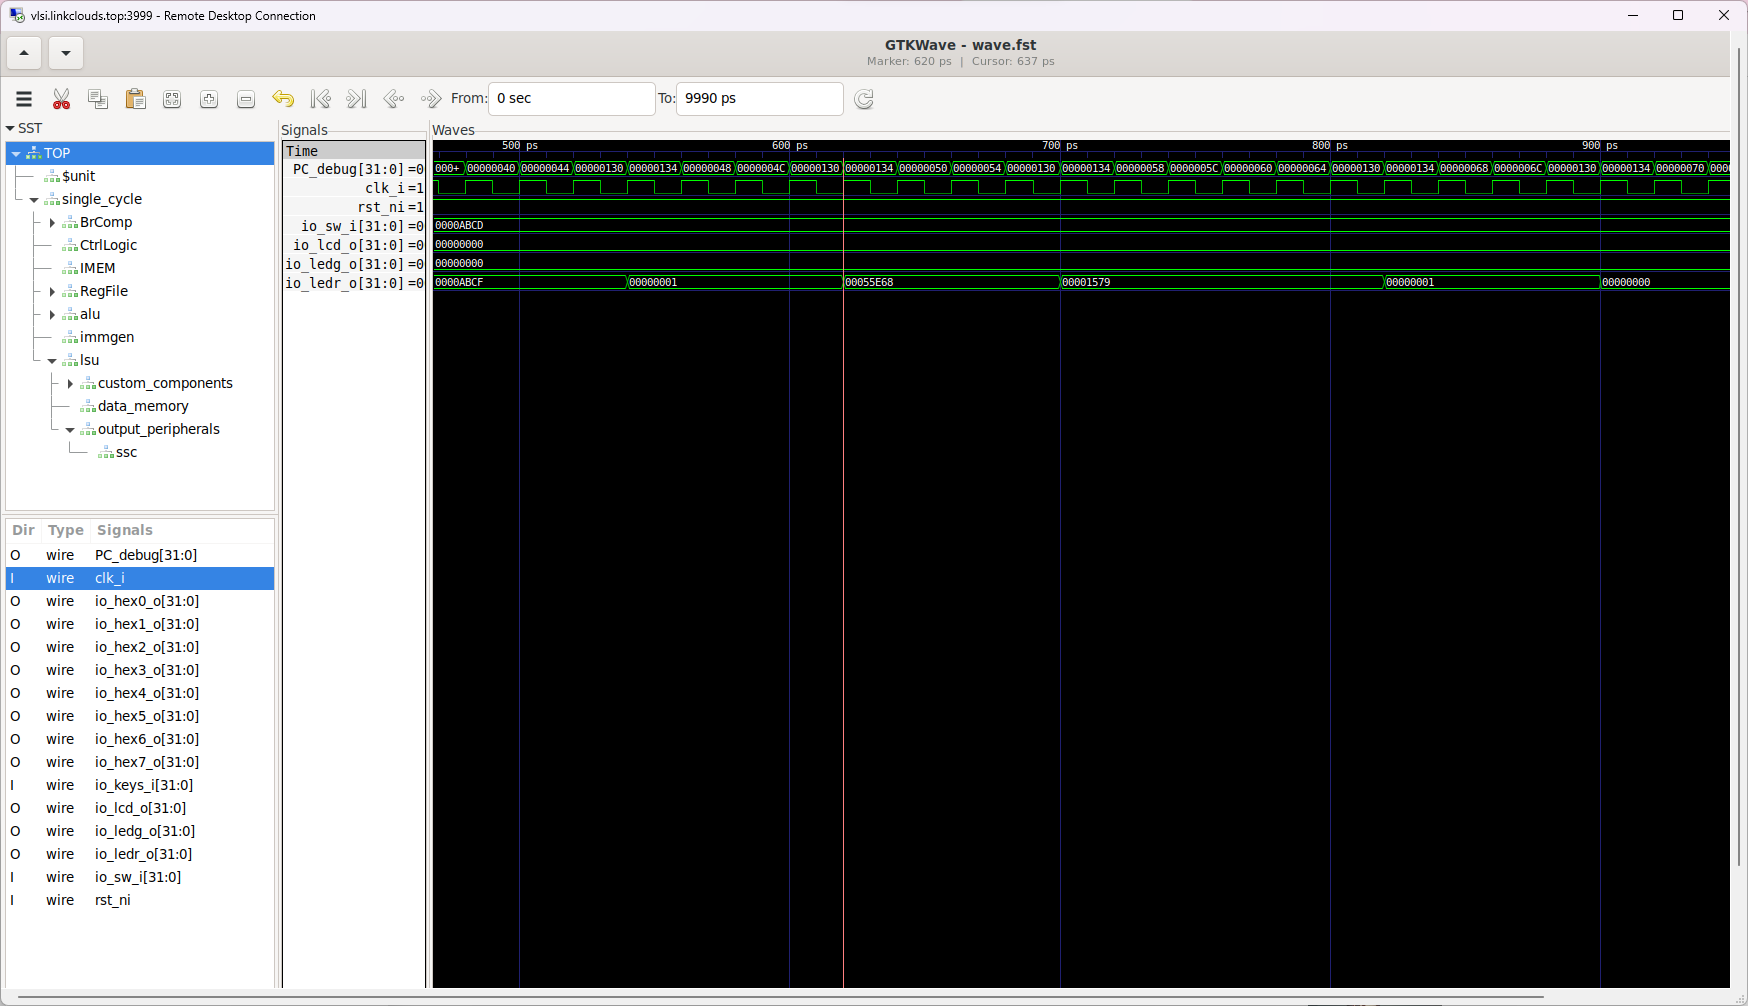
\includegraphics[trim=7.5cm 18cm 1cm 3cm,clip,width=\textwidth]{images/sim7}
%     \caption{The waveform of \texttt{sll} instruction}
%     \end{center}
% \end{figure}
% At \texttt{PC\_debug = 0x00000134}, the \texttt{sll} instruction is pass (\texttt{0x0000ABCD $\ll$ 0x00000003 = 0x00055E68}) with \texttt{io\_ledr\_o} = \texttt{0x00055E68}.

%  \begin{figure}[H]
%     \begin{center}
%     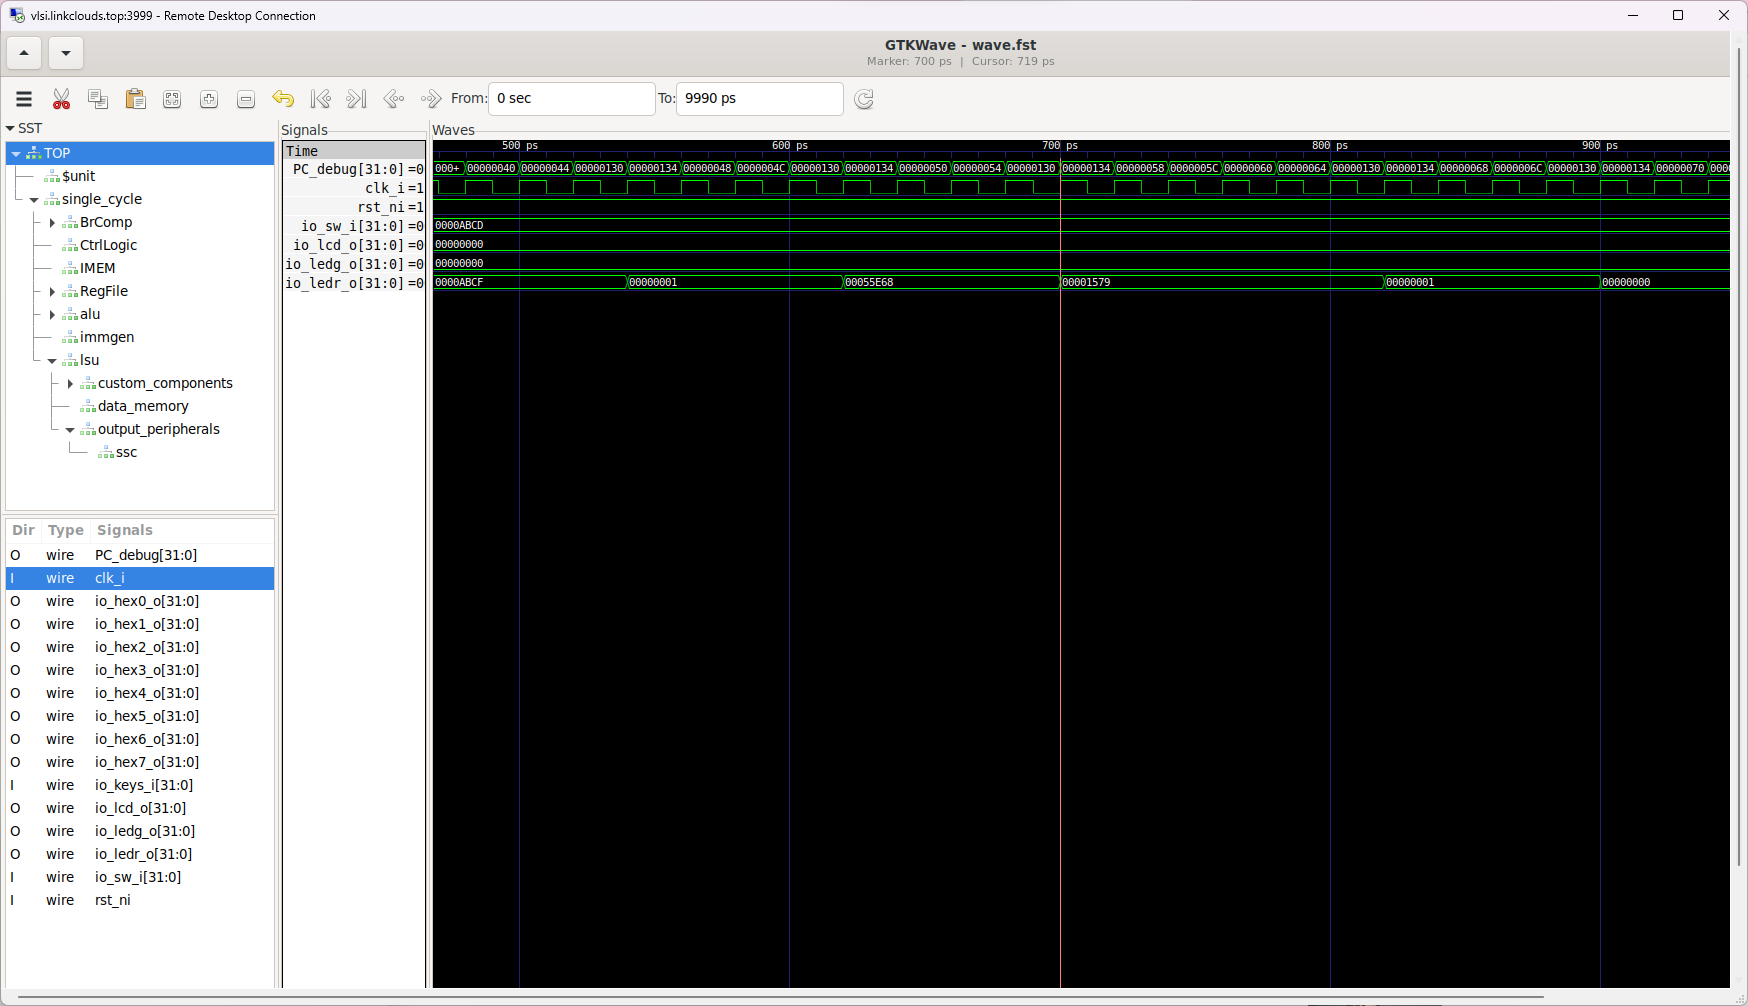
\includegraphics[trim=7.5cm 18cm 1cm 3cm,clip,width=\textwidth]{images/sim8}
%     \caption{The waveform of \texttt{srl} instruction}
%     \end{center}
% \end{figure}
% At \texttt{PC\_debug = 0x00000134}, the \texttt{srl} instruction is pass (\texttt{0x0000ABCD $\gg$ 0x00000003 = 0x00000001}) with \texttt{io\_ledr\_o} = \texttt{0x000001579}.

%  \begin{figure}[H]
%     \begin{center}
%     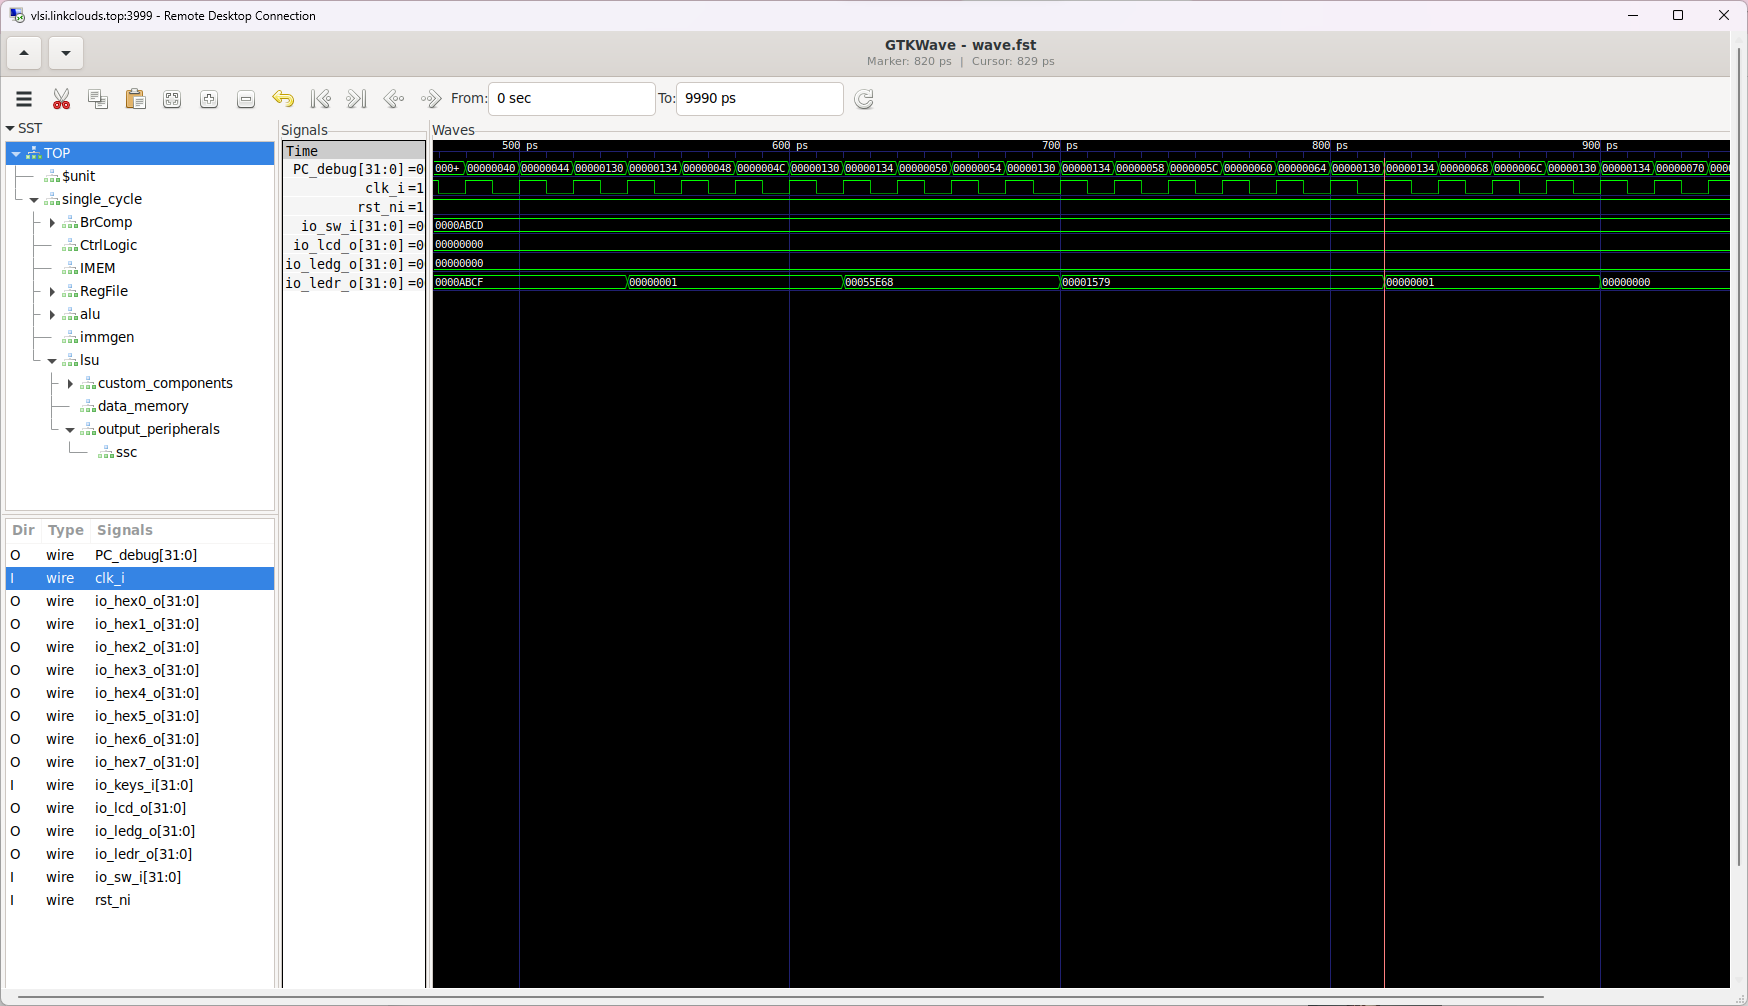
\includegraphics[trim=7.5cm 18cm 1cm 3cm,clip,width=\textwidth]{images/sim9}
%     \caption{The waveform of \texttt{slt} instruction}
%     \end{center}
% \end{figure}
% At \texttt{PC\_debug = 0x00000134}, the \texttt{slt} instruction is pass (\texttt{0x0000ABCD $<$ 0x00000003 = 0x00000001}) with \texttt{io\_ledr\_o} = \texttt{0x00000001}.

%  \begin{figure}[H]
%     \begin{center}
%     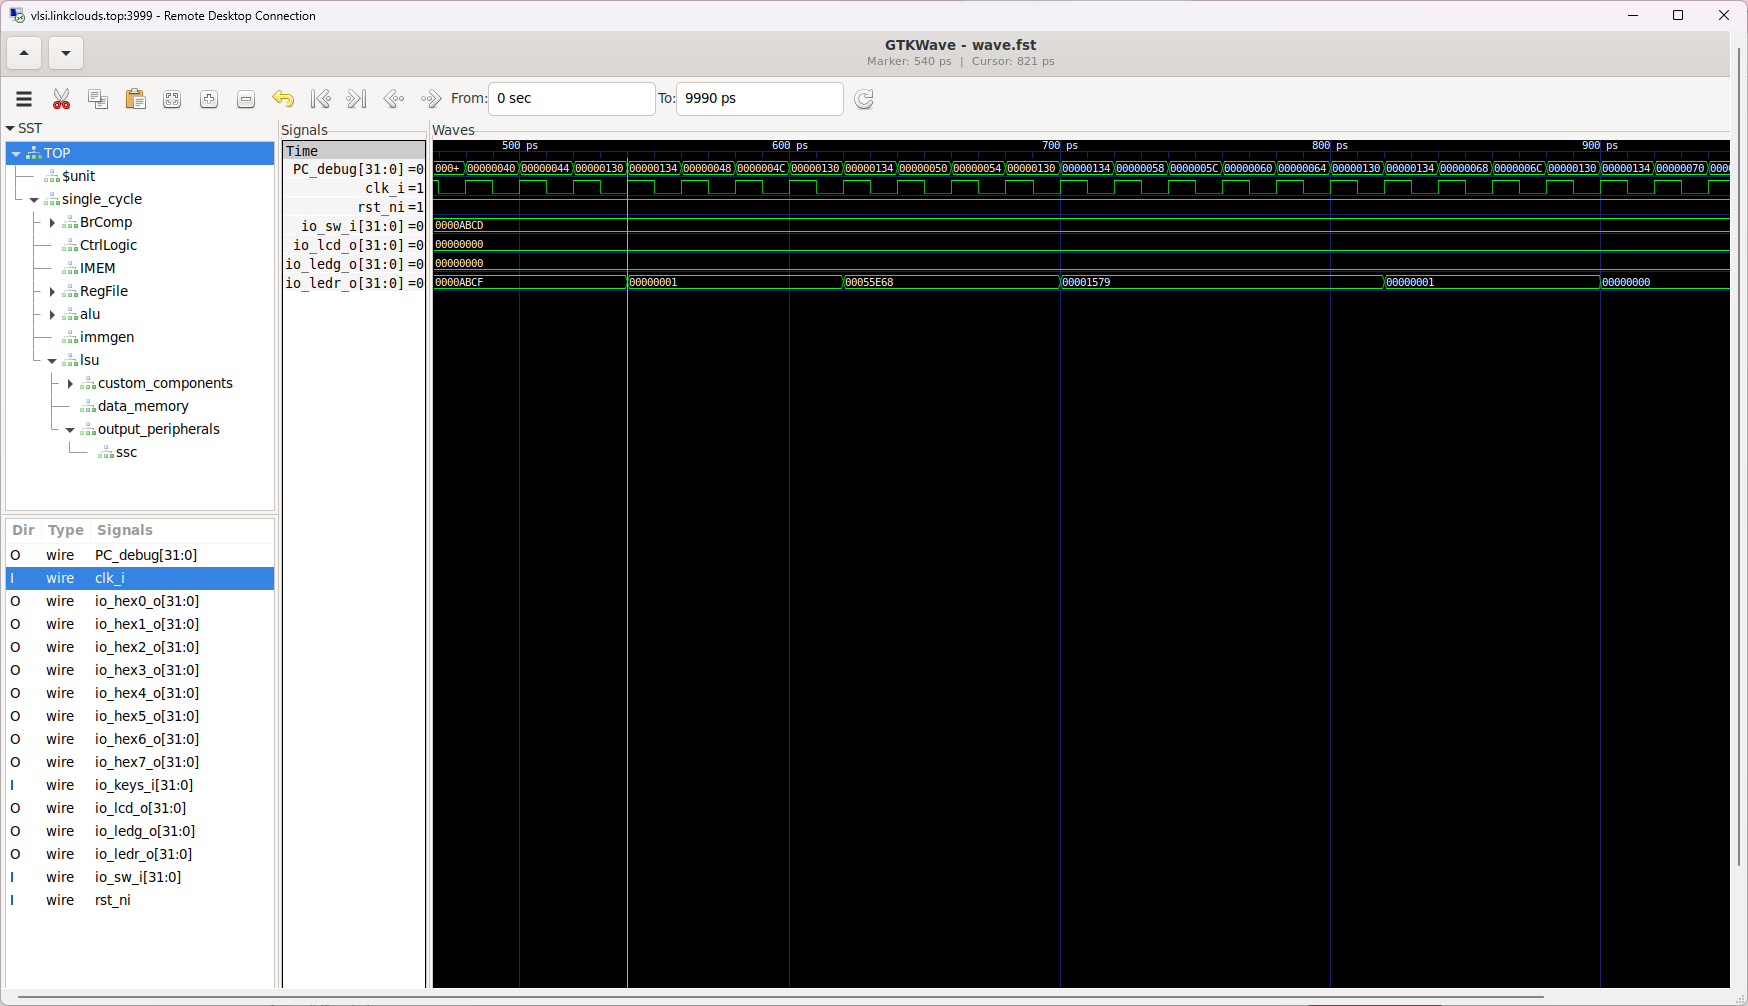
\includegraphics[trim=7.5cm 18cm 1cm 3cm,clip,width=\textwidth]{images/sim6}
%     \caption{The waveform of \texttt{sltu} instruction}
%     \end{center}
% \end{figure}
% At \texttt{PC\_debug = 0x00000134}, the \texttt{sltu} instruction is pass (\texttt{0xFFFFABCD $<$ 0x00000003 = 0x00000000}) with \texttt{io\_ledr\_o} = \texttt{0x00000000}.

\section{Run test programs}
\subsection{Factorial Calculation}
\begin{figure}[H]
    \centering
    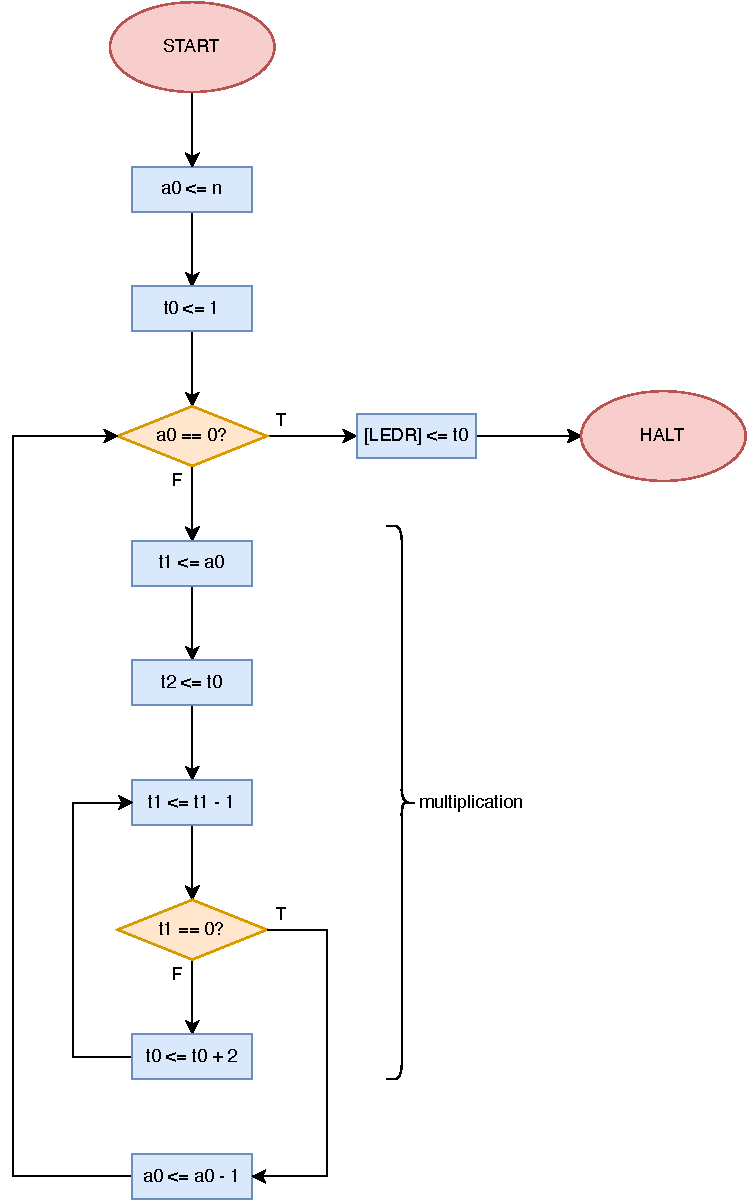
\includegraphics[width=.7\textwidth]{images/flowchart/factorial.pdf}
    \caption{Program Flow for calculating factorial}
\end{figure}

Assembly code for the processor is stored in the Instruction Memory (IMEM), while the value of $n$ is stored in the Data Memory (DMEM). The processor calculates the result and outputs it on the LEDR. The testbench is specifically designed to test the processor for $n$ values ranging from 0 to 12. In the testbench, the factorial is computed in C, and the result is then compared with the output on the \texttt{LEDR}. The test results are displayed as follows. This program utilized \texttt{add}, \texttt{addi}, \texttt{lw}, \texttt{sw}, \texttt{beq}, \texttt{jal}, \texttt{jalr} and \texttt{auipc} instructions.

\begin{minted}{text}
   0 -- N= 0, expected: 1
  90 --    LEDR output: 1 => PASSED
   0 -- N= 1, expected: 1
 180 --    LEDR output: 1 => PASSED
   0 -- N= 2, expected: 2
 310 --    LEDR output: 2 => PASSED
   0 -- N= 3, expected: 6
 480 --    LEDR output: 6 => PASSED
   0 -- N= 4, expected: 24
 690 --    LEDR output: 24 => PASSED
   0 -- N= 5, expected: 120
 940 --    LEDR output: 120 => PASSED
   0 -- N= 6, expected: 720
1230 --    LEDR output: 720 => PASSED
   0 -- N= 7, expected: 5040
1560 --    LEDR output: 5040 => PASSED
   0 -- N= 8, expected: 40320
1930 --    LEDR output: 40320 => PASSED
   0 -- N= 9, expected: 362880
2340 --    LEDR output: 362880 => PASSED
   0 -- N=10, expected: 3628800
2790 --    LEDR output: 3628800 => PASSED
   0 -- N=11, expected: 39916800
3280 --    LEDR output: 39916800 => PASSED
   0 -- N=12, expected: 479001600
3810 --    LEDR output: 479001600 => PASSED
\end{minted}

All test results have passed, indicating that the program and the CPU are operating correctly, at least for this specific program.

\subsection{Fibonacci Sequence Generator}
Another program has been developed to generate a Fibonacci sequence up to $n = 46$, and the resulting value is stored in the LEDR. A dedicated testbench has been created to calculate the Fibonacci sequence in C and compare it with the values on the LEDR, ensuring the correctness of the program's execution. This program utilized \texttt{add}, \texttt{addi}, \texttt{lw}, \texttt{sw}, \texttt{beq}, \texttt{jal} and \texttt{auipc} instructions.

\label{fibonacci}
\begin{figure}[H]
    \centering
    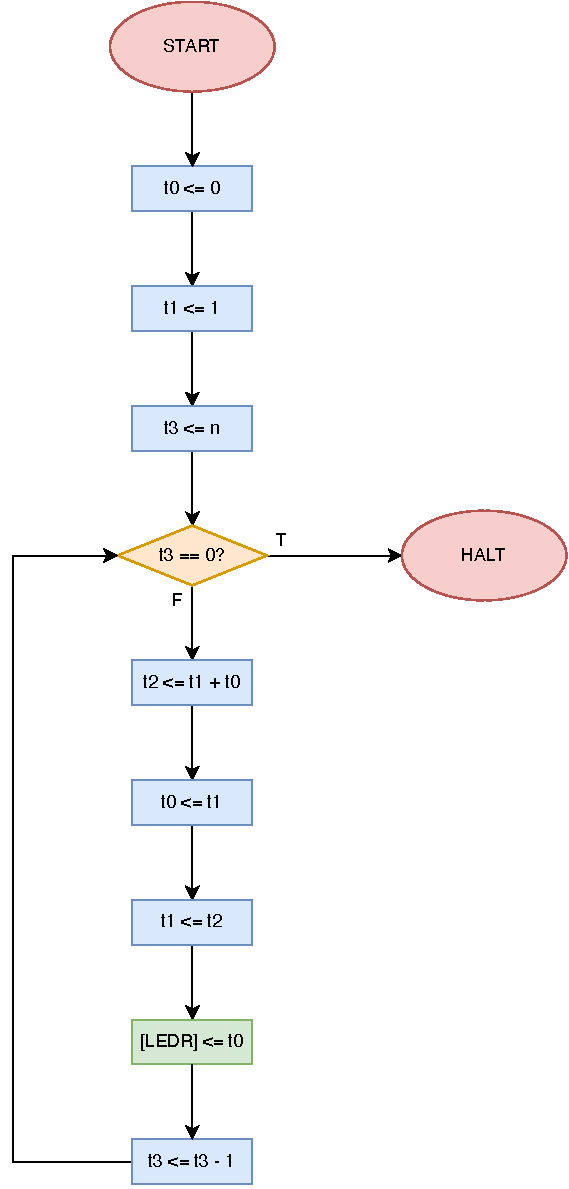
\includegraphics[width=.5\textwidth]{images/flowchart/fibonacci.pdf}
    \caption{Program flow for calculating Fibonacci sequence}
\end{figure}

\begin{minted}{text}
 120: n =  2, expected =          1, LEDR =          1 => PASSED
 260: n =  3, expected =          2, LEDR =          2 => PASSED
 330: n =  4, expected =          3, LEDR =          3 => PASSED
 400: n =  5, expected =          5, LEDR =          5 => PASSED
 470: n =  6, expected =          8, LEDR =          8 => PASSED
 540: n =  7, expected =         13, LEDR =         13 => PASSED
 610: n =  8, expected =         21, LEDR =         21 => PASSED
 680: n =  9, expected =         34, LEDR =         34 => PASSED
 750: n = 10, expected =         55, LEDR =         55 => PASSED
 820: n = 11, expected =         89, LEDR =         89 => PASSED
 890: n = 12, expected =        144, LEDR =        144 => PASSED
 960: n = 13, expected =        233, LEDR =        233 => PASSED
1030: n = 14, expected =        377, LEDR =        377 => PASSED
1100: n = 15, expected =        610, LEDR =        610 => PASSED
1170: n = 16, expected =        987, LEDR =        987 => PASSED
1240: n = 17, expected =       1597, LEDR =       1597 => PASSED
1310: n = 18, expected =       2584, LEDR =       2584 => PASSED
1380: n = 19, expected =       4181, LEDR =       4181 => PASSED
1450: n = 20, expected =       6765, LEDR =       6765 => PASSED
1520: n = 21, expected =      10946, LEDR =      10946 => PASSED
1590: n = 22, expected =      17711, LEDR =      17711 => PASSED
1660: n = 23, expected =      28657, LEDR =      28657 => PASSED
1730: n = 24, expected =      46368, LEDR =      46368 => PASSED
1800: n = 25, expected =      75025, LEDR =      75025 => PASSED
1870: n = 26, expected =     121393, LEDR =     121393 => PASSED
1940: n = 27, expected =     196418, LEDR =     196418 => PASSED
2010: n = 28, expected =     317811, LEDR =     317811 => PASSED
2080: n = 29, expected =     514229, LEDR =     514229 => PASSED
2150: n = 30, expected =     832040, LEDR =     832040 => PASSED
2220: n = 31, expected =    1346269, LEDR =    1346269 => PASSED
2290: n = 32, expected =    2178309, LEDR =    2178309 => PASSED
2360: n = 33, expected =    3524578, LEDR =    3524578 => PASSED
2430: n = 34, expected =    5702887, LEDR =    5702887 => PASSED
2500: n = 35, expected =    9227465, LEDR =    9227465 => PASSED
2570: n = 36, expected =   14930352, LEDR =   14930352 => PASSED
2640: n = 37, expected =   24157817, LEDR =   24157817 => PASSED
2710: n = 38, expected =   39088169, LEDR =   39088169 => PASSED
2780: n = 39, expected =   63245986, LEDR =   63245986 => PASSED
2850: n = 40, expected =  102334155, LEDR =  102334155 => PASSED
2920: n = 41, expected =  165580141, LEDR =  165580141 => PASSED
2990: n = 42, expected =  267914296, LEDR =  267914296 => PASSED
3060: n = 43, expected =  433494437, LEDR =  433494437 => PASSED
3130: n = 44, expected =  701408733, LEDR =  701408733 => PASSED
3200: n = 45, expected = 1134903170, LEDR = 1134903170 => PASSED
3270: n = 46, expected = 1836311903, LEDR = 1836311903 => PASSED
\end{minted}

\subsection{Find GCD (Great Common Divisor)}

The Euclidean Algorithm is a method for computing the greatest common divisor (GCD) of two numbers, which is the largest number that divides both of them without leaving a remainder. The algorithm is based on the principle that the GCD of two numbers also divides their difference.

In the subtraction-based version of the Euclidean Algorithm, we repeatedly subtract the smaller number from the larger one until the two numbers become equal. That number then is the GCD of the original two numbers.

For example, to find the GCD of 48 and 18, we subtract 18 from 48 to get 30. Then we subtract 18 from 30 to get 12. Now, 18 is larger than 12, so we subtract 12 from 18 to get 6. We continue this process until both numbers are equal, which in this case is 6. So, the GCD of 48 and 18 is 6.

\begin{figure}[H]
    \centering
    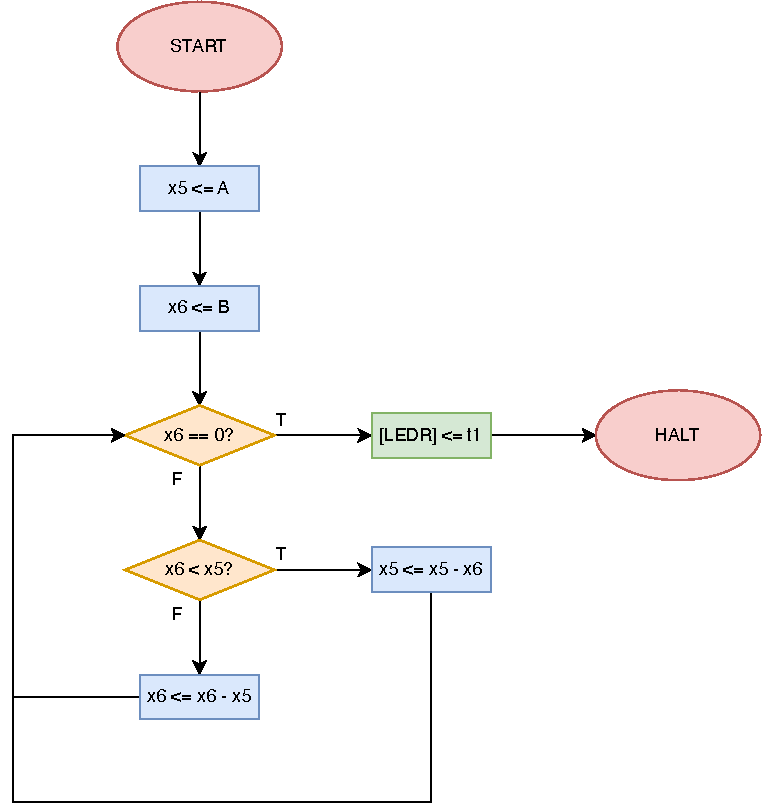
\includegraphics[width=.75\textwidth]{images/flowchart/gcd.pdf}
    \caption{Program flow for GCD Calculation}
\end{figure}

Below are the input of $A$ and $B$ are set in DMEM, at the end of the program, the result will be shown on the LEDR. This program utilized \texttt{sub}, \texttt{lw}, \texttt{sw}, \texttt{beq}, \texttt{blt}, \texttt{jal} and \texttt{auipc} instructions.

\begin{minted}{text}
A = 48, B = 18, LEDR = 6
A = 92, B = 254, LEDR = 2
A = 68, B = 119, LEDR = 17
\end{minted}

\chapter{FPGA Implementation}
\section{Show the \nth{46} element of the Fibonacci Sequence}
The \nth{46} element of the Fibonacci sequence is obtained using the test program from the section \ref{fibonacci}, and the resulting value is displayed on the LEDR in binary form. Instructions for storing the value into BIN2BCD are added to convert it into a BCD format, and then it is stored directly in the HEX2HEX component to be shown on the 7-segment displays.

Due to the number's 10-digit length, only 8 of the 7-segment displays are utilized, resulting in the omission of the 2 most significant digits from the display.

\begin{figure}[H]
    \centering
    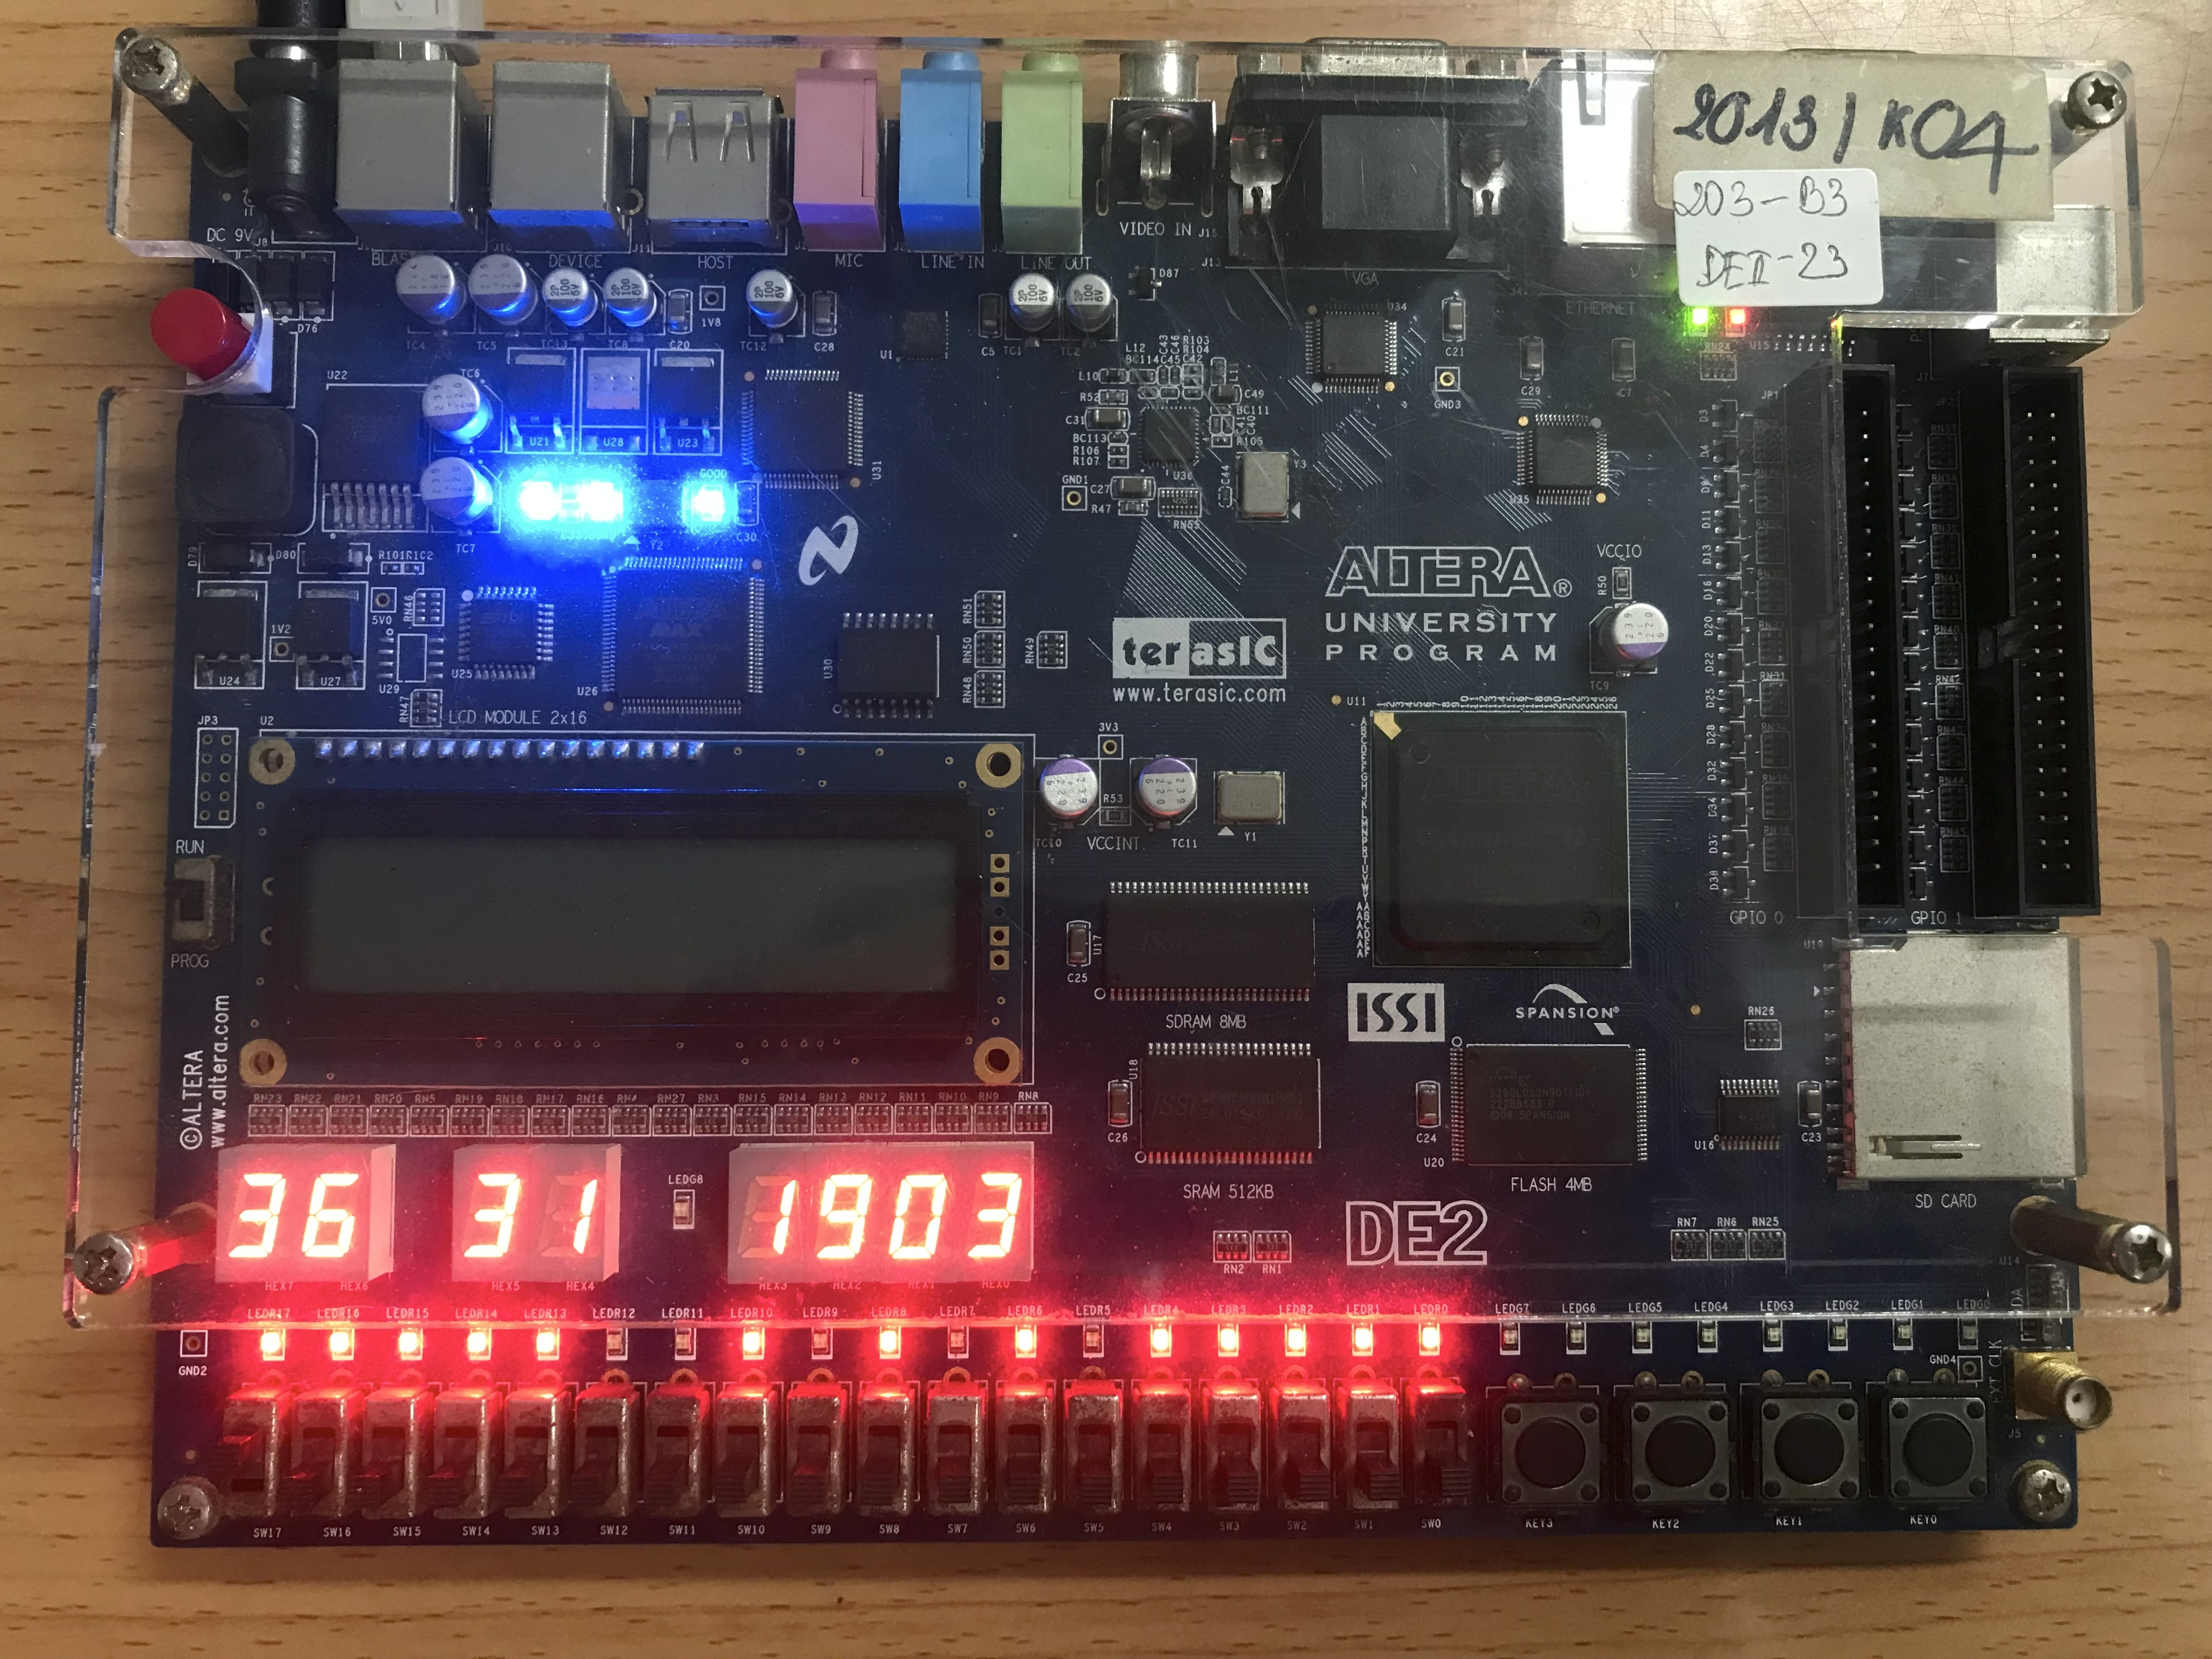
\includegraphics[width=.8\textwidth]{images/fibonacci_fpga.jpg}
    \caption{\nth{46} number of the Fibonacci sequence shown on the 7-segment displays}
\end{figure}

\section{Stopwatch}

\begin{figure}[H]
    \centering
    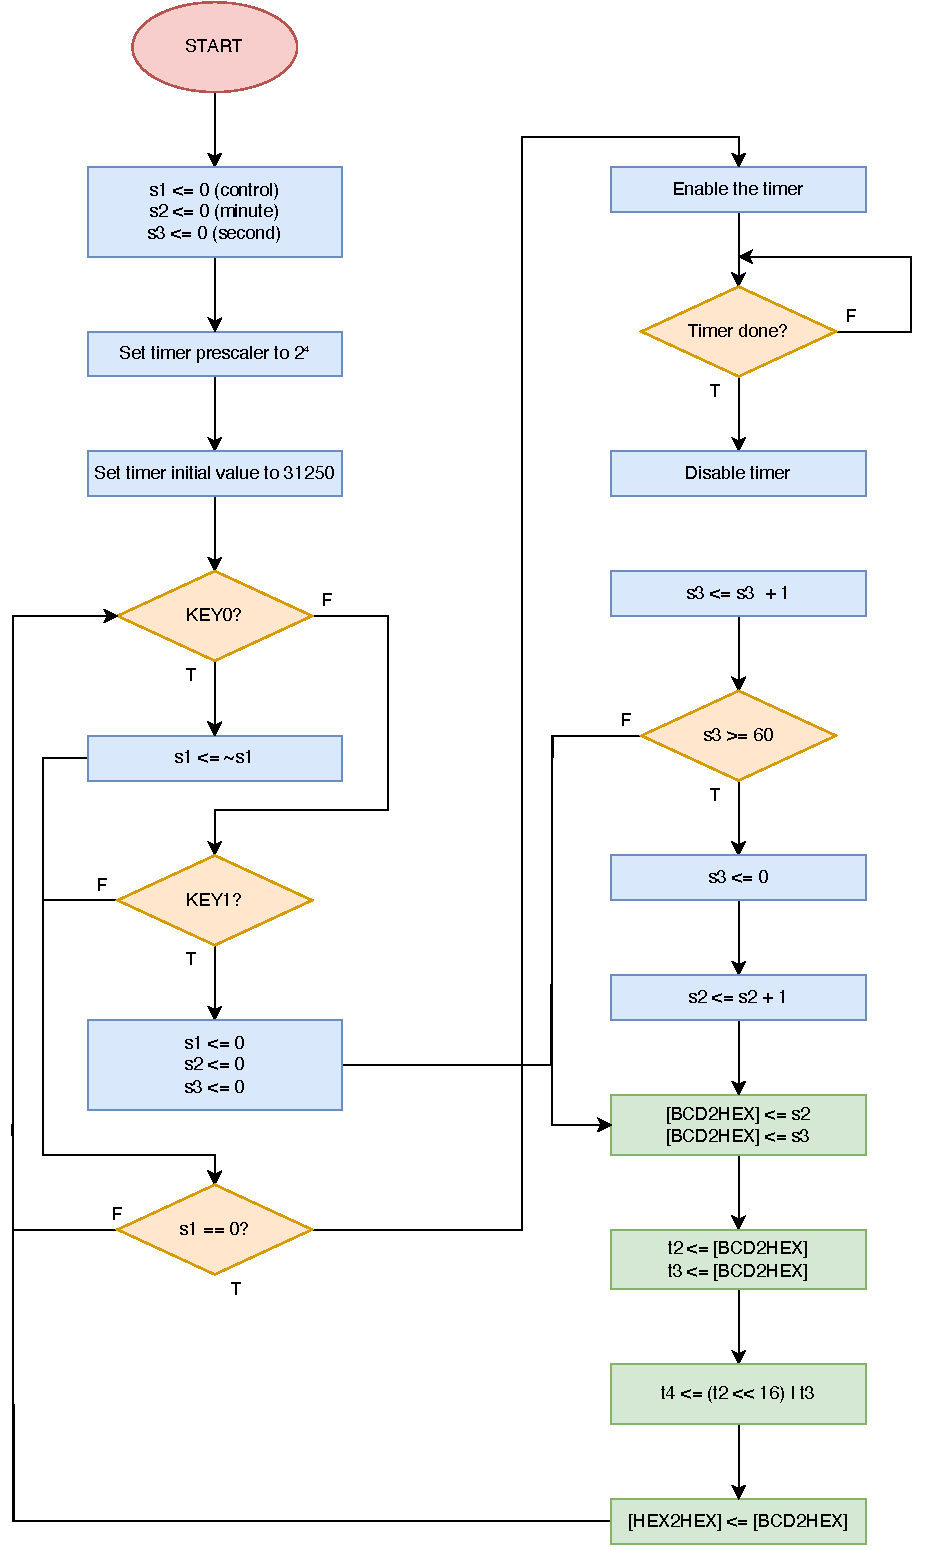
\includegraphics[width=.7\textwidth]{images/flowchart/stopwatch.pdf}
    \caption{Program flow for stopwatch}
\end{figure}

The program starts by initializing register \texttt{s3} to 0, which will be used to store the timer value. It then configures the timer by setting the prescaler to $2^4$ (a division by 16), and the initial timer value to 31250. After enabling the timer, with the CPU running at \texttt{50MHz}, the timer will trigger the \texttt{done} signal after 10 milliseconds (0.01 seconds). Once the timer is done, it is disabled, and the program increments the \texttt{s3} register. The value stored in \texttt{s3} is then converted to BCD using the \texttt{BIN2BCD} module. This BCD value is further store to \texttt{HEX2HEX} for displaying it on 8 7-segment displays. The program would continue to loop.

When the reset is de-asserted (\texttt{SW17} = 1), the seven segment is reset to \texttt{00 00 0000}.

 \begin{figure}[H]
    \begin{center}
    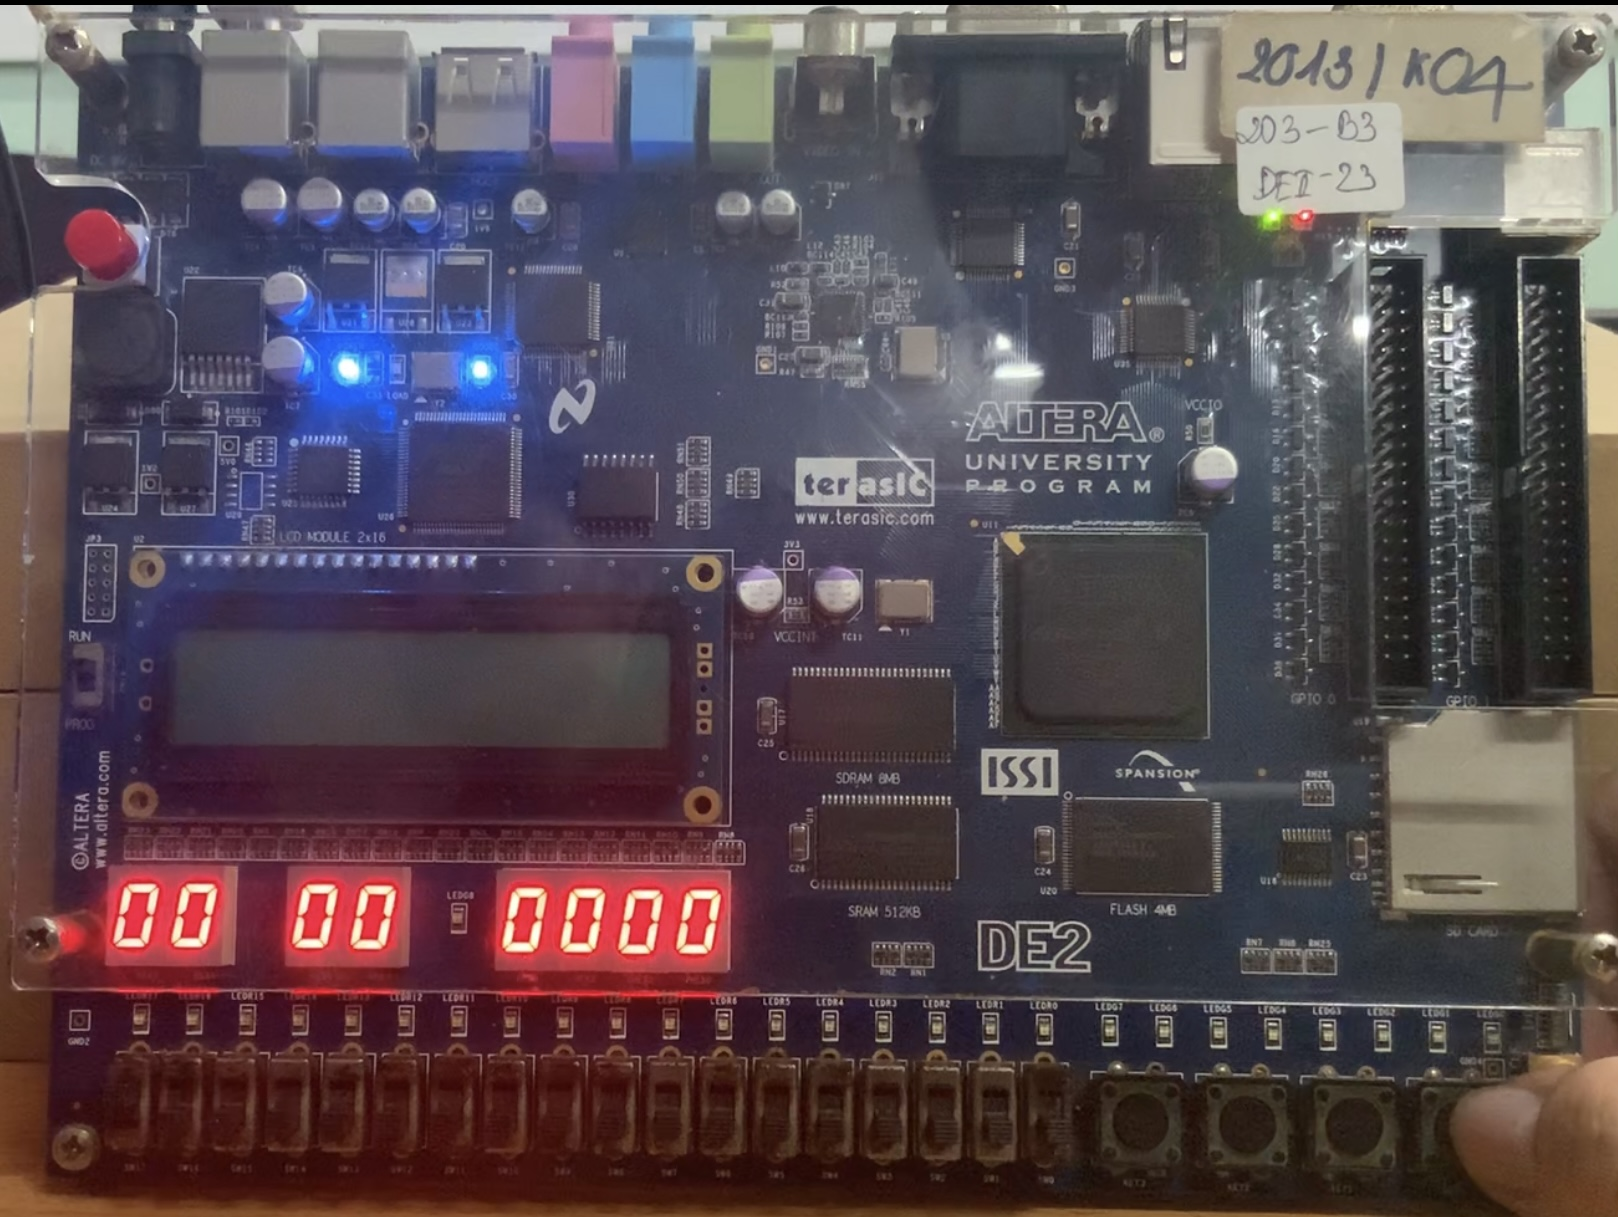
\includegraphics[width=.82\textwidth]{images/timer1.jpg}
    \caption{The initial state of stop watch timer}
    \end{center}
\end{figure}

After pressing the \texttt{KEY0}, the stopwatch begin to count, then the timer will be displayed on the seven-segment displays. Pressing the \texttt{KEY0} again would pause the stopwatch, the image below showing the stopwatch is paused at (\texttt{00 00 0135}), which means 1.35s.

 \begin{figure}[H]
    \begin{center}
    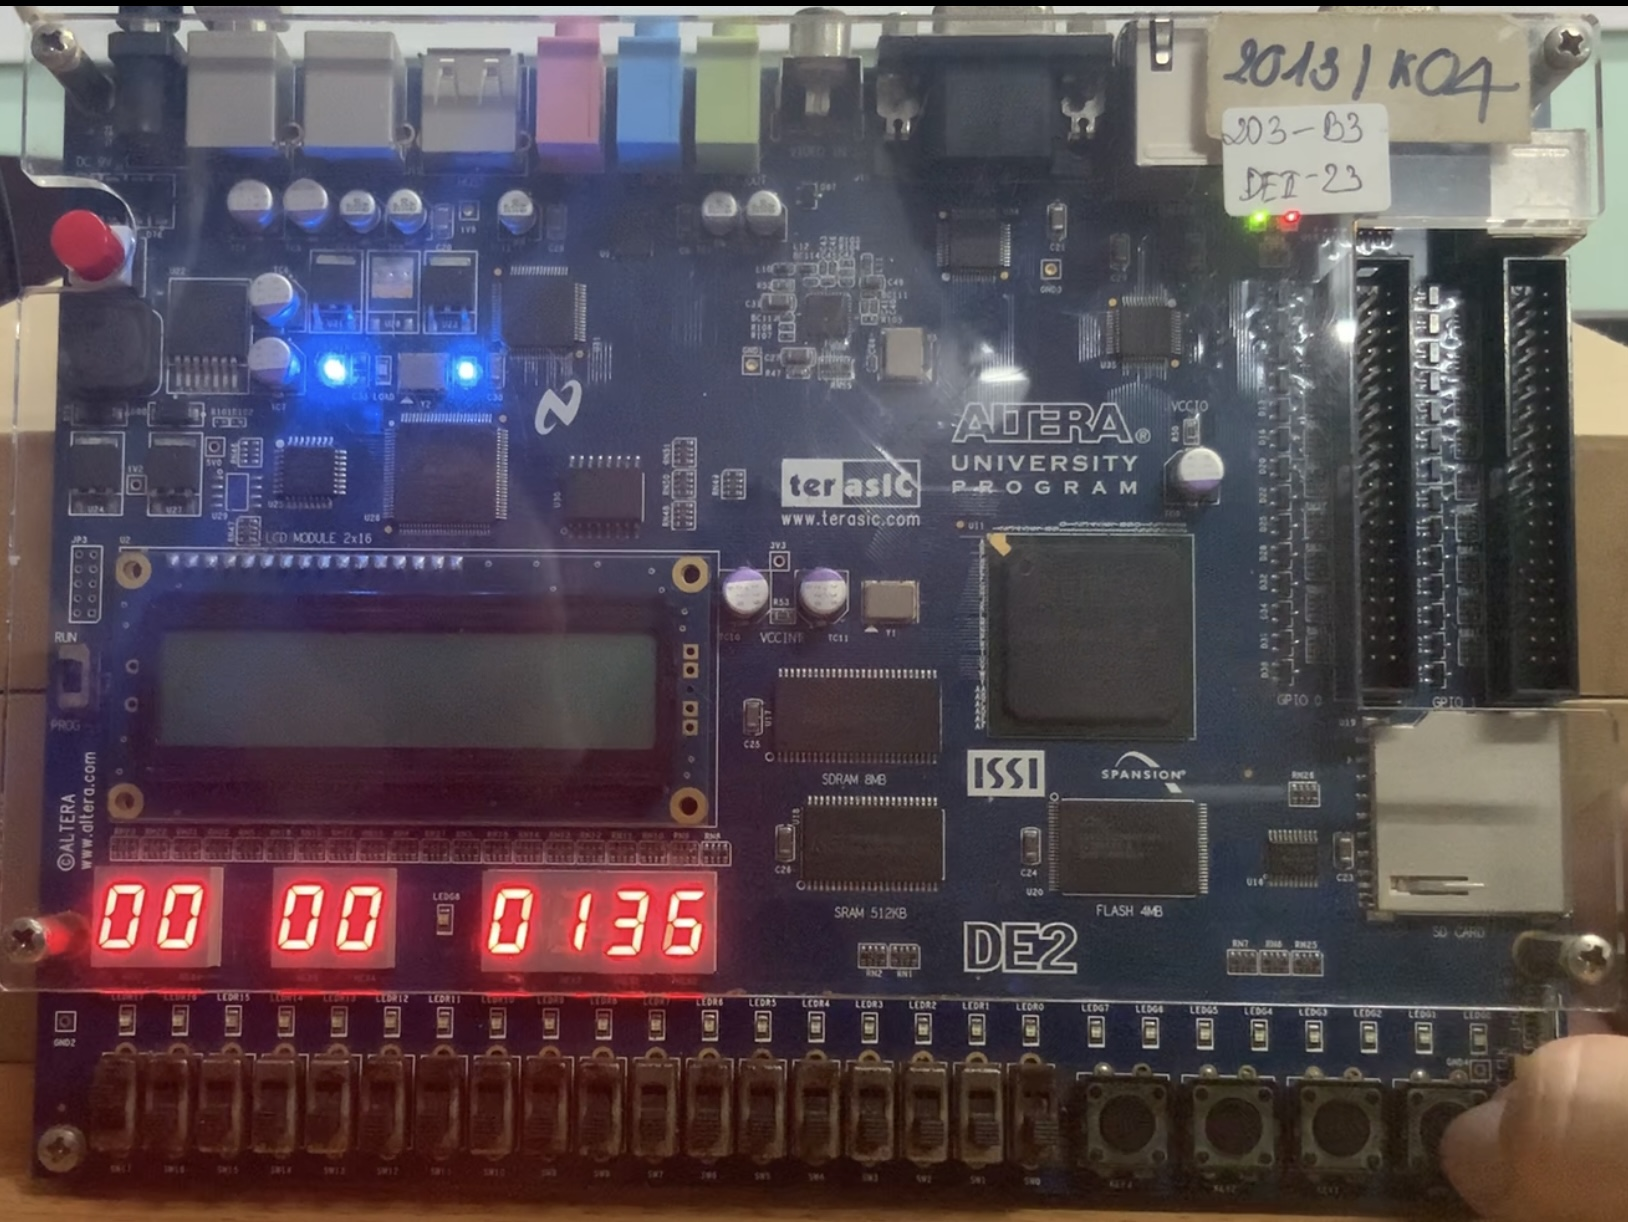
\includegraphics[width=.82\textwidth]{images/timer2.jpg}
    \caption{The stopwatch timer displaying on HEX at 1.35s}
    \end{center}
\end{figure}

Pressing the \texttt{KEY1} would reset the stopwatch to 0.

 \begin{figure}[H]
    \begin{center}
    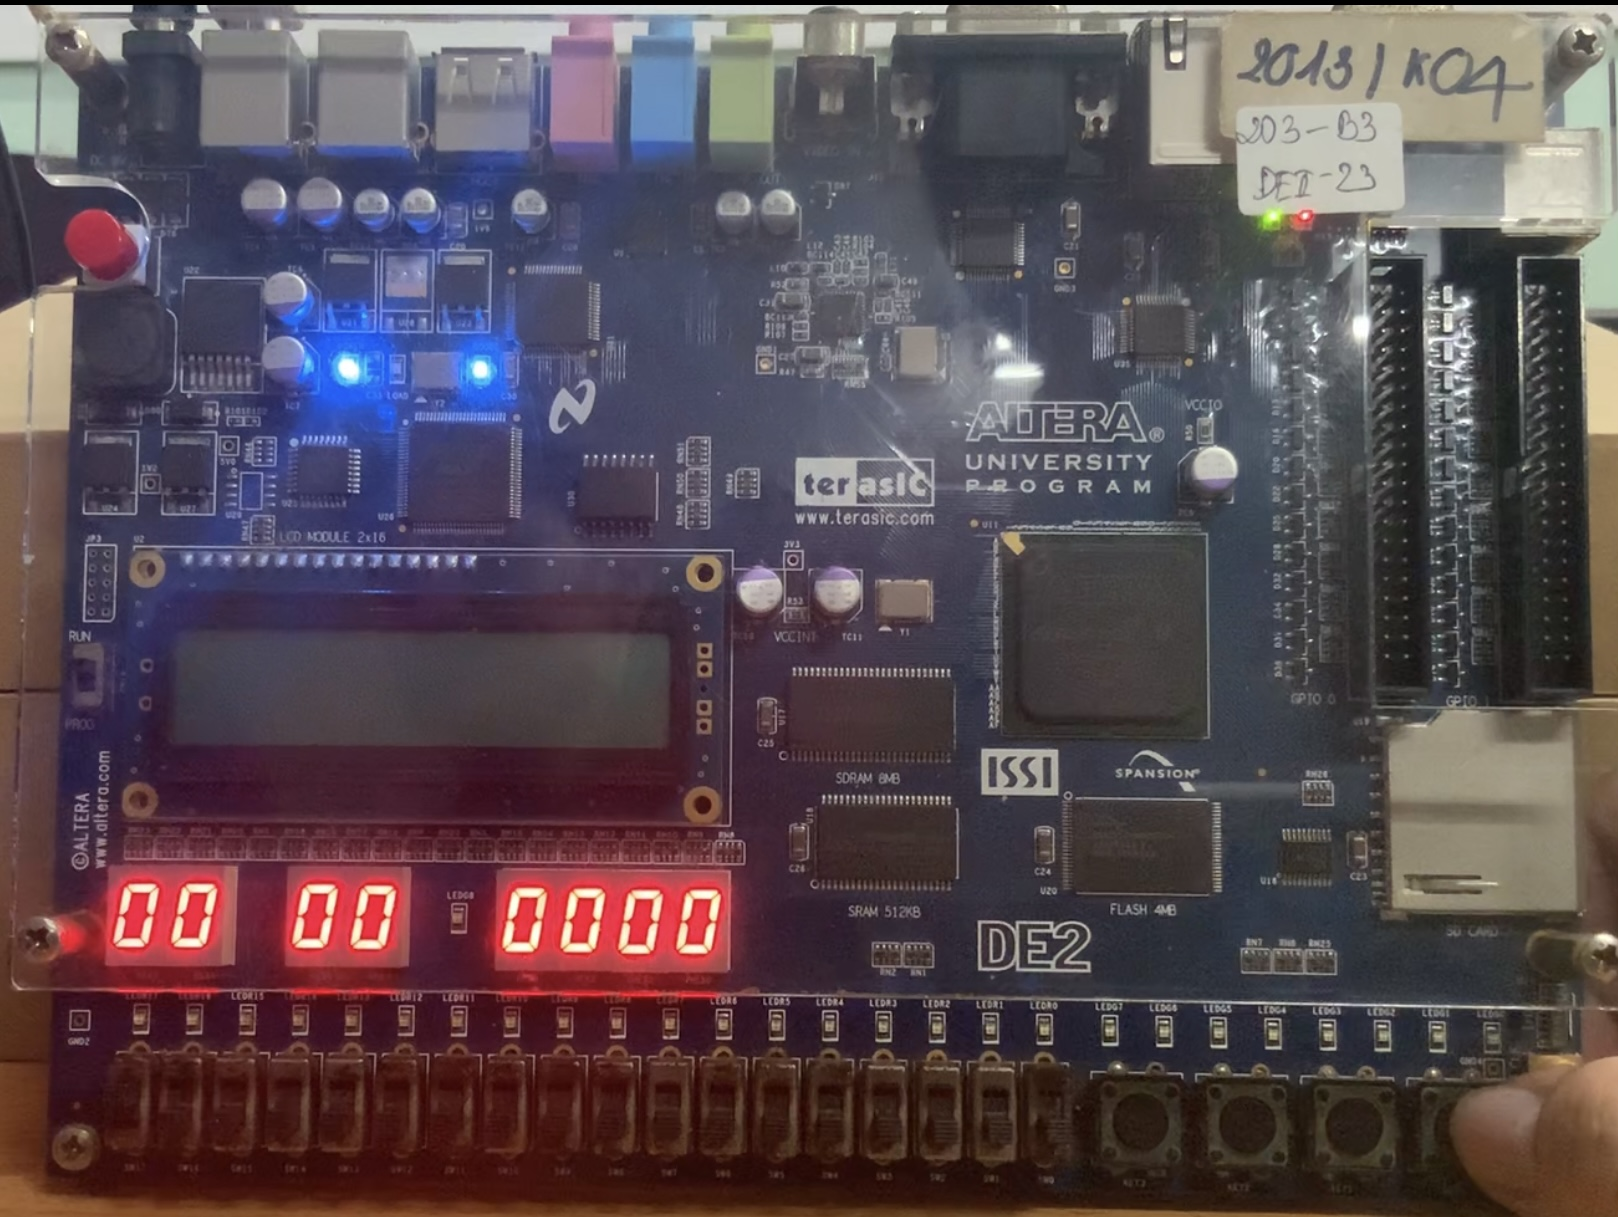
\includegraphics[width=.80\textwidth]{images/timer1.jpg}
    \caption{The stop watch timer after pressing the \texttt{KEY1}}
    \end{center}
\end{figure}

The image below displays the stopwatch being captured at the transition from \texttt{17:52.31} to \texttt{17:52.32}.

 \begin{figure}[H]
    \begin{center}
    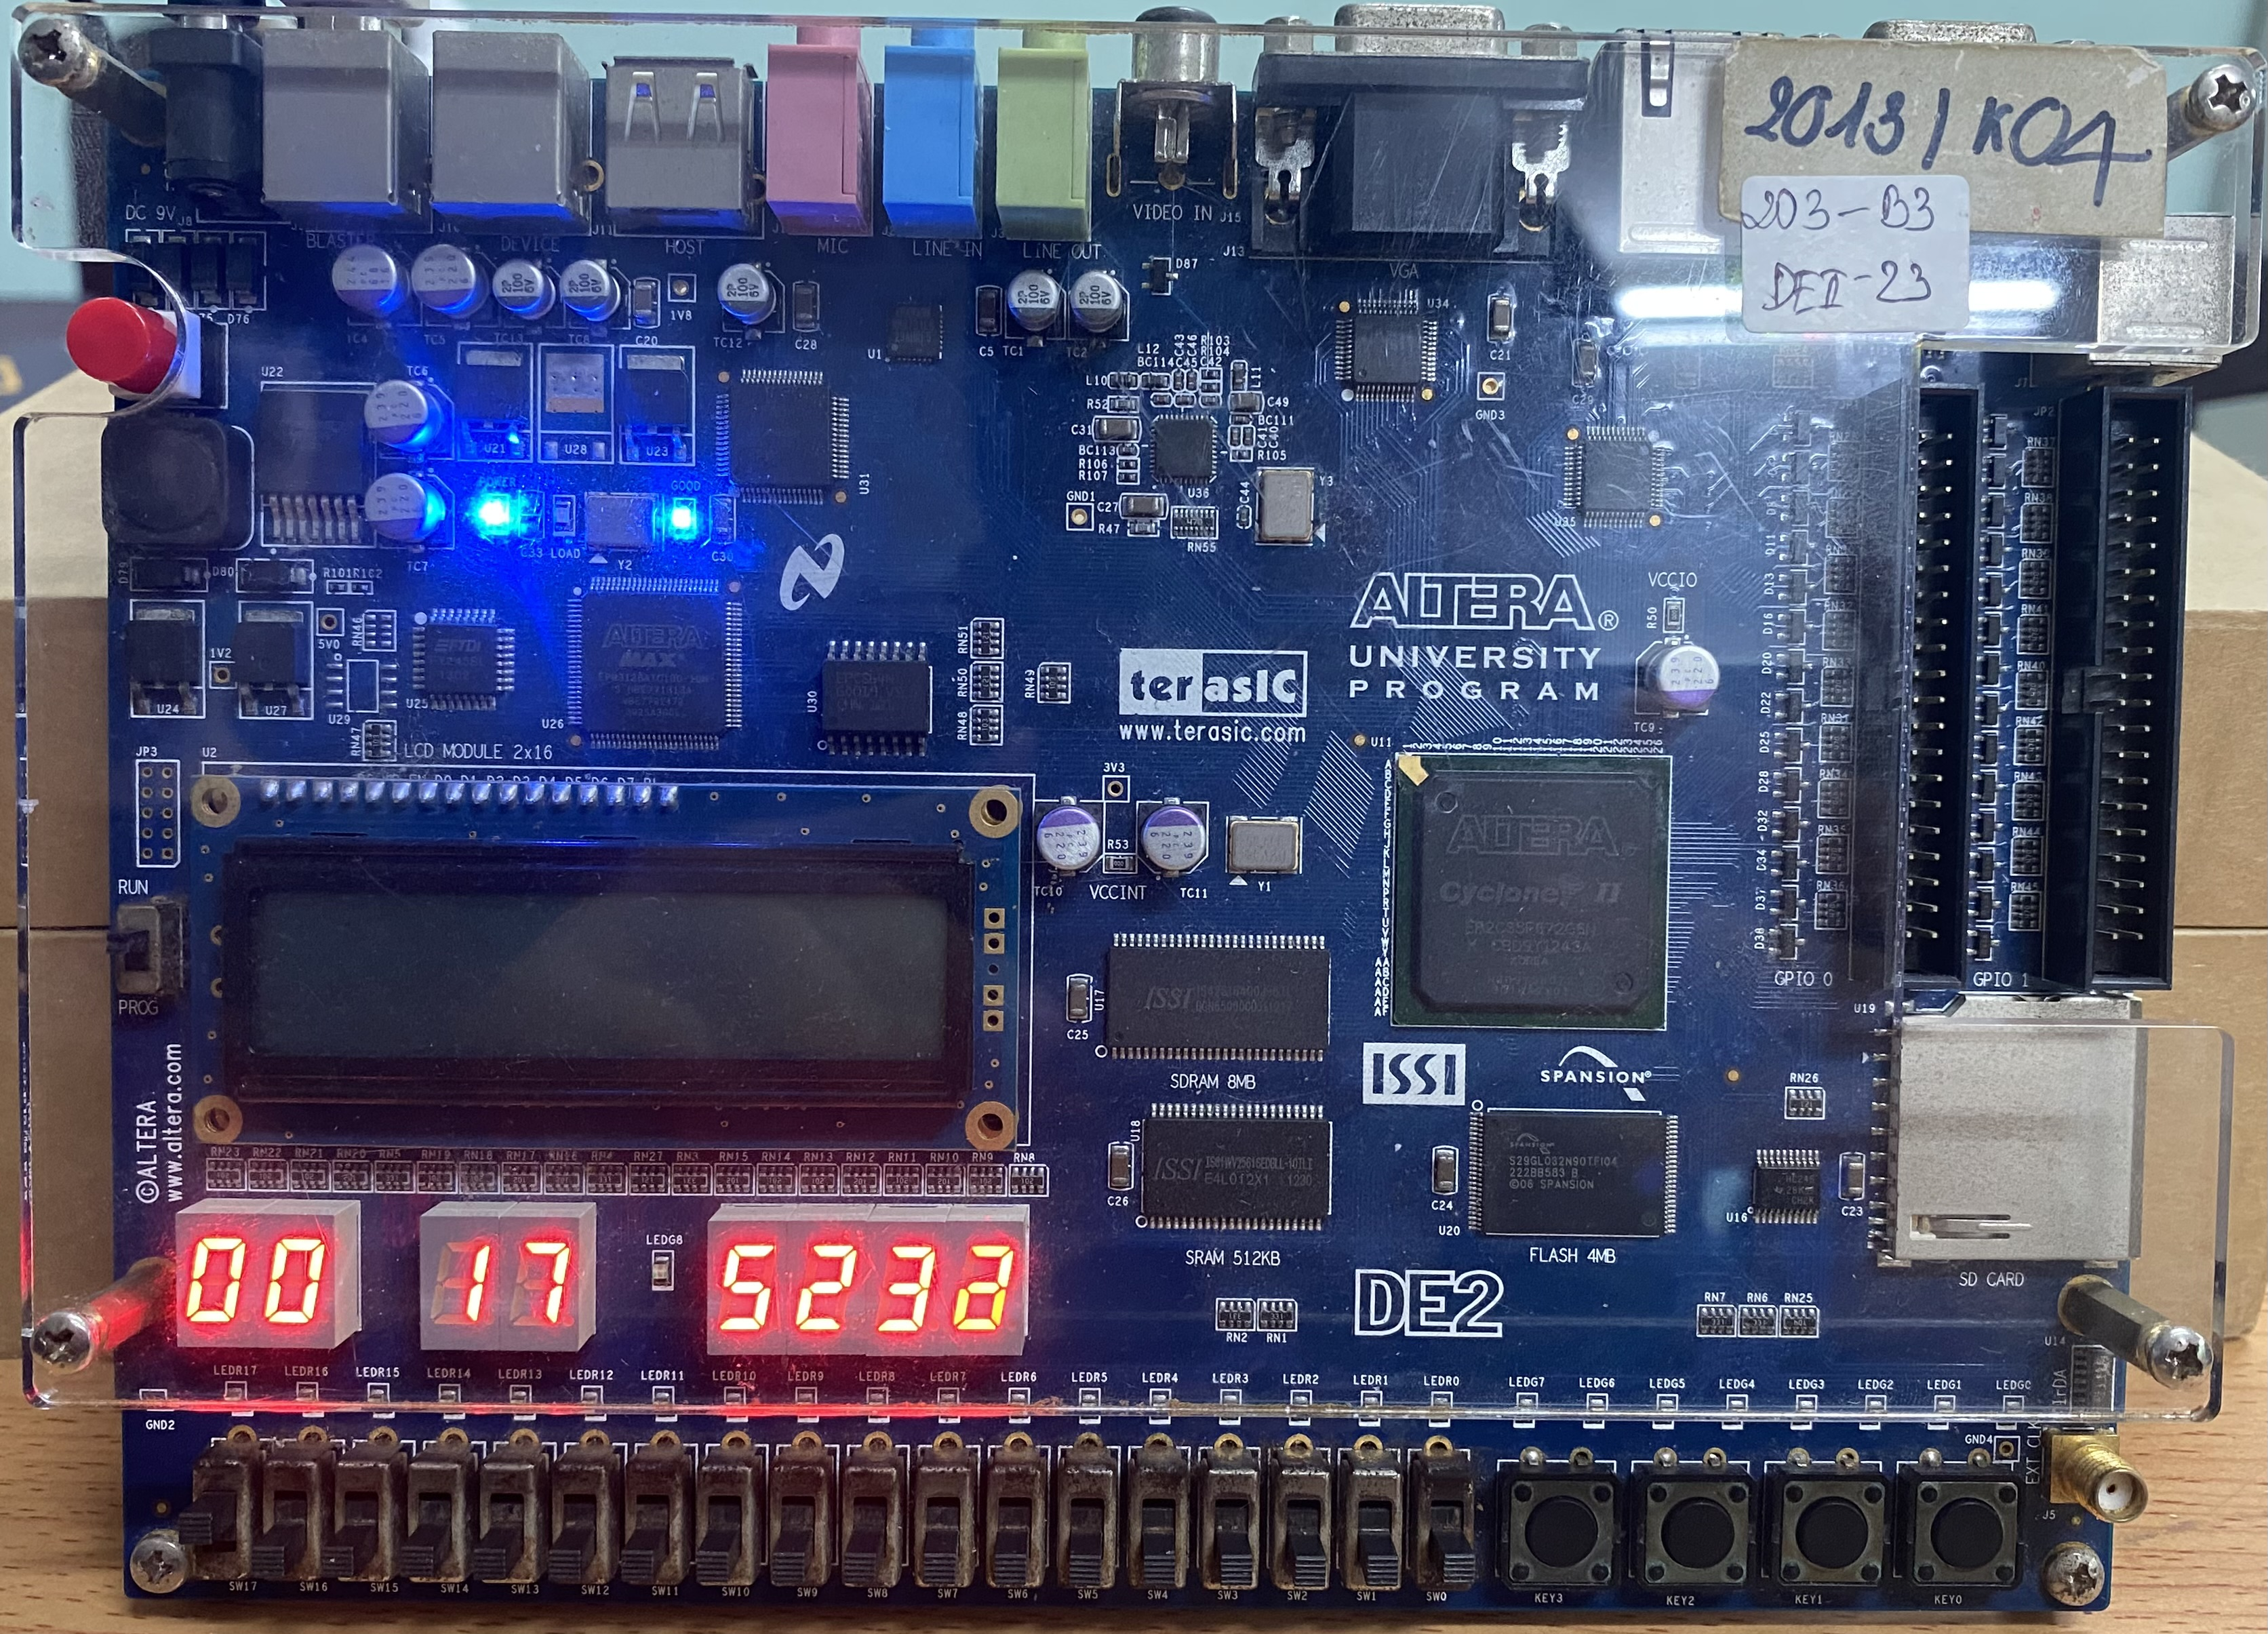
\includegraphics[width=.80\textwidth]{images/timer3.jpg}
    \caption{The stop watch timer displaying on HEX at 17m52.32s}
    \end{center}
\end{figure}

A seven-minute demonstration of the stopwatch functionality is available at \url{https://youtu.be/uoGHKLeUYAw}

\section{Display \texttt{Hello!} on the LCD}
\begin{figure}[H]
    \centering
    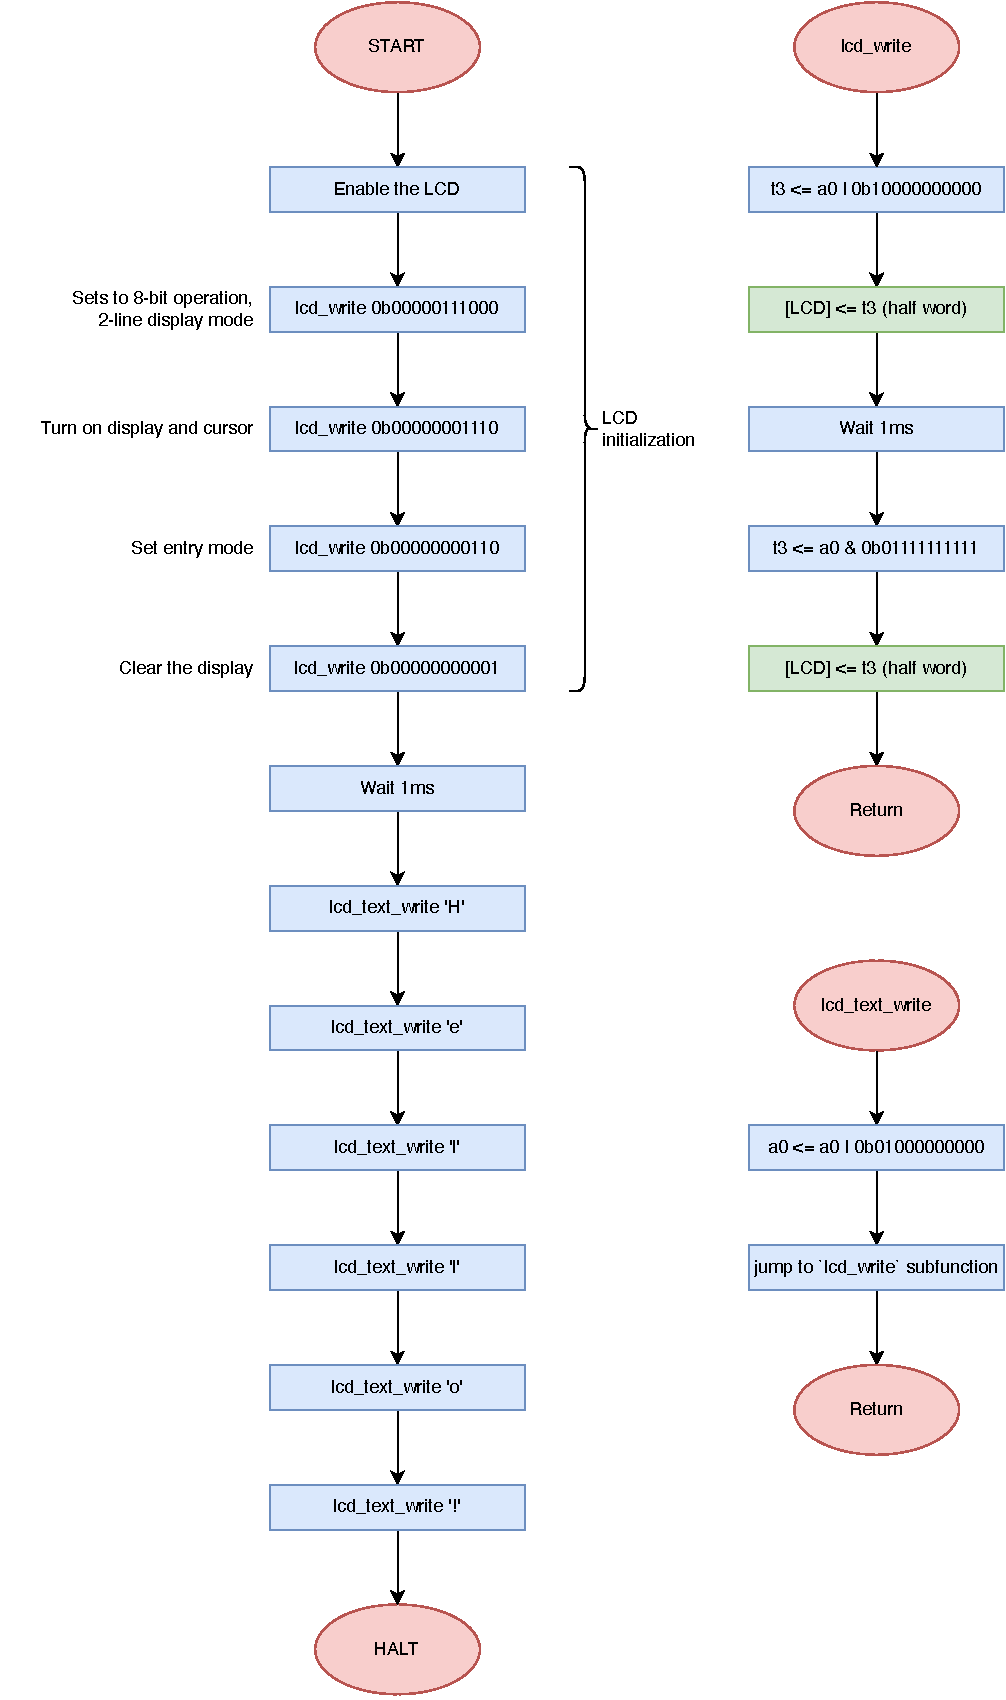
\includegraphics[width=.8\textwidth]{images/flowchart/lcd.pdf}
    \caption{Program flow for LCD writing}
\end{figure}

\begin{figure}[H]
    \centering
    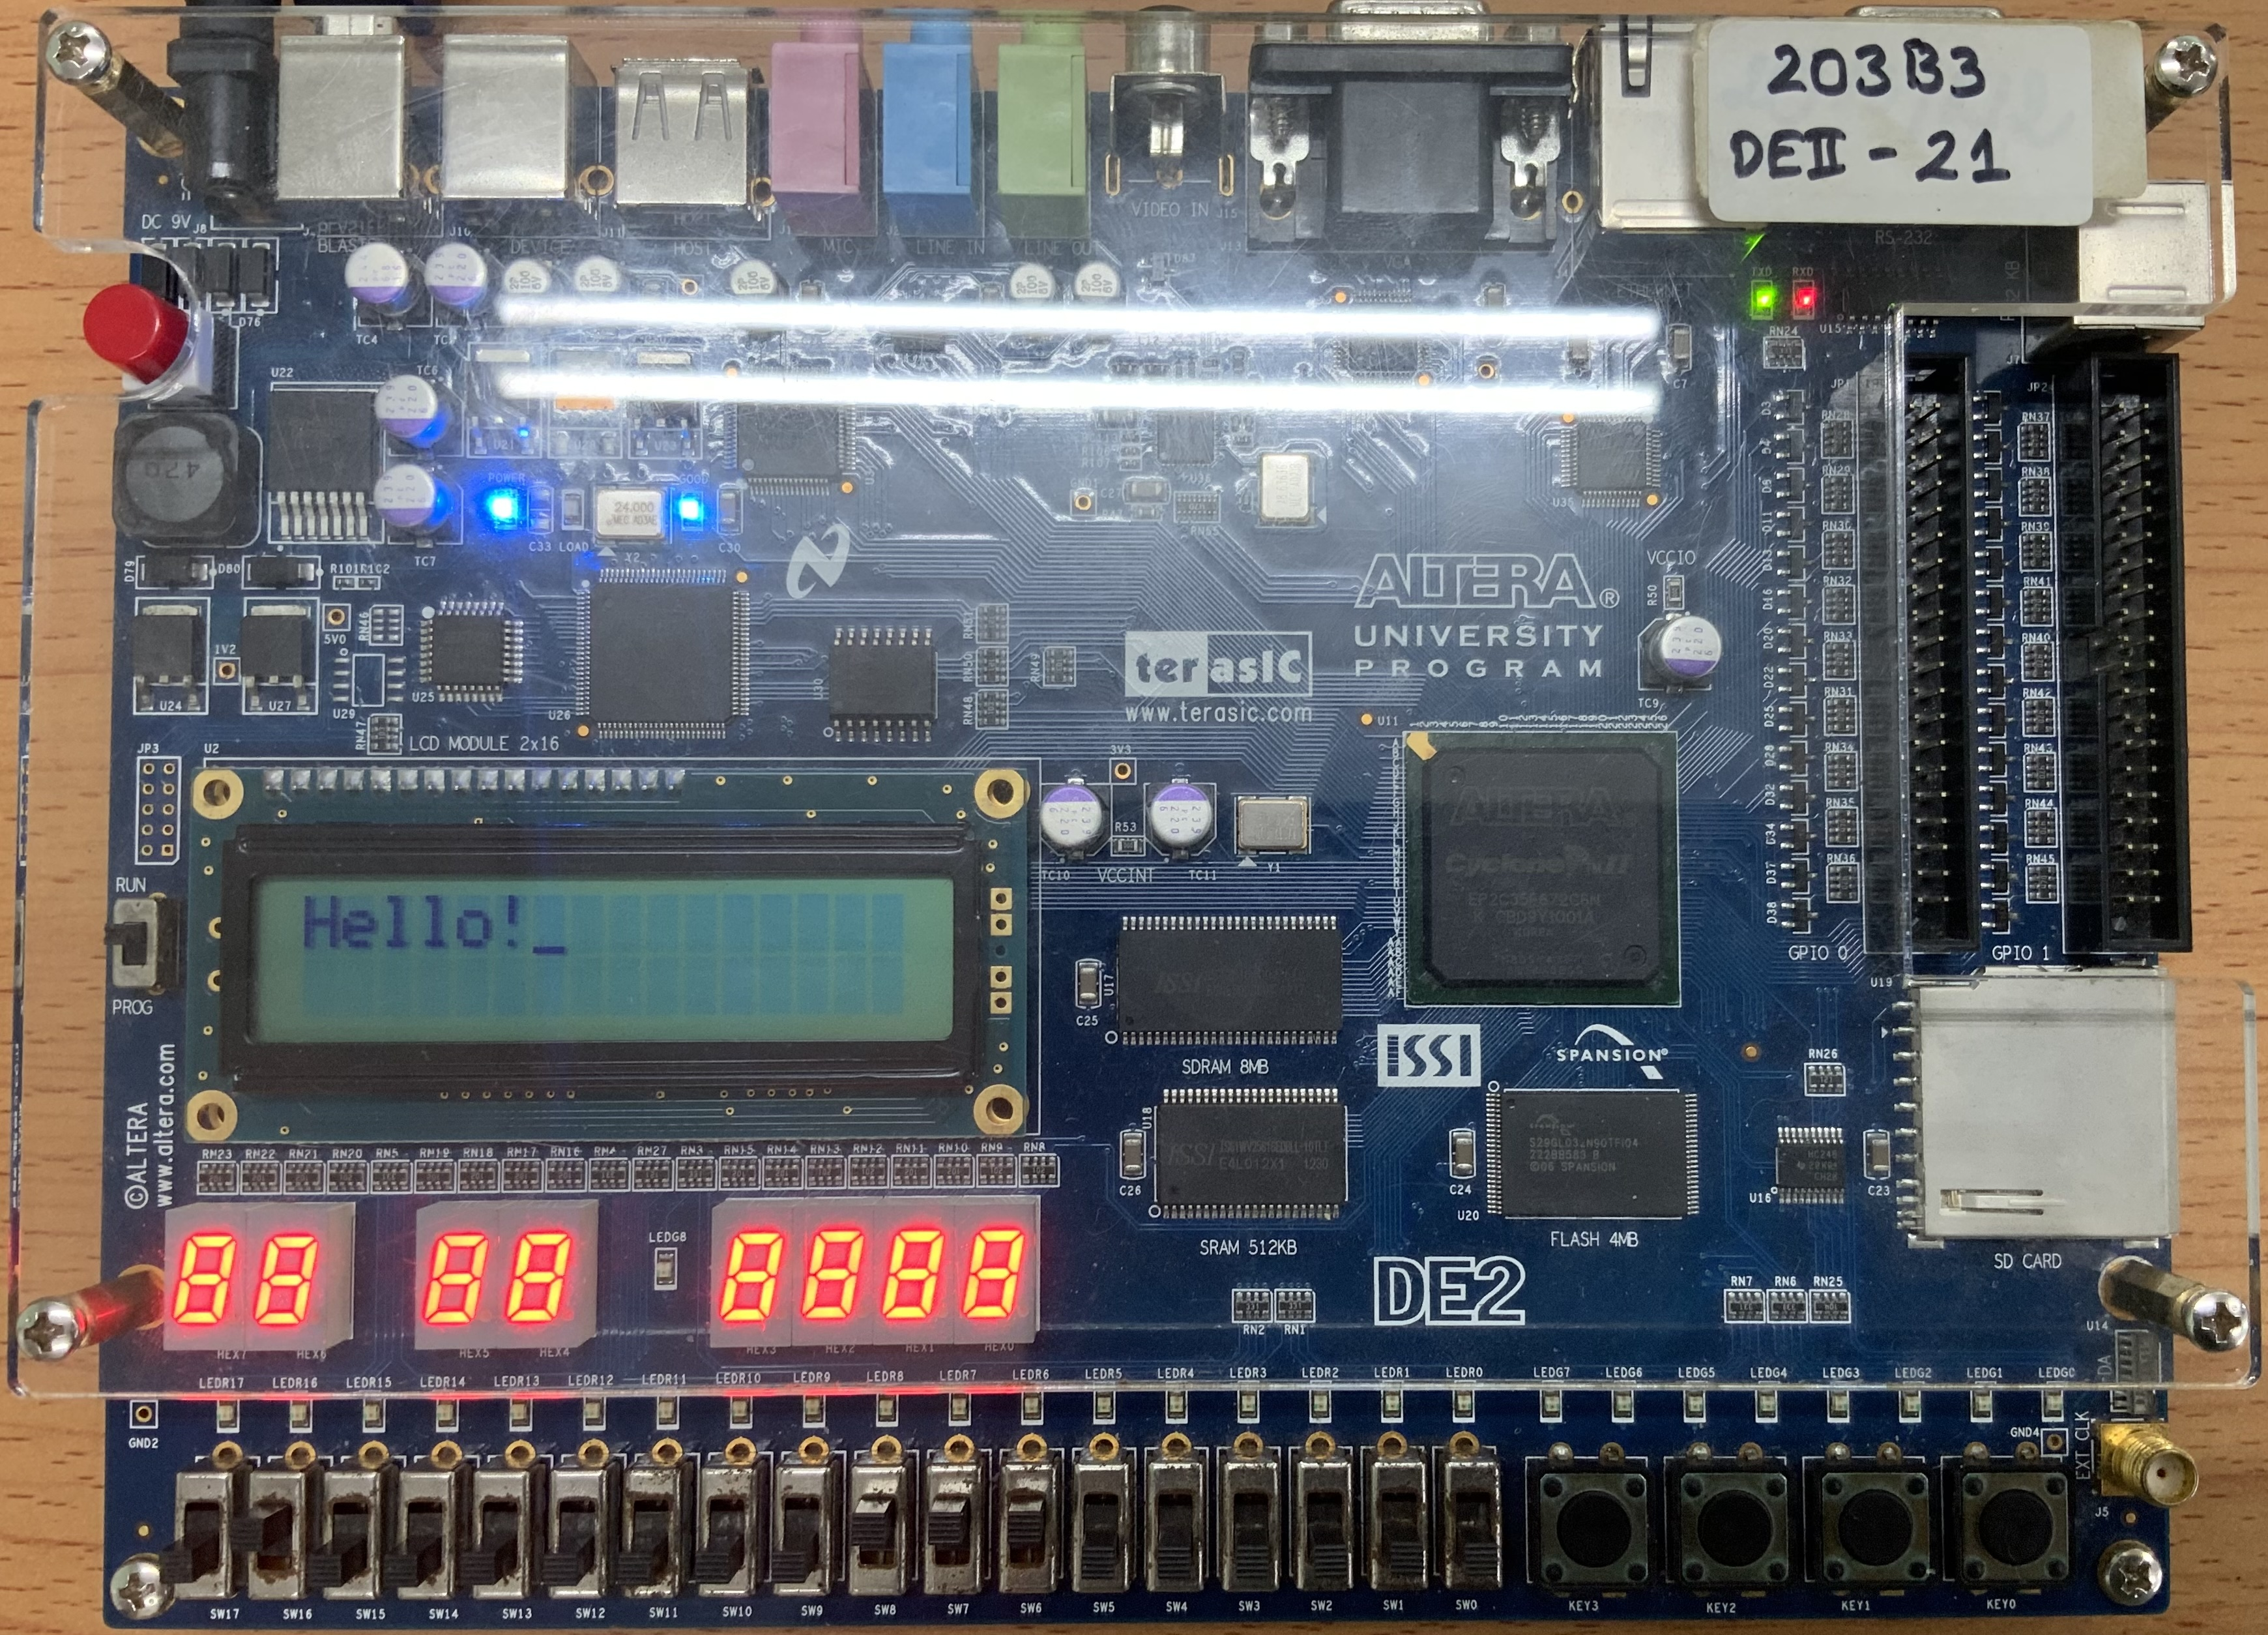
\includegraphics[width=.80\textwidth]{images/hello.jpg}
    \caption{\texttt{Hello!} text on the LCD}
\end{figure}

\begin{figure}[H]
    \centering
    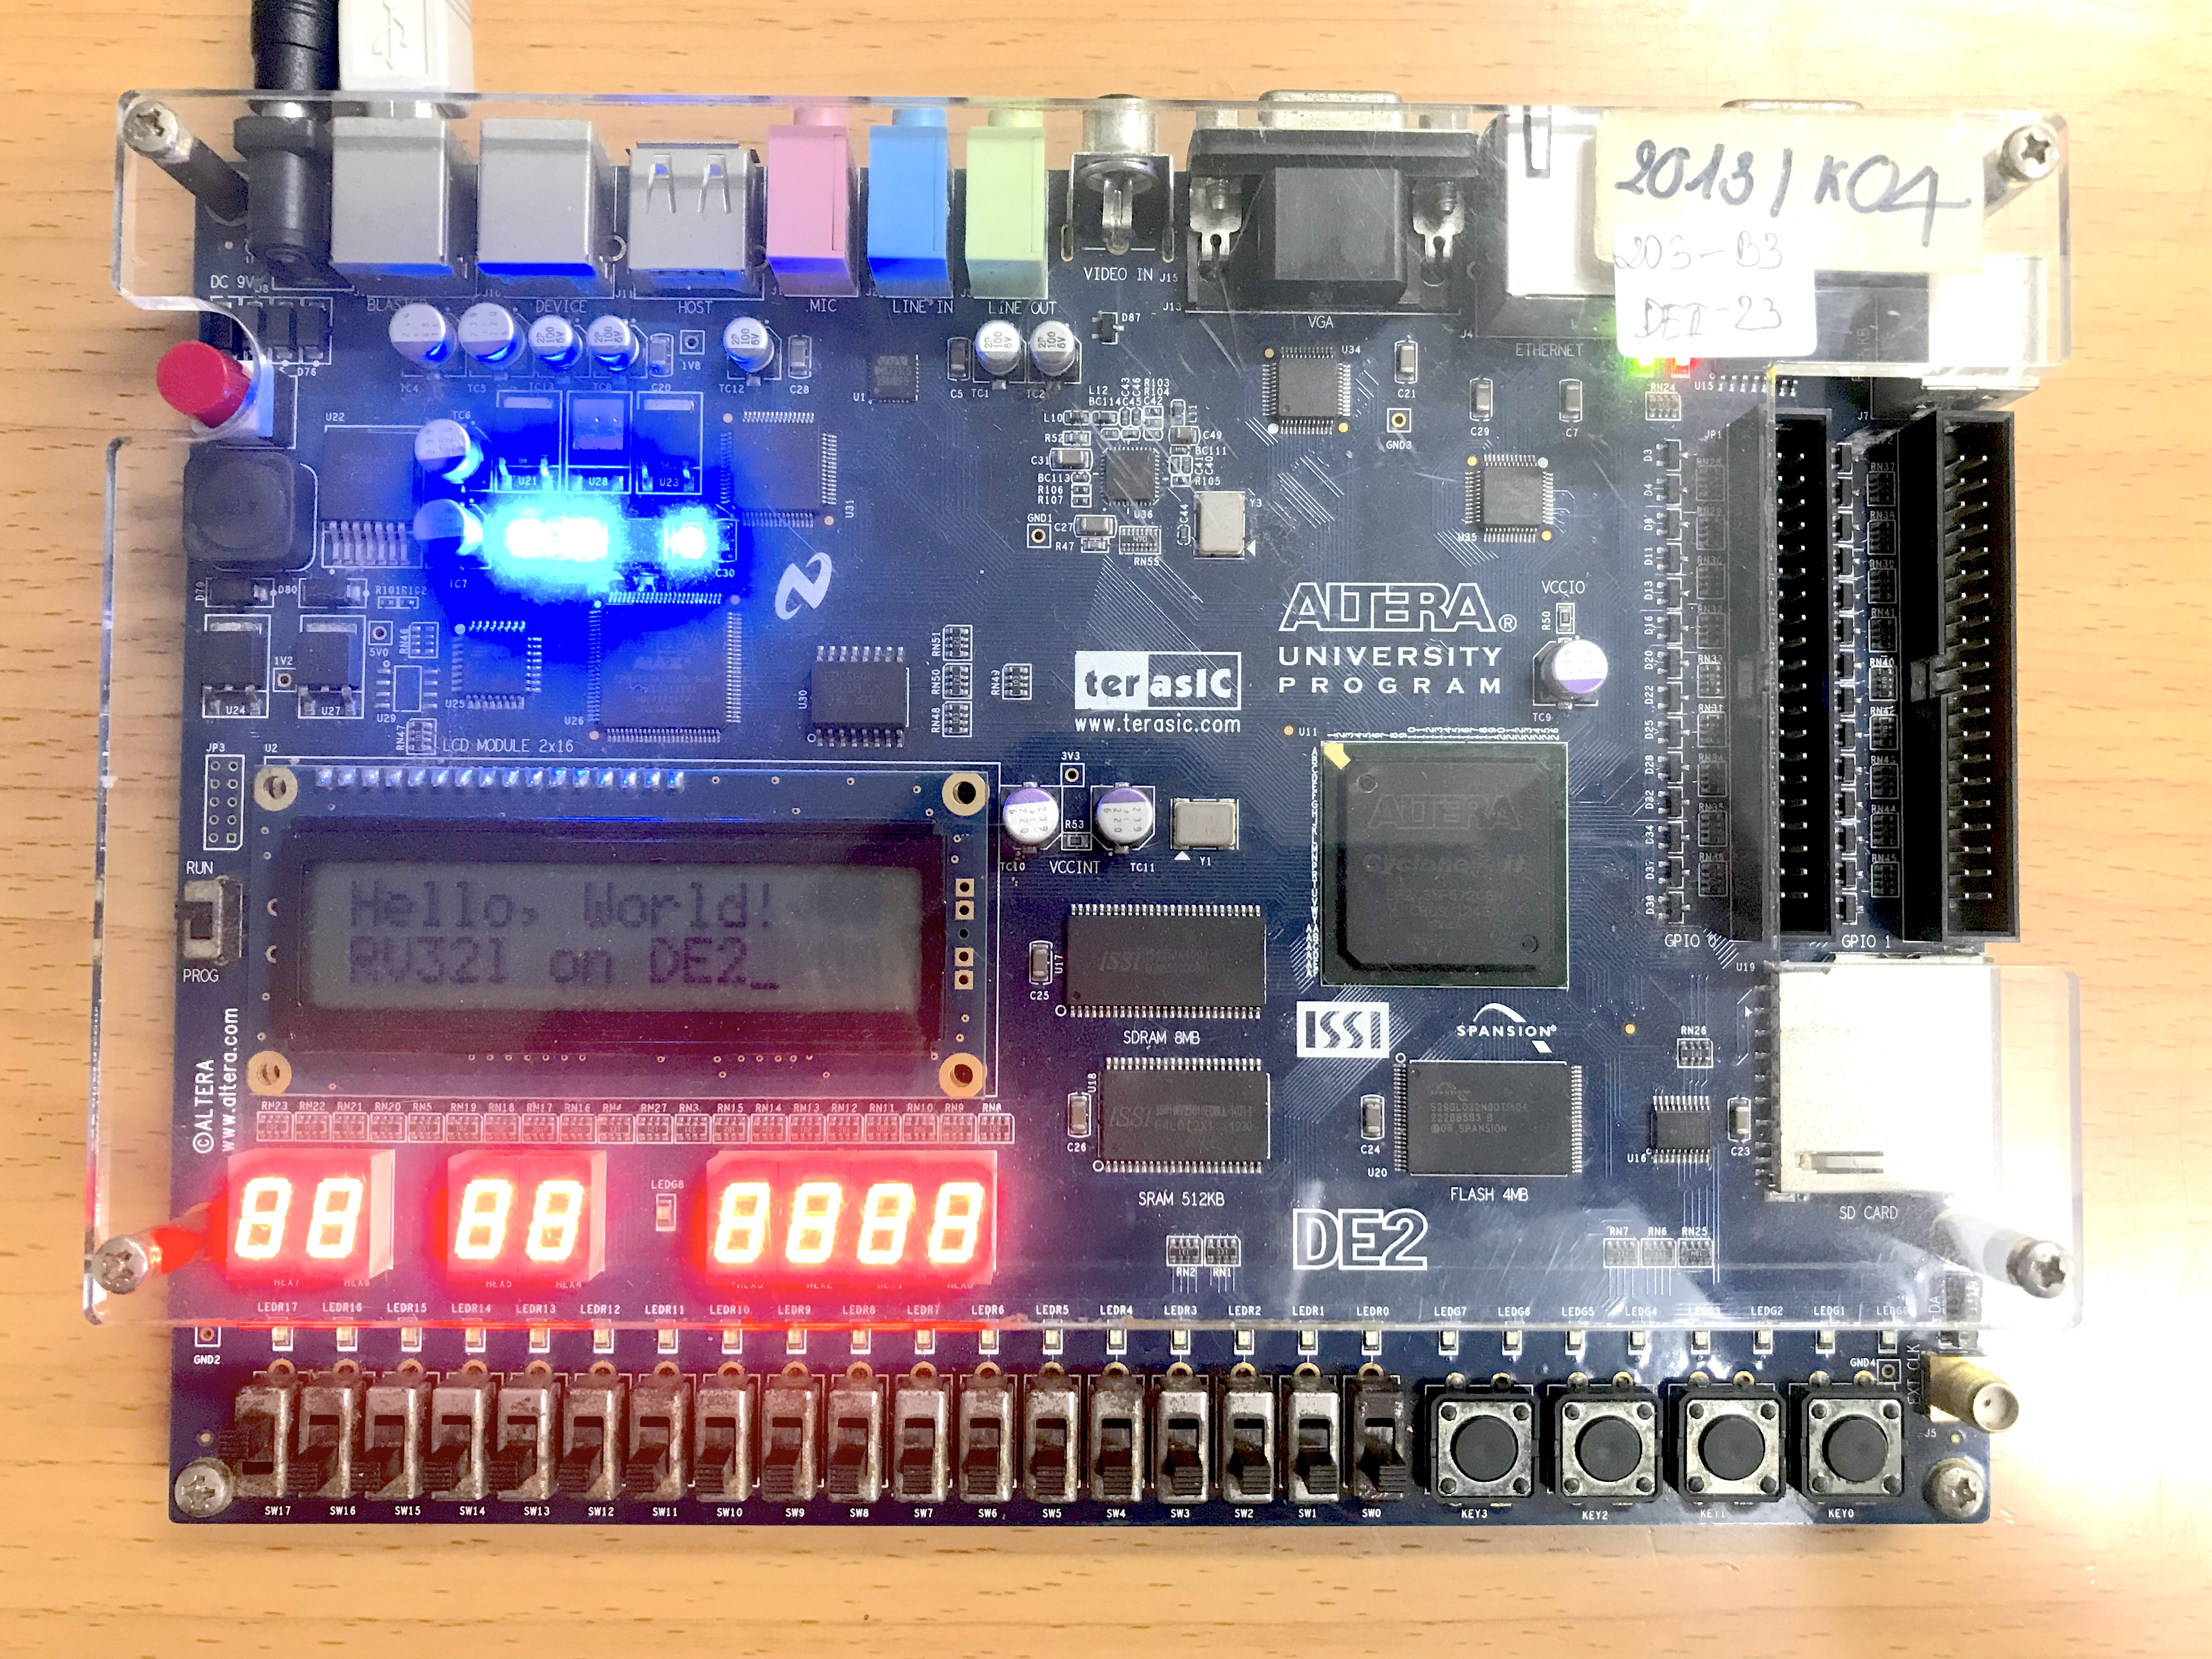
\includegraphics[width=.80\textwidth]{images/helloworld.jpg}
    \caption{$
    \begin{array}{l}
        \texttt{Hello, World!}\\
        \texttt{RV32I on DE2}
    \end{array}
    $ text on the LCD}
\end{figure}

\section{Input coordinates of A, B and C. Display the point is closer to C}
In this application, the user interacts with the program by inputting three coordinates for points A, B, and C using SWs. The selection of the number is facilitated by the toggling SWs, where the maximum input value is limited to 99. The value is directly displayed on the 7-segment displays. After toggling the switch, pressing any key serves as the enter button to confirm the input. Once the coordinates for all three points are provided, the program proceeds to calculate the distances between points A and C, as well as B and C. The program then determines which point has the smaller distance, and the result is displayed on the LCD. In the case where the distances are equal, both points A and B are printed.

In this application program, the objective is to calculate the power of the difference between two sets of coordinates represented by variables $x$ and $y$. To achieve this, sub-functions for absolute value (\texttt{abs}) and power (\texttt{pow}) have been designed. The flow diagrams for these sub-functions are depicted below. 

\begin{figure}[H]
    \centering
    \includegraphics[width=.9\textwidth]{images/flowchart/pow_abs.pdf}
    \caption{\texttt{pow} and \texttt{abs} sub-program}
\end{figure}

\begin{figure}[H]
    \centering
    \includegraphics[width=.5\textwidth]{images/flowchart/app4.pdf}
    \caption{Program flow for the applicaiton 4}
\end{figure}

Set the $x$-coordinate of $A$ is 3, and the $y$-coordinate of $A$ is 4. 

 \begin{figure}[H]
    \begin{center}
    \includegraphics[width=.85\textwidth]{images/applicationA.jpg}
    \caption{Set input for point A(3,4)}
    \end{center}
\end{figure}

Set the $x$-coordinate of $B$ is 5, and the $y$-coordinate of $B$ is 1. 
 \begin{figure}[H]
    \begin{center}
    \includegraphics[width=.85\textwidth]{images/applicationB.jpg}
    \caption{Set input for point B(5,1)}
    \end{center}
\end{figure}

Set the $x$-coordinate of $C$ is 0, and the $y$-coordinate of $C$ is 0. 
 \begin{figure}[H]
    \begin{center}
    \includegraphics[width=.8\textwidth]{images/application.jpg}
    \caption{Set input for point C(0,0) and display the result}
    \end{center}
\end{figure}
We know that $d_{AC} = \sqrt{3^2 + 4^2} = 5$, $d_{BC} = \sqrt{5^2 + 1^2} = \sqrt{26} \approx 5,0991$, so point $A$ closer to $C$. After pressing the \texttt{KEY0}, the LCD would display \texttt{A}.

 \begin{figure}[H]
    \begin{center}
    \includegraphics[width=.8\textwidth]{images/timer6.jpg}
    \caption{Result for $A(99,15)$, $B(3,3)$, $C(1,1)$}
    \end{center}
\end{figure}
We know that $d_{AC} = \sqrt{98^2 + 14^2} = 70 \sqrt{2}$, $d_{BC} = \sqrt{2^2 + 2^2} = 2 \sqrt{2}$, so point $B$ closer to $C$. After pressing the \texttt{KEY0}, the LCD would display \texttt{B}.

% \chapter{Alternative Design}
 \begin{figure}[H]
    \begin{center}
    \includegraphics[width=.8\textwidth]{images/timer4.jpg}
    \caption{Result for $A(4,0)$, $B(6,0)$, $C(5,0)$}
    \end{center}
\end{figure}
We know that $d_{AC} = \sqrt{1^2 + 0^2} = 1$, $d_{BC} = \sqrt{1^2 + 0^2} = 1$, so both point $A$ and $B$ closer to $C$. After pressing the \texttt{KEY0}, the LCD would display \texttt{AB}.

 \begin{figure}[H]
    \begin{center}
    \includegraphics[width=.8\textwidth]{images/timer5.jpg}
    \caption{Result for $A(0,1)$, $B(0,1)$, $C(0,1)$}
    \end{center}
\end{figure}
We know that $d_{AC} = \sqrt{0^2 + 0^2} = 0$, $d_{BC} = \sqrt{0^2 + 0^2} = 0$, so both point $A$ and $B$ closer to $C$. After pressing the \texttt{KEY0}, the LCD would display \texttt{AB}.

The entire procedural demonstration is available at \url{https://youtu.be/vPrqrwcz0Q8}.

\chapter{Evaluation}

\begin{table}[H]
\caption{Evaluation of the tasks}
\begin{flushright}
\small$\times$ bad ; -- uncomment ; \checkmark good
\end{flushright}

\resizebox{.97\columnwidth}{!}{%
\begin{tabular}{|c|l|c|}
\hline
\multicolumn{2}{|c|}{\textbf{Tasks}} & \textbf{Evaluation} \\ \hline
\multirow{14}{*}{\textbf{\makecell{Baseline\\ Functionality}}}   & \multirow{2}{*}{Register File}                                      & \multirow{2}{*}{\checkmark} \\
                                                    &                                                                     &                       \\ \cline{2-3} 
                                                    & \multirow{2}{*}{Immediate Generator}                                & \multirow{2}{*}{\checkmark} \\
                                                    &                                                                     &                       \\ \cline{2-3} 
                                                    & \multirow{2}{*}{Branch Comparator}                                  & \multirow{2}{*}{\checkmark} \\
                                                    &                                                                     &                       \\ \cline{2-3} 
                                                    & \multirow{2}{*}{Arithmetic Logic Unit}                              & \multirow{2}{*}{\checkmark} \\
                                                    &                                                                     &                       \\ \cline{2-3} 
                                                    & \multirow{2}{*}{IMEM, DMEM}                                         & \multirow{2}{*}{\checkmark} \\
                                                    &                                                                     &                       \\ \cline{2-3} 
                                                    & \multirow{2}{*}{Load Store Unit}                                    & \multirow{2}{*}{\checkmark} \\
                                                    &                                                                     &                       \\ \cline{2-3} 
                                                    & \multirow{2}{*}{Control Unit}                                 & \multirow{2}{*}{\checkmark} \\
                                                    &                                                                     &                       \\ \hline
\multirow{6}{*}{\textbf{\makecell{Alternative\\ Design}}}        & \multirow{2}{*}{Timer}                                              &                                                            \multirow{2}{*}{\checkmark} \\                                             
                                                    &                                                                     &
                                                    \\ \cline{2-3} 
                                                    & \multirow{2}{*}{Data value to 7-segment displays (HEX2HEX)}                            & \multirow{2}{*}{\checkmark} \\                 &&\\ \cline{2-3} 
                                                    & \multirow{2}{*}{Binary to BCD converter (BIN2BCD)}                                    & \multirow{2}{*}{\checkmark}\\                 &&\\ \hline
\multirow{18}{*}{\textbf{Verification}}   & \multirow{2}{*}{Immediate Generator}                                & \multirow{2}{*}{\checkmark} \\ 
                                                    &                                                                     &                       \\ \cline{2-3} 
                                                    & \multirow{2}{*}{Branch Comparator}                                  & \multirow{2}{*}{\checkmark} \\
                                                    &                                                                     &                       \\ \cline{2-3} 
                                                    & \multirow{2}{*}{Arithmetic Logic Unit}                              & \multirow{2}{*}{\checkmark} \\
                                                    &                                                                     &                       \\ \cline{2-3} 
                                                    & \multirow{2}{*}{IMEM, DMEM}                                         & \multirow{2}{*}{\checkmark} \\
                                                    &                                                                     &                       \\ \cline{2-3} 
                                                    & \multirow{2}{*}{Load Store Unit}                                    & \multirow{2}{*}{\checkmark} \\
                                                    &                                                                     &                       \\ \cline{2-3} 
                                                    & \multirow{2}{*}{Control Unit}                                 & \multirow{2}{*}{\checkmark} \\
                                                    &                                                                     &                       \\ \cline{2-3} 
 & \multirow{2}{*}{Timer}                                              &                                                            \multirow{2}{*}{\checkmark} \\                                             
                                                    &                                                                     &
                                                    \\ \cline{2-3} 
                                                    & \multirow{2}{*}{Data value to 7-segment displays (HEX2HEX)}                            & \multirow{2}{*}{\checkmark} \\                 &&\\ \cline{2-3} 
                                                    & \multirow{2}{*}{Binary to BCD converter (BN2BCD)}                                    & \multirow{2}{*}{\checkmark}\\                 &&\\ \hline
\multirow{6}{*}{\textbf{\makecell{Application\\ Demonstration}}} & \multirow{2}{*}{Factorial Calculation}                                               & \multirow{2}{*}{\checkmark} \\&                 &\\ \cline{2-3} 
                                                    & \multirow{2}{*}{Fibonacci Sequence Generator }                                       &\multirow{2}{*}{\checkmark}    \\             &&\\ \cline{2-3} 
                                                    & \multirow{2}{*}{Find GCD (Great Common Divisor)}                                      & \multirow{2}{*}{\checkmark} \\&                 &\\ \hline
\multirow{8}{*}{\textbf{\makecell{Hardware\\ Implementation\\ Program}}}   & \multirow{2}{*}{Display the \nth{46} value of the Fibonacci Sequence}                                                          & \multirow{2}{*}{\checkmark} \\&              &   \\ \cline{2-3} 
  & \multirow{2}{*}{Stopwatch}                                                          & \multirow{2}{*}{\checkmark} \\&              &   \\ \cline{2-3} 
    & \multirow{2}{*}{Display multiline text on the LCD}                                                          & \multirow{2}{*}{\checkmark} \\&              &   \\ \cline{2-3} 
                                                    & \multirow{2}{*}{Input coordinates of A, B and C. Display the point is closer to C} & \multirow{2}{*}{\checkmark}\\  &&                \\ \hline
\end{tabular}%
}
\end{table}
\chapter{Conclusion}
In conclusion, we have successfully designed a fully working single-cycle RV32I processor that meets all the specified requirements stated in the question. We conducted thorough testing using a variety of test cases to ensure the functionality and correctness of the processor.

Additionally, we integrated three new components, Timer, Data value to 7-Segment Displays and Binary to BCD Converter, which enhance the processor's capabilities and provide added functionality.

Moreover, we also conducted application demonstrations such as Factorial Calculation, Fibonacci Sequence Generator, and Finding the GCD (Great Common Divisor), which showcase the versatility and practicality of the processor. 

Furthermore, we successfully implemented four hardware application functions, including calculating and displaying the \nth{46} value of the Fibonacci Sequence, a Stopwatch, displaying multiline text on the LCD, and the application of inputting coordinates of points A, B, and C through switches and keys to determine which point is closer to C.

Moving forward, focusing on further improvements and optimizations will be crucial to the success of the project. Refining the design, enhancing performance, and addressing any identified issues will lead to a more efficient and robust processor. Leveraging added assertions and conducting pipeline structural analysis are excellent strategies to ensure the reliability and correctness of the project implementation. This solid foundation and project background position it as a significant milestone toward the creation of a pipelined RISC-V processor in the next phase of development.


% \chapter{Source Code}
% \section{\texttt{src/coin\_converter.sv}}
% \inputminted{sv}{source_code/coin_converter.sv}

% \section{\texttt{src/top.sv}}
% \inputminted{sv}{source_code/top.sv}

% \section{\texttt{tb/tb.cpp}}
% \inputminted{cpp}{source_code/tb.cpp}

\end{document}
